\documentclass[11pt,oneside,leqno,openright]{report}
\usepackage[a4paper,width=150mm,top=25mm,bottom=25mm,bindingoffset=6mm]{geometry}

\usepackage{setspace}
\doublespacing

\usepackage[utf8]{inputenc}
\usepackage[english]{babel}

\usepackage{graphicx}
\graphicspath{{images/}}
\usepackage{float}
\usepackage{caption}
\usepackage{subcaption}

\usepackage{fancyhdr}
\pagestyle{fancy}
\fancyhead{}
\fancyhead[LO,CE]{Chapter \thechapter}
\setlength{\headheight}{14pt}
\fancyfoot{}
\fancyfoot[LE,RO]{\thepage}
\renewcommand{\headrulewidth}{0.4pt}
\renewcommand{\footrulewidth}{0.4pt}

\usepackage{amsmath}
\usepackage[artemisia]{textgreek}
\usepackage{color}
\usepackage{hyperref}
\usepackage[capitalise]{cleveref}
\usepackage{listings}
\usepackage{multirow}
\usepackage{rotating}
\usepackage{pdflscape}
\usepackage{verbatim}

\usepackage{tabularx}
\newcolumntype{b}{X}
\newcolumntype{s}{>{\hsize=.5\hsize}X}
\newcolumntype{t}{>{\hsize=.25\hsize}X}

\usepackage{csquotes}
\usepackage[backend=bibtex,style=numeric-comp]{biblatex}
\addbibresource{references.bib}

\usepackage[acronym]{glossaries}
\newacronym{acl}{ACL}{Average Chain Length}

\newacronym{ample}{AMPLE}{Ab initio Modelling of Proteins for moLEcular replacement}

\newacronym{cc}{CC}{Correlation Coefficient}

\newacronym{conkit}{ConKit}{Contact Prediction ToolKit}

\newacronym{dca}{DCA}{Direct Coupling Analysis}

\newacronym{kde}{KDE}{Kernel Density Estimate}

\newacronym{mae}{MAE}{Mean Absolute Error}

\newacronym{mfr}{MFR}{Molecular Fragment Replacement}

\newacronym{mr}{MR}{Molecular Replacement}

\newacronym{msa}{MSA}{Multiple Sequence Alignment}

\newacronym{neff}{$N_{eff}$}{Number of Effective Sequences}

\newacronym{nmr}{NMR}{Nuclear Magnetic Resonance}

\newacronym{pdb}{PDB}{Protein Data Bank}

\newacronym{pdbtm}{PDBTM}{Protein Data Bank of Transmembrane Proteins}

\newacronym{rio}{RIO}{Residue-Independent Overlap}

\newacronym{rmsd}{RMSD}{Root Mean Square Deviation}

\newacronym{tmscore}{TM-score}{Template-Modelling score}



\makeglossaries

% \title{Thesis Title}
% \author{Felix Simkovic}
% \date{31 July 2018}

\begin{document}

% \begin{titlepage}
    \begin{center}
        \vspace{1cm}
        
        
\includegraphics[width=0.8\textwidth]{uol_logo.png}
        
        \vspace{1cm}

        \Huge
        \textbf{Covariation-derived residue contacts in \textit{ab initio} modelling and Molecular Replacement}
        
        \vspace{1.5cm}
        
        \huge
        \textbf{Felix Simkovic}

        
        \vfill

        \Large
        Thesis submitted in accordance with the requirements of the \\
        University of Liverpool\\
        for the degree of\\
        Doctor in Philosophy
        
        \vspace{1.0cm}

        September 2018

        \vspace{1.0cm}
        
        \Large
        Institute of Integrative Biology\\
        University of Liverpool\\
        United Kingdom
        
    \end{center}
\end{titlepage}


% \begin{center}
    \Large
    \textbf{Covariation-derived residue contacts in \textit{ab initio} modelling and Molecular Replacement}
    
    \vspace{0.5cm}
    \textbf{Felix \v{S}imkovic}
    \vspace{0.5cm}
\end{center}

This thesis is concerned with the application of predicted residue contacts in \textit{ab initio} protein structure prediction and Molecular Replacement.

% Chapter 3
The initial work in this thesis explored the use of predicted residue contacts to improve \textit{ab initio} protein structure predictions, which were used to generate ensemble search models for Molecular Replacement in AMPLE. The results proved highly encouraging. Five additional targets were tractable where previous AMPLE attempts would have been unable to achieve structure solution. In particular, the improved decoy quality appeared to be the main reason for the extended target tractability.

% Chapter 4
Following on from the initial proof-of-concept study, different contact predictions and ROSETTA energy functions were trialled to identify the optimal strategy to generate decoys for unconventional Molecular Replacement in AMPLE.

% Chapter 5
% Chapter 6
% Chapter 7




% \chapter*{Dedication}
% To whom this may concern ...

% \chapter*{Declaration}
% I declare that..

% \chapter*{Acknowledgements}
% I want to thank...

% \tableofcontents

% \listoffigures

% \listoftables

% \printglossary

% \chapter{Introduction}

\chapter{Methodology}
\section{Selection of datasets}
\subsection{ORIGINAL dataset} \label{sec:methods_dataset_original}
A test set of 21 globular protein targets was manually selected to include a range of chain lengths, fold architectures, X-ray diffraction data resolutions and \gls{msa} depths for contact prediction  (\cref{table:methods_dataset_original}). The test set covered the three fold classes (\textalpha-helical, mixed \textalpha-\textbeta\ and \textbeta-sheet) and targets were grouped using their DSSP \cite{Kabsch1983-rr} secondary-structure assignment. Target chain lengths fell in the range of [62, 221] residues. Each crystal structure contained one molecule per asymmetric unit and the resolutions of the experimental data was in range from 1.0 to 2.3\AA.

\begin{sidewaystable}
	\footnotesize
	\centering
	\caption{Summary of the ORIGINAL dataset.}
	\label{table:methods_dataset_original}
	\begin{tabularx}{\textheight}{ t b t t t t t t t s t }
		\hline
		\textbf{\gls{pdb} ID} & \textbf{Molecule}	& \textbf{Resolution (\AA)}	& \textbf{Space Group}	& \textbf{Chain ID}	& \textbf{Chain Length}	& \textbf{Molecules per ASU}	& \textbf{Matthew's Coefficient}	& \textbf{Solvent Content (\%)}	& \textbf{Fold}	& \textbf{Citation}	\\
		\hline
		1a6m		&	Oxy-myoglobin											&	1.00		&	P$2_1$			& A	&	151	&	1	&	1.90		&	36.00	&	all-\textalpha				& \cite{Vojtechovsky1999-nn}	\\
		1aba		&	T4 glutaredoxin											&	1.45		&	P$2_1 2_1 2_1$	& A	&	87	&	1	&	2.22		&	44.62	&	mixed \textalpha/\textbeta	& \cite{Eklund1992-gz}			\\
		1bdo		&	Biotinyl domain of acetyl-coenzyme A carboxylase		&	1.80		&	P$2_1 2_1 2$	& A	&	80	&	1	&	2.48		&	49.00	&	all-\textbeta				& \cite{Athappilly1995-yu}		\\
		1bkr		&	Calponin Homology (CH) domain from \textbeta-spectrin	&	1.10		&	P$2_1$			& A	&	109	&	1	&	2.04		&	39.80	&	all-\textalpha				& \cite{Banuelos1998-jk}		\\
		1chd		&	CheB methylesterase domain								&	1.75		&	P$3_2 2 1$		& A	&	203	&	1	&	2.35		&	47.65	&	mixed \textalpha/\textbeta	& \cite{West1995-dp}			\\
		1e0s		&	G-protein Arf6-GDP										&	2.28		&	P$6_1 2 2$		& A	&	174	&	1	&	2.18		&	37.00	&	mixed \textalpha/\textbeta	& \cite{Menetrey2000-nw}		\\
		1eaz		&	Phosphoinositol (3,4)-bisphosphate PH domain			&	1.40		&	C$2 2 2_1$		& A	&	125	&	1	&	2.48		&	48.00	&	mixed \textalpha+\textbeta	& \cite{Thomas2001-uf}			\\
		1hh8		&	N-terminal region of P67Phox							&	1.80		&	P$3_1$			& A	&	213	&	1	&	2.71		&	45.00	&	all-\textalpha				& \cite{Grizot2001-ju}			\\
		1kjl		&	Galectin-3 domain										&	1.40		&	P$2_1 2_1 2_1$	& A	&	146	&	1	&	2.15		&	42.68	&	all-\textbeta				& \cite{Sorme2005-ln}			\\
		1kw4		&	Polyhomeotic SAM domain									&	1.75		&	P$6_5$			& A	&	89	&	1	&	2.25		&	45.27	&	all-\textalpha				& \cite{Kim2002-vg}				\\
		1lo7		&	4-hydroxybenzoyl CoA thioesterase						&	1.50		&	I$2 2 2$		& A	&	141	&	1	&	2.06		&	40.22	&	mixed \textalpha+\textbeta	& \cite{Thoden2002-id}			\\
		1npu		&	Extracellular domain of murine PD-1						&	2.00		&	P$2_1 2_1 2_1$	& A	&	117	&	1	&	1.67		&	25.80	&	all-\textbeta			& \cite{Zhang2004-zt}			\\
		1pnc		&	Poplar plastocyanin										&	1.60		&	P$2_1 2_1 2_1$	& A	&	99	&	1	&	1.82		&	32.48	&	all-\textbeta				& \cite{Fields1994-zx}			\\
		1tjx		&	Synaptotagmin I C2B domain								&	1.04		&	P$3_2 2 1$		& A	&	159	&	1	&	2.40		&	48.00	&	mixed \textalpha+\textbeta	& \cite{Cheng2004-es}			\\
		1tlv		&	LicT PRD												&	1.95		&	P$3_2 2 1$		& A	&	221	&	1	&	2.80		&	50.00	&	all-\textalpha				& \cite{Graille2005-at}			\\
		2nuz		&	\textalpha-spectrin SH3 domain							&	1.85		&	P$2_1 2_1 2_1$	& A	&	62	&	1	&	2.57		&	52.16	&	all-\textbeta				&								\\
		2qyj		&	Ankyrin													&	2.05		&	P$6_1$			& A	&	166	&	1	&	2.28		&	45.99	&	all-\textalpha				& \cite{Merz2008-aa}			\\
		3w56		&	C2 domain					 							&	1.60		&	I$2$			& A	&	131	&	1	&	2.05		&	40.10	&	all-\textbeta				& \cite{Traore2013-ul}			\\
		4cl9		&	N-terminal bromodomain of Brd4							&	1.40		&	P$2_1 2_1 2_1$	& A	&	127	&	1	&	2.21		&	44.37	&	all-\textalpha				& \cite{Atkinson2014-he}		\\
		4u3h		&	FN3con													&	1.98		&	P$4_1 3 2$		& A	&	100	&	1	&	2.47		&	50.27	&	all-\textbeta				& \cite{Porebski2015-jl}		\\
		4w97		&	KstR2 													&	1.60		&	C$2$			& A	&	200	&	1	&	2.75		&	55.25	&	all-\textalpha				& \cite{Crowe2015-wt}			\\
		\hline
	\end{tabularx}
\end{sidewaystable}

\subsection{PREDICTORS dataset} \label{sec:methods_dataset_predictors}
An unbiased selection of 27 non-redundant protein targets was selected using the following protocol (\cref{table:methods_dataset_predictors}).

The Pfam v29.0 \cite{Finn2016-zo} database was filtered for all protein families with at least one representative structure in the RCSB \gls{pdb} \cite{Berman2000-ua} database. Each representative had to have monomeric protein stoichiometry and its fold classified in the SCOPe v2.05 database \cite{Chandonia2017-vf}. Targets with fold assignments other than "a" (all-\textalpha), "b" (all-\textbeta), "c" (mixed \textalpha+\textbeta) or "d" (mixed \textalpha/\textbeta) were excluded to exclusively focus on regular globular protein folds. Each resulting protein target was screened against the RESTful API of the RCSB \gls{pdb} (\url{www.rcsb.org}) webserver to identify targets meeting the following criteria: experimental technique is X-ray crystallography; chain length is $\geq100$ residues and $\leq250$ residues; resolution is between 1.3 and 2.3\AA; structure factor amplitudes are deposited in the Protein Data Bank \cite{Berman2000-ua} database; and there is only a single molecule in the asymmetric unit. The resulting protein structures were cross-validated against the \gls{pdbtm} \cite{Tusnady2005-ns} to exclude any possible matches. Subsequently, one representative entry was randomly selected for each Pfam family.

The final set of 27 non-redundant targets was determined using further target characterisation and grouping of Pfam families. All targets were grouped using three criteria: domain fold, target chain length and alignment depth. The former consisted of the three fold classes all-\textalpha, all-\textbeta, and mixed \textalpha-\textbeta\ (\textalpha+\textbeta\ and \textalpha/\textbeta) and targets were group using the SCOPe assignment. The target chain lengths were obtained from the deposited information via the RESTful API of the RCSB \gls{pdb} web server and split into three bins, using 150 and 200 residues as bin edges. Furthermore, the alignment depth was calculated for the sequence alignment of each Pfam family and three bins established with bin edges of 100 and 200 sequences. Thus, all targets were classed in three bins for each of the three features. 

The final selection of the 27 targets was performed by randomly selecting one target for each feature combination. To ensure even sampling across the three different fold categories, a target function was employed to identify roughly even target characteristics in each group. The alignment depth and chain length were used as metrics, and had to be within $\pm15$ units to the values of the other fold classes. This created two conditions that had to be met for a randomly chosen sample to be accepted.

\begin{sidewaystable}
	\footnotesize
	\centering
	\caption{Summary of the PREDICTORS dataset.}
	\label{table:methods_dataset_predictors}
	\begin{tabularx}{\textheight}{ t b t t t t t t t s t }
		\hline
		\textbf{\gls{pdb} ID} & \textbf{Molecule}	& \textbf{Resolution (\AA)}	& \textbf{Space Group}	& \textbf{Chain ID}	& \textbf{Chain Length}	& \textbf{Molecules per ASU}	& \textbf{Matthew's Coefficient}	& \textbf{Solvent Content (\%)}	& \textbf{Fold}	& \textbf{Citation}	\\
		\hline
		1fcy		& Retinoic acid nuclear receptor HRAR						& 1.30	& P$4_1 2_1 2$		& A	& 236	& 1	& 2.25	& 45.50	&	all-\textalpha				& \cite{Klaholz2000-ux}		\\
		1fvg		& Peptide methionine sulfoxide reductase					& 1.60	& C$1 2 1$			& A	& 199	& 1	& 2.10	& 41.55	&	mixed \textalpha+\textbeta	& \cite{Lowther2000-pp}		\\	
		1gm4		& Cytochrome C3												& 2.05	& P$6_1 2 2$		& A	& 107	& 1	& 2.48	& 50.43	&	all-\textalpha				& \cite{Louro2001-pm}		\\
		1gv8		& N-II domain of ovotransferrin								& 1.95	& P$3_1$			& A	& 159	& 1	& 2.24	& 45.00	&	mixed \textalpha/\textbeta	& \cite{Kuser2002-gh}		\\
		1k40		& FAT domain of focal adhesion kinase						& 2.25	& C$1 2 1$			& A	& 126	& 1	& 2.21	& 44.40	&	all-\textalpha				& \cite{Hayashi2002-gj}		\\
		1oee		& Hypothetical protein YodA 								& 2.10	& C$1 2 1$			& A	& 193	& 1	& 2.30	& 46.20	&	all-\textbeta				& \cite{David2003-jk}		\\
		1oz9		& Hypothetical protein AQ\_1354								& 1.89	& P$4_3 2_1 2$		& A	& 150	& 1	& 2.76	& 55.07	&	mixed \textalpha+\textbeta	& \cite{Oganesyan2003-rh}	\\
		1q8c		& Hypothetical protein MG027								& 2.00	& P$4_1$			& A	& 151	& 1	& 2.42	& 49.25	&	all-\textalpha				& \cite{Liu2004-nx}			\\
		1rlh		& Conserved hypothetical protein							& 1.80	& P$6_3$			& A	& 173	& 1	& 2.12	& 41.98	&	mixed \textalpha+\textbeta	&							\\
		1s2x		& Cag-Z														& 1.90	& P$2_1 2_1 2_1$	& A	& 206	& 1	& 2.74	& 54.70	&	all-\textalpha				& \cite{Cendron2004-sn}		\\
		1u61		& Putative Ribonuclease III									& 2.15	& I$4_1 3 2$		& A	& 138	& 1	& 6.50	& 80.80	&	all-\textalpha				&							\\
		1zxu		& At5g01750 protein											& 1.70	& P$2_1 2_1 2_1$	& A	& 217	& 1	& 2.50	& 50.20	&	mixed \textalpha+\textbeta	&							\\
		2eum		& Glycolipid transfer protein								& 2.30	& C$1 2 1$			& A	& 209	& 1	& 2.25	& 45.39	&	all-\textalpha				& \cite{Malinina2006-px}	\\
		2ol8		& Outer surface protein A									& 1.90	& P$1 2_1 1$		& O	& 249	& 1	& 2.19	& 43.87	&	all-\textbeta				& \cite{Makabe2007-ea}		\\
		2oqz		& Sortase B													& 1.60	& P$1 2_1 1$		& A	& 223	& 1	& 2.07	& 40.71	&	all-\textbeta				& \cite{Maresso2007-vi}		\\
		2x6u		& T-Box transcription factor TBX5							& 1.90	& P$2_1 2_1 2_1$	& A	& 203	& 1	& 2.20	& 44.21	&	all-\textbeta				& \cite{Stirnimann2010-ak}	\\
		2y64		& Xylanase													& 1.40	& P$2_1 2_1 2_1$	& A	& 167	& 1	& 2.15	& 43.00	&	all-\textbeta				& \cite{Von_Schantz2012-wr}	\\
		2yjm		& TtrD														& 1.84	& C$1 2 1$			& A	& 176	& 1	& 2.08	& 40.80	&	all-\textalpha				& \cite{Coulthurst2012-qj}	\\
		2yq9		& 2, 3-cyclic-nucleotide 3-phosphodiesterase				& 1.90	& P$2_1 2_1 2_1$	& A	& 221	& 1	& 2.10	& 41.70	&	mixed \textalpha+\textbeta	& \cite{Myllykoski2013-wf}	\\
		3dju		& Protein BTG2												& 2.26	& P$2_1 2_1 2_1$	& B	& 122	& 1	& 1.98	& 37.73	&	mixed \textalpha+\textbeta	& \cite{Yang2008-ef}		\\
		3g0m		& Cysteine desulfuration protein sufE						& 1.76	& P$1 2_1 1$		& A	& 141	& 1	& 1.88	& 34.58	&	mixed \textalpha+\textbeta	&							\\
		3qzl		& Iron-regulated surface determinant protein A				& 1.30	& P$2_1 2_1 2$		& A	& 127	& 1	& 2.42	& 49.12	&	all-\textbeta				& \cite{Grigg2011-uj}		\\
		4aaj		& N-(5-phosphoribosyl)anthranilate isomerase				& 1.75	& P$6_1$			& A	& 228	& 1	& 2.38	& 48.30	&	mixed \textalpha/\textbeta	& \cite{Repo2012-po}		\\
		4dbb		& Amyloid-\textbeta\ A4 precursor protein-binding family A1	& 1.90	& P$4_1 2_1 2$		& A	& 162	& 1	& 3.25	& 62.10	&	all-\textbeta				& \cite{Matos2012-ao}		\\
		4e9e		& Methyl-CpG-binding domain protein 4						& 1.90	& H$3$				& A	& 161	& 1	& 2.42	& 49.23	&	all-\textalpha				& \cite{Morera2012-sk}		\\
		4lbj		& Galectin-3												& 1.80	& P$2_1 2_1 2_1$	& A	& 138	& 1	& 2.09	& 41.01	&	all-\textbeta				& \cite{Collins2014-uu}		\\
		4pgo		& Hypothetical protein PF0907								& 2.30	& P$6_5 2 2$		& A	& 116	& 1	& 3.25	& 62.10	&	all-\textbeta				& \cite{Weinert2015-dp}		\\
		\hline
	\end{tabularx}
\end{sidewaystable}

\subsection{TRANSMEMBRANE dataset} \label{sec:methods_dataset_transmembrane}
The selection of this dataset was done by \cite{Thomas2017-sh}. In summary, 14 non-redundant transmembrane protein targets were selected from the \gls{pdbtm} \cite{Tusnady2005-ns}, with a chain length of $<250$ residues and resolution of $<2.5$\AA. The final selection is summarised in \cref{table:methods_dataset_transmembrane}.

\begin{sidewaystable}
	\footnotesize
	\centering
	\caption{Summary of the TRANSMEMBRANE dataset.}
	\label{table:methods_dataset_transmembrane}
	\begin{tabularx}{\textheight}{ t b t t t t t t t s t }
		\hline
		\textbf{\gls{pdb} ID} & \textbf{Molecule}	& \textbf{Resolution (\AA)}	& \textbf{Space Group}	& \textbf{Chain ID}	& \textbf{Chain Length}	& \textbf{Molecules per ASU}	& \textbf{Matthew's Coefficient}	& \textbf{Solvent Content (\%)}	& \textbf{Fold}	& \textbf{Citation}	\\
		\hline
		1gu8	& Sensory rhodopsin II					& 2.27	& C$2 2 2_1$	& A	& 239	& 1	& 2.75	& 53.00	&	all-\textalpha	& \cite{Edman2002-ci}		\\
		2bhw	& Chlorophyll A-B binding protein AB80	& 2.50	& C$1 2 1$		& A	& 232	& 3	& 4.10	& 69.00	&	all-\textalpha	& \cite{Standfuss2005-eq}	\\
		2evu	& Aquaporin aqpM						& 2.30	& I$4$			& A	& 246	& 1	& 3.38	& 63.57	&	all-\textalpha	& \cite{Lee2005-dl}			\\
		2o9g	& Aquaporin Z							& 1.90	& I$4$			& A	& 234	& 1	& 3.34	& 63.19	&	all-\textalpha	& \cite{Savage2007-hg}		\\
		2wie	& ATP synthase C chain					& 2.13	& P$6_3 2 2$	& A	& 82	& 5	& 3.41	& 68.00	&	all-\textalpha	& \cite{Pogoryelov2009-uq}	\\
		2xov	& Rhomboid protease GLPG				& 1.65	& H$3 2$		& A	& 181	& 1	& 3.50	& 64.92	&	all-\textalpha	& \cite{Vinothkumar2010-dm}	\\
		3gd8	& Aquaporin 4							& 1.80	& P$4 2_1 2$	& A	& 223	& 1	& 2.73	& 54.97	&	all-\textalpha	& \cite{Ho2009-sx}			\\
		3hap	& Bacteriorhodopsin						& 1.60	& C$2 2 2_1$	& A	& 249	& 1	& 2.73	& 54.99	&	all-\textalpha	& \cite{Joh2009-ek}			\\
		3ldc	& Calcium-gated potassium channel mthK	& 1.45	& P$4 2_1 2$	& A	& 82	& 1	& 2.48	& 50.44	&	all-\textalpha	& \cite{Ye2010-fm}			\\
		3ouf	& Potassium channel protein				& 1.55	& I$2$			& A	& 97	& 2	& 2.40	& 48.76	&	all-\textalpha	& \cite{Derebe2011-bp}		\\
		3pcv	& Leukotriene C4 synthase				& 1.90	& F$2 3$		& A	& 156	& 1	& 4.91	& 74.77	&	all-\textalpha	& \cite{Saino2011-qq}		\\
		3rlb	& ThiT									& 2.00	& C$1 2 1$		& A	& 192	& 2	& 3.89	& 68.39	&	all-\textalpha	& \cite{Erkens2011-vs}		\\
		3u2f	& ATP synthase subunit C				& 2.00	& P$4_2 2 2$	& K	& 76	& 5	& 2.32	& 46.92	&	all-\textalpha	& \cite{Symersky2012-su}	\\
		4dve	& Biotin transporter BioY				& 2.09	& C$1 2 1$		& A	& 198	& 3	& 3.27	& 62.40	&	all-\textalpha	& \cite{Berntsson2012-lc}	\\
		\hline
	\end{tabularx}
\end{sidewaystable}

\section{Enhancement of \textbeta-sheet restraints} \label{sec:methods_bbcontacts_addition}
Structure prediction of \textbeta-strand containing protein targets \textit{ab initio} is a notoriously challenging task. \textbeta-strands, potentially far in sequence space, form a \textbeta-sheet in 3-dimensions. Since fragment-assembly algorithms work on the basis of randomly inserting one fragment at the time, the probability of \textbeta-strand formation is much lower compared to \textalpha-helices. 

Recent advances in \textit{ab initio} structure prediction have seen great improvements in structure prediction quality through the use of predicted residue-residue contacts as distance restraints (see \cref{sec:intro_contact_prediction}). However, only a single approach specifically focused on improvements to the structure prediction of \textbeta-sheet formation \cite{Hayat2015-ut}. To enhance the probability of \textbeta-sheet formation in \textit{ab initio} structure prediction, part of this thesis focused on a more general model to enrich restraints between \textbeta-strands to attempt better super-secondary quality in the final decoys.

A more general approach, compared to \cite{Hayat2015-ut} focusing on \textbeta-barrel proteins, was developed combining a starting set of contact pairs with a specifically-prepared set obtained from BBCONTACTS \cite{Andreani2015-qn}. A HHBLITS \cite{Remmert2011-kt} \gls{msa} was constructed using two sequence-search iterations with an E-value cutoff of $10^{-3}$ against the UniProt20 database \cite{Bateman2017-pb}. Redundant sequences were removed from the \gls{msa} to 90\% sequence identity using HHFILTER \cite{Remmert2011-kt}. Subsequently, the \gls{msa} was subjected to CCMPRED \cite{Seemayer2014-zp} for co-evolution based contact prediction. The BBCONTACTS algorithms also requires a secondary-structure prediction, which was obtained using the ADDSS.PL script \cite{Remmert2011-kt} distributed with the HHSUITE \cite{Soding2005-hw}. Both input files were subjected to BBCONTACTS to obtain a final set of \textbeta-strand specific contact pairs.

The BBCONTACTS contact pairs were added to a base set of contact pairs usually obtained from a separate (meta-)predictor. The combination of the two sets of contact pairs was done by simple union of the lists; however, if a contact pair was in the intersection, a contact-pair related weight was doubled to allow subsequent modifications of the energy term in distance restraint creation. Furthermore, additional contact pairs were inferred if not present in the base set of contact pairs. The inference worked on the basis that any neighbouring contacts (i.e. $i,j\pm1$; $i,j\pm2$; $i\pm  1,j$; $i\pm2,j$) to contact $i,j$ must be present, and thus any missing were automatically added to the final list. Again, any already present contact pair was assigned double the weight compared to the rest.

\section{Evaluation of data}
This section defines and describes concepts used throughout this thesis to assess and/or validate various data. 
\subsection{Sequence alignment data}
\subsubsection{Seqeuence alignment depth}
Co-evolution based residue-residue contact prediction is dependent on an input \gls{msa} ideally containing all homolohous sequences found in the queried database. However, the \gls{msa} needs a certain level of sequence diversity amongst the homologs to accurately capture the co-evolution signal. The alignment depth --- often also referred to as \gls{meff} --- captures this diversity by computing the number of non-redundant sequences in the \gls{msa}.

\begin{equation}
M_{eff}=\sum_{i}\frac{1}{\sum_{j}S_{i,j}}
\label{eq:methods_meff}
\end{equation}

Various approaches exist for computing \gls{meff} \cite{Morcos2011-lk,Jones2012-ks,Jones2015-vq} yielding similar results \cite{Skwark2014-qp}. In this thesis, the approach defined by \textcite{Morcos2011-lk} is used. \textcite{Morcos2011-lk} first described the approach by which sequence weights are computed by means of Hamming distances between all possible sequence combinations in the \gls{msa} (\cref{eq:methods_meff}). If a Hamming distance was $<0.2$ (sequence identity of 80\%), the binary value $S_{i,j}$ was assigned 1 and otherwise a 0. The sum of fractional weights of the similarity of each sequence compared to all others ultimately describes the alignment depth.

\subsection{Contact prediction data}
\subsubsection{Contact map coverage}
The fraction of residues covered by a set of contact pairs (N\textsubscript{map}) out of the total number of residues in the target sequence (N\textsubscript{sequence}) (\cref{eq:methods_contact_coverage}).

\begin{equation}
Cov=\frac{N_{map}}{N_{sequence}}
\label{eq:methods_contact_coverage}
\end{equation}

\subsubsection{Contact map precision} \label{sec:methods_contact_map_prec}
The precision of a set of contact pairs is equivalent to the the proportion of \gls{tp} contact pairs in the overall set (\cref{eq:methods_contact_precision}). A contact pair was defined as \gls{tp} if the equivalent C\textbeta\ (C\textalpha\ in case of Gly) atoms in the native crystal structure were $<8$\AA\ apart. The precision value is in range [0, 1], whereby a value of 1 means all contact pairs are \gls{tp}s. 

\begin{equation} 
Prec = \frac{TP}{TP-FP}
\label{eq:methods_contact_precision}
\end{equation}

If contacts were unmatched between the target sequence and reference structure, they were not taken into account in the calculation of the precision score.
\subsubsection{Contact map Jaccard index}
The Jaccard index quantifies the similarity between two sets of contact pairs. It describes the proportion of contact pairs in the intersection compared to the union between the two sets \cite{Wuyun2016-hh} (\cref{eq:methods_jaccard_index}).

\begin{equation}
J_{x,y}=\frac{\left |x \cap y\right |}{\left |x \cup y\right |}
\label{eq:methods_jaccard_index}
\end{equation}

The variables $x$ and $y$ are two sets of contact pairs. $\left |x \cap y\right |$ is the number of elements in the intersection of $x$ and $y$, and the $\left |x \cup y\right |$ represents the number of elements in the union of $x$ and $y$. The Jaccard index falls in the range [0,1], with a value of 1 corresponding to identical sets of contact pairs and 0 to non-identical ones. It is worth noting that only exact matches are considered and the neighbourhood of a single contact ignored.
\subsubsection{Contact map singleton content}
Almost all sliced sets of residue-residue contact pairs contain a fraction of contact pairs not co-localising with others. These contact pairs --- referred to as singleton contact pairs from here onwards --- typically show a high \gls{fp} rate and could be considered noise (although sometimes they encode \gls{tp} contacts in an oligomeric interface). To quantify this fraction, a distance-based clustering analysis was defined to identify singleton contact pairs, and thus describe the level of noise in the prediction, or alternatively how well contact pairs co-localise typically between secondary structure features.

To identify singleton contact pairs in a set of contacts, the neighbourhood of each pair was searched for the presence of other contacts. The search radius was defined by $\pm2$ residues in a 2D-representation of the contact map. If no other contact pair was identified under such constraint, the contact pair was classified as singleton.

\subsection{Structure prediction data}
\subsubsection{Root Mean Squared Deviatio}
The \gls{rmsd} is a measure to quantify the average atomic distance between two protein structures (\cref{eq:methods_rmsd}). The \gls{rmsd} is sequence-independent, and measures the distance between C\textalpha\ atoms.

\begin{equation}
RMSD=\sqrt{\frac{1}{n}\sum_{i,j}{(x_i-x_j)^2+(y_i-y_j)^2+(z_i-z_j)^2}}
\label{eq:methods_rmsd}
\end{equation}

\subsubsection{Template-Modelling score}
The \gls{tmscore} is a more accurate measure of structure similarity between two protein structures than the \gls{rmsd} \cite{Zhang2004-ha}. Unlike the \gls{rmsd}, the \gls{tmscore} score assigns a lenght-dependent weight to the distances between atoms, with shorter distances getting assigned stronger weights \cite{Zhang2004-ha}. The \gls{tmscore} has widely been accepted as a standard for assessing the similarity between two structures, particularly in the field of \textit{ab initio} structure prediction.

\begin{equation}
TMscore=max\left[\frac{1}{L_{target}}\sum_{i}^{L_{aligned}}{\frac{1}{1+\left(\frac{d_i}{d_0}\right)^2}}\right]
\label{eq:methods_tmscore}
\end{equation}

$d_i$ describes the distance between the ith pair of residues. The distance scale $d_0$ to normalise the distances is defined by the equation $1.24\sqrt[3]{L_{target}-15}-1.8$. The \gls{tmscore} value falls in the range (0, 1]. A \gls{tmscore} value of $<0.2$ indicates two random unrelated structures, and a value $>0.5$ roughly the same fold \cite{Xu2010-kr}

\subsubsection{Long-range contact precision}
The long-range contact precision score is computed identically to the precision of sets of contact pairs (\cref{sec:methods_contact_map_prec}). However, the precision score is computed solely for long-range contacts ($>23$ residues sequence separation).

\subsection{Molecular Replacement data}
\subsubsection{Register-Independent Overlap}
The \gls{rio} score \cite{Thomas2015-wu} is a measure of structural similarity between two protein structures considering the total number of atoms within $<1.5$\AA. The \gls{rio} can be separated into the in- (\gls{rio}\textsubscript{in}) and out-of-register (\gls{rio}\textsubscript{out}) score considering the sequence register between the model and the target. The \gls{rio} score is primarily a measure for post-\gls{mr} search models to assess the placement of search model atoms with respect to the previously solved crystal structure. To avoid the addition of single atoms place correctly purely by chance, the \gls{rio} metric requires at least three consecutive C\textalpha\ atoms to be within th 1.5\AA\ threshold.

\subsubsection{Structure solution} \label{sec:methods_mr_success}

\gls{mr} structure solutions were assessed throughout all works presented in this thesis by the \gls{cc} \cite{Fujinaga1987-vh} and \gls{acl} scores computed by SHELXE. SHELXE performs density modification and main-chain tracing of the refined \gls{mr} solution \cite{Thorn2013-le}. \textcite{Thorn2013-le} highlighted in their work that a \gls{cc} of $\geq25$\% indicates a successful structure solution. Additionally, previous research with AMPLE \cite{Thomas2015-wu} has shown that an \gls{acl} of the trace needs to be $\geq10$ residues.

In most studies in this thesis, additionally to the SHELXE metrics the post-SHELXE auto-built structures needed R values of $\leq0.45$. The R values had to be acquired by at least one of the Buccaneer \cite{Cowtan2006-xv} or ARP/wARP \cite{Cohen2007-wg} solutions.

Lastly, the PHASER \gls{tfz} and \gls{llg} metrics were also considered when automatically judging a \gls{mr} solution. Values of $>8$ and $>120$ were required, respectively. However, the PHASER metrics do not always indicate a structure solution --- particularly for smaller fragments --- and thus was not considered an essential metric to pass to be considered a successful solution.


% \chapter{Residue contacts predicted by evolutionary covariance extend the application of \textit{ab initio} molecular replacement to larger and more challenging protein folds}

% \chapter{Approaches to ab initio molecular replacement of \textalpha-helical transmembrane proteins}

% \chapter{Evaluation of ROSETTA distance-restraint energy functions on contact-guided \textit{ab initio} structure prediction}
% \section{Introduction}
The extended tractability of the \gls{ample} program for globular protein targets through the use of residue-residue contact information to restrain \textit{ab initio} structure prediction has been highlighted in chapter XYZ. However, that study only focused on PCONSC2 as a metapredictor without considering alternatives, and thus served only as a proof-of-principle work for applications of contact information in unconventional \gls{mr}.

Besides the individual contact prediction algorithms employed by the PCONSC2 protocol, numerous metapredictors have been developed exploiting different combinations of starting alignments and individual contact predictors to identify the strongest correlating pairs for optimal contact prediction \cite{Kamisetty2013-bs, Skwark2014-mu, Jones2015-wp, Ma2015-qd, He2017-if, Michel2017-lh, Wang2017-ox}. Furthermore, each of those protocols typically includes its own post-prediction algorithms to find a consensus amongst individual predictions and/or further identify patterns characteristic for residue pairings between secondary structure elements in a protein fold. Thus, depending on the overall protocol, the resulting predictions may differ significantly despite the same underlying algorithms to generate starting alignments and to predict residue contact pairs.

Furthermore, the precision of contact predictions used as distance restraints in \textit{ab initio} structure prediction impacts the folding process significantly \textcolor{red}{(REFs)}. However, a diversity of structure prediction protocols, whether fragment-based or not, have been applied and each with a unique integration of contact information as distance restraints \textcolor{red}{(REFs)}. Such divergence results in three major problems: (1) researchers cannot directly compare results, and thus have to test each protocol against their own with every newly published approach; (2) novice users might find it difficult to make appropriate decisions given the diversity of algorithms and lack of comparative studies; and (3) users only interested in the information encoded in predicted contact pairs are at risk of picking the most readily available approach over the most accurate for their problem.

Thus, the work presented in this chapter was aimed at extensively comparing state-of-the-art contact- and structure-prediction protocols with a focus on the use of such decoys for \gls{ample} users.

\section{Methods}

\subsection{Target selection}
This study was conducted using 18 out of 27 targets from the KEENO dataset (\cref{sec:methods_dataset_keeno}). The nine targets with effective sequence counts of less than 100 in the Pfam multiple sequence alignment were excluded.

\subsection{Covariance-based contact prediction}
Residue contacts for each target sequence were predicted using three different metapredictors, namely METAPSICOV \cite{Jones2015-wp}, GREMLIN \cite{Kamisetty2013-bs}, and PCONSC2 \cite{Skwark2014-mu}. Online servers for METAPSICOV (\url{http://bioinf.cs.ucl.ac.uk/METAPSICOV}) and GREMLIN (\url{http://gremlin.bakerlab.org}) were used to predict two sets of contact pairs. The choice of online servers over local installations was justified to directly imitate most \gls{ample} users. Both servers were used with default settings.

The GREMLIN web server returns the raw contact prediction files as well as pre-formatted ROSETTA distance restraints. The raw contact prediction files were downloaded to allow different contact selection thresholds as well as local conversion into ROSETTA restraints files. The METAPSICOV web server returned two contact prediction files, one after Stage 1 and another after Stage 2 post-prediction processing. In this study, contact predictions after Stage 1 (referred to as METAPSICOV from here onwards) were chosen. The PCONSC2 contact prediction set was obtained using a local installation of PCONSC2 due to downtime of the web server at the time of this study. Additionally to the three main contact predictions outlined above, a set of BBCONTACTS restraints was obtained for protein targets containing \textbeta-strands. The approach was identical to that outlined in \textcolor{red}{Chapter XYZ}.

The sequence-database versions of all three metapredictors, whether on- or offline, were identical to those used in \textcolor{red}{Chapter XYZ}.

\subsection{Contact pair to ROSETTA distance restraint formatting}
Contact restraints for \textit{ab initio} protein structure prediction were generated by selecting the top­-ranking contact pairs from each prediction and reformatting them into a ROSETTA-readable format. The number of top-­ranking contact pairs varied according to the two energy functions used (FADE cutoff: \textit{L}; SIGMOID cutoff: 3\textit{L}/2; where \textit{L} corresponds to the number of residues in the protein chain). Both energy functions are sigmoidal functions and introduced into the ROSETTA folding protocol in the same fashion. 

Neither energy function enforces a specified distance between restrained atoms but reward those that meet it. The two energy functions (\cref{fig:ample_predictors_efuncs}) differ in that the FADE function does not only have an upper but also a lower bound. Based on previous findings \cite{Michel2014-ci, Skwark2014-mu}, the FADE function was set to acknowledge a formed restraint if the participating C\textbeta\ atoms (C\textalpha\ in case of Gly) were within 9\AA. In comparison, the SIGMOID function was defined with amino acid specific distances for C\textbeta\ atoms (C\textalpha\ in case of Gly) to recognise the different sizes of each amino acid \cite{Kamisetty2013-bs, Ovchinnikov2015-nt}.

\begin{figure}[H]
    \centering
    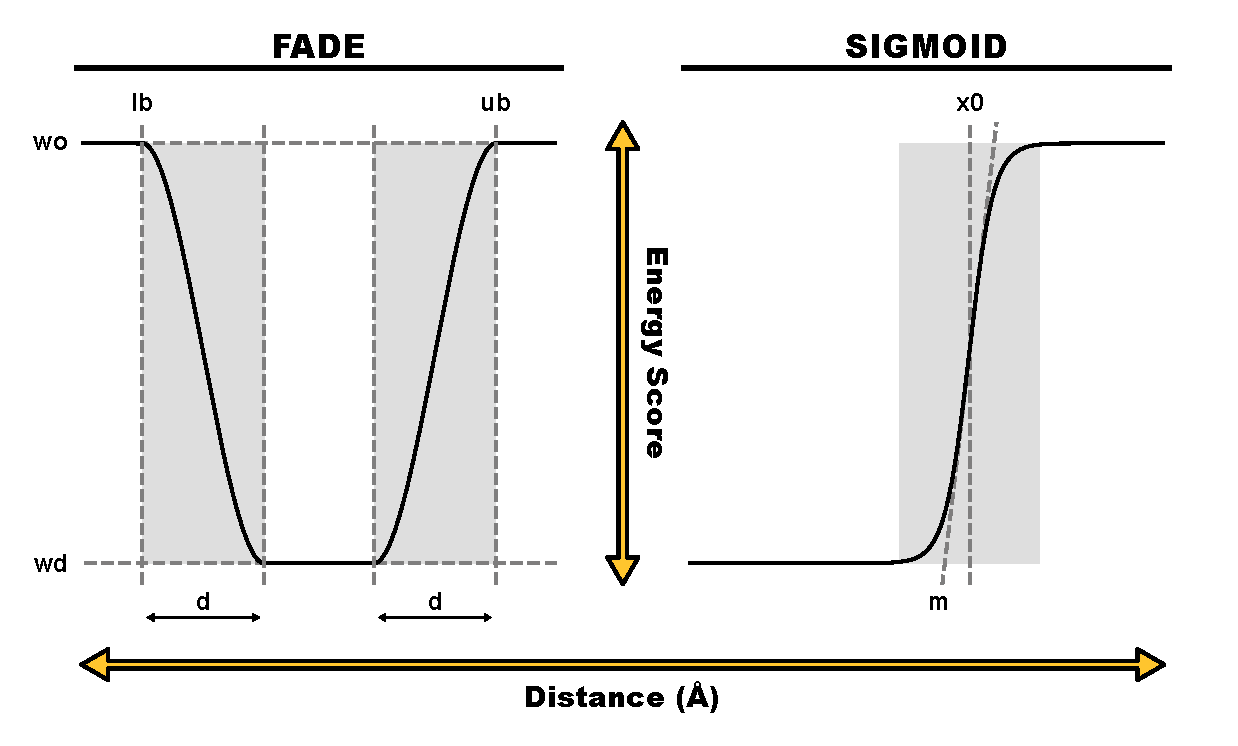
\includegraphics[width=\textwidth]{ample_predictors_efuncs.pdf}
    \caption{ROSETTA energy function comparison. Abbreviations corresponds to input parameters.}
    \label{fig:ample_predictors_efuncs}
\end{figure}

To explore the effects of the varying energy function definitions, we created six lists of contact restraints for each \textalpha-helical target and nine lists for each \textbeta-structure containing one. The top-ranking contact pairs per prediction were converted using the PCONSFOLD definition of the FADE function \cite{Michel2014-ci}, the GREMLIN definition of the SIGMOID function \cite{Ovchinnikov2015-nt}, and additionally the PCONSC2 BBCONTACTS definition of the FADE function for \textbeta-structure containing targets \textcolor{red}{(see Chapter XYZ)}.

The conversion was handled in \gls{ample} \textcolor{red}{(see Chapter XYZ)} and invoked with the keywords outlined in \cref{table:ample_predictors_kwargs}. The \texttt{-restraints\_factor} keyword defines the factor used to select contact pairs based on the target chain length, i.e. a factor of \texttt{1.5} would correspond to 3\textit{L}/2 contact pairs. The \texttt{-distance\_to\_neighbour} keyword defines the minimum distance in sequence space between contact pair participating residues, which were set to \texttt{5} residues for the FADE function \cite{Michel2014-ci} and \texttt{3} for the SIGMOID function \cite{Ovchinnikov2015-nt}. Additionally, all distance restraints were given an additional weight when introduced via the SIGMOID energy function to balance its energy term with all remaining terms in the ROSETTA scoring function (Sergey Ovchinnikov, personal communication). This was achieved by using the \texttt{-restraints\_weight} keyword and weights of \texttt{1.0} and \texttt{3.0} for the FADE and SIGMOID energy functions.

The addition of BBCONTACTS to existing sets of contacts was achieved with the FADE function in an identical manner as described in \textcolor{red}{Chapter XYZ}. In comparison, the SCALARWEIGHTED term in the GREMLIN implementation of the SIGMOID energy function \cite{Ovchinnikov2015-nt} was multiplied by the number of occurrences of each contact pair in the combined map.

\begin{table}[H]
    \centering
	\caption{Summary of \gls{ample} keyword arguments for FADE and SIGMOID ROSETTA energy functions.}
    \label{table:ample_predictors_kwargs}
    \begin{tabularx}{\textwidth}{ s b }
        \hline
        \textbf{Energy Function} & \textbf{\gls{ample} keywords} \\
        \hline
        \multirow{6}{1em}{FADE} & \texttt{-contact\_file <FILENAME>} \\
                                & \texttt{-contact\_format <FORMAT>} \\
                                & \texttt{-energy\_function FADE} \\
                                & \texttt{-restraints\_factor 1.0} \\
                                & \texttt{-distance\_to\_neighbour 5} \\
                                & \texttt{-restraints\_weight 1.0} \\
        \hline
        \multirow{6}{1em}{FADE (BBCONTACTS)} & \texttt{-contact\_file <FILENAME>} \\
                                & \texttt{-contact\_format <FORMAT>} \\
                                & \texttt{-energy\_function FADE} \\
                                & \texttt{-restraints\_factor 1.0} \\
                                & \texttt{-distance\_to\_neighbour 5} \\
                                & \texttt{-restraints\_weight 1.0} \\
        \hline
        \multirow{6}{1em}{SIGMOID} & \texttt{-contact\_file <FILENAME>} \\
                                & \texttt{-contact\_format <FORMAT>} \\
                                & \texttt{-energy\_function SIGMOID} \\
                                & \texttt{-restraints\_factor 1.5} \\
                                & \texttt{-distance\_to\_neighbour 3} \\
                                & \texttt{-restraints\_weight 3.0} \\
        \hline
        \multirow{6}{1em}{SIGMOID (BBCONTACTS)} & \texttt{-contact\_file <FILENAME>} \\
                                & \texttt{-contact\_format <FORMAT>} \\
                                & \texttt{-energy\_function SIGMOID\_bbcontacts} \\
                                & \texttt{-restraints\_factor 1.5} \\
                                & \texttt{-distance\_to\_neighbour 3} \\
                                & \texttt{-restraints\_weight 3.0} \\
        \hline
    \end{tabularx}
\end{table}

\subsection{\textit{Ab initio} structure prediction}
Six or nine individual lists of contact restraints generated for each target were used in separate ROSETTA \textit{ab initio} protein structure prediction runs. Additionally, protein structures were predicted without any contact restraints to acquire a control set of decoys. Homologous fragments were excluded during fragment library generation to imitate the folding process of a target with unknown fold. Fragment libraries were generated once per target and used throughout. In total, 1,000 \textit{ab initio} decoys were generated per run using ROSETTA’s default settings \cite{Rohl2004-ou} and one of the seven contact conditions described previously. In total, 162 sets of models were generated across 18 protein targets.

\subsection{\acrlong{mr}}
Besides considering model quality, one key interest of this study was the assessment of the model sets created in the previous step as \textit{ab initio} \gls{mr} search model templates. To reduce the enormous computational cost linked to trialling 162 sets of models, 108 sets were chosen from the following conditions: simple Rosetta, PCONSC2 prediction and FADE function, GREMLIN prediction and SIGMOID function, METAPSICOV prediction and FADE function, and where applicable, PCONSC2 BBCONTACTS, GREMLIN BBCONTACTS and METAPSICOV STAGE 1 BBCONTACTS predictions and FADE function. Overall, this resulted in four \gls{mr} runs for the six \textalpha-helical targets, seven runs for the six all-\textbeta, and seven runs for the six mixed \textalpha-\textbeta\ targets. The resulting 108 model sets were trialled in \gls{ample} v1.1.0. Structure solution success was assessed as described in \cref{sec:methods_mr_success}.

\section{Results}
\subsection{Direct comparison of three contact metapredictors}
In this study, a direct comparison between three metapredictors - GREMLIN, METAPSICOV and PCONSC2 - was carried out. Residue-residue contact pairs were predicted for 18 protein target sequences with a range of chain lengths and numbers of effective sequences in their Pfam sequence alignments.

METAPSICOV is the most precise contact predictor across the protein target dataset in this study (\cref{fig:ample_predictors_cutoff}). The difference between the three metapredictors is most evident in the highest-scoring contact pairs (\textit{L}/10). The median precision values for METAPSICOV and PCONSC2 contact predictions are above 50\% up to \textit{L} contact pairs. GREMLIN, in comparison, predicts contacts with a median precision score at least 20\% worse than that of METAPSICOV and 15\% worse than PCONSC2. However, at 3\textit{L}/2 contact pairs the median precision scores are much more similar across the three different metapredictors: METAPSICOV and PCONSC2 are near identical, and GREMLIN is at most 12\% worse compared to the other two. Inspecting the mean precision scores over a continuous range of selection cutoff values illustrates further the difference between METAPSICOV, PCONSC2 and GREMLIN (Fig \ref{fig:ample_predictors_covprc}). The former two similarly high precision scores compared to the average precision scores for GREMLIN, which are ~0.2 precision score units lower. Added to the difference in precision scores is the difference in sequence coverage (\cref{fig:ample_predictors_covprc}). Although producing the on-average worst contact predictions out of the three metapredictors used in this study, GREMLIN contact predictions have the highest sequence coverage. However, an analysis of singleton contact pairs, usually with high degrees of false positives, revealed a positive correlation ($\rho_{Pearson}=0.47$; $p<0.001$) between the fraction of singleton contact pairs and sequence coverage and hints to a weak negative correlation ($\rho_{Pearson}=-0.27$; $p<0.05$) between the fraction of singleton contact pairs and contact precision (\cref{fig:ample_predictors_singletons}).

\begin{figure}[H]
    \centering
    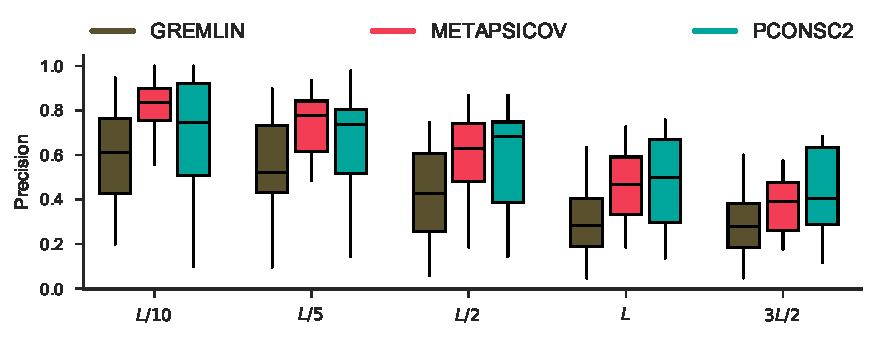
\includegraphics[width=\textwidth]{ample_predictors_cutoff.pdf}
    \caption{Precision spread for three metapredictors computed at five contact selection cutoff values relative to the target chain length (\textit{L}).}
    \label{fig:ample_predictors_cutoff}
\end{figure}

\begin{figure}[H]
    \centering
    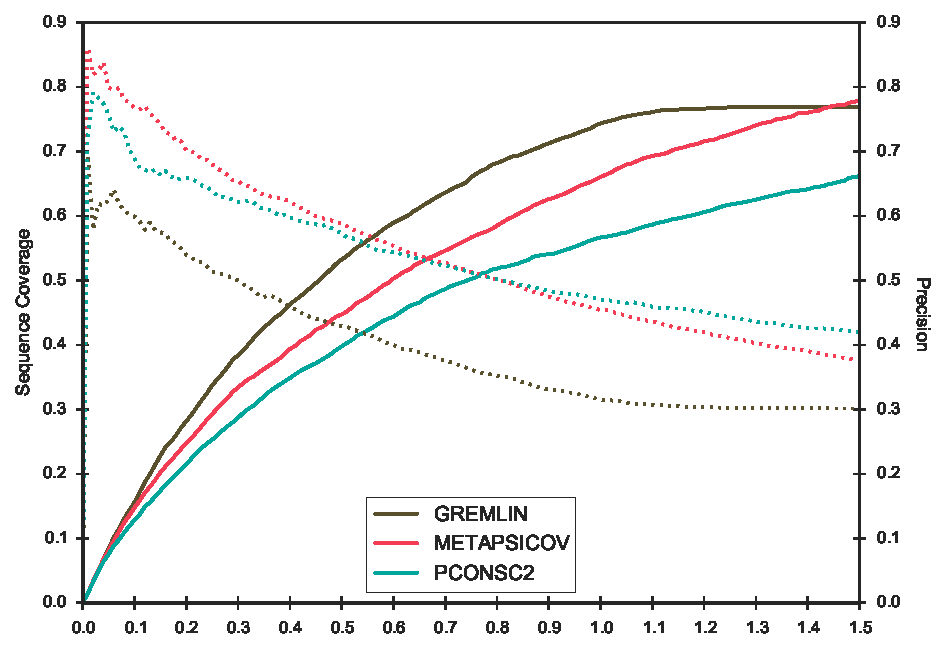
\includegraphics[width=\textwidth]{ample_predictors_covprc.pdf}
    \caption{Average sequence coverage (line) and contact prediction precision scores (dashed) across a continuous range of contact selection cutoffs ranging from $[0.0, 1.5]$ for all targets.}
    \label{fig:ample_predictors_covprc}
\end{figure}

\begin{figure}[H]
    \centering
    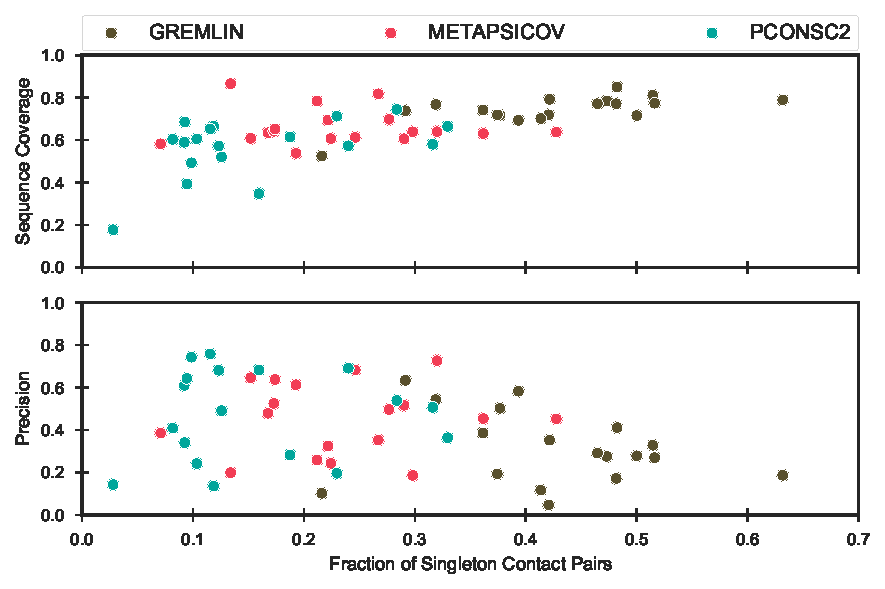
\includegraphics[width=\textwidth]{ample_predictors_singletons.pdf}
    \caption{Contact singleton analysis compared against the precision of \textit{L} contact pair lists for three metapredictors.}
    \label{fig:ample_predictors_singletons}
\end{figure}

Given that the overall precision of contact pairs predicted by the three metapredictors differs, it is important to understand where the difference originates. To investigate this, a comparison of the precision values at different cutoff levels on a per-target basis was performed. For the majority of targets the precision scores are very similar across the three metapredictors (\cref{fig:ample_predictors_prcpeaks}). However, the prediction precision of some targets differs significantly. For example, the METAPSICOV prediction for the human retinoic acid nuclear receptor HRAR (\gls{pdb}: 1fcy) contains high precision in its highest scoring (top-\textit{L}/10) contact pairs (\cref{fig:ample_predictors_prcpeaks}). In comparison, GREMLIN and PCONSC2 predictions for the same target contain less precise contact pairs ($\Delta Precision_{METAPSICOV-GREMLIN} L/10=-0.522$; $\Delta Precision_{METAPSICOV-PCONSC2} L/10=-0.435$). However, the addition of further contact pairs up to 3\textit{L}/2 results in near-identical precision across the three metapredictors for this target. A second example illustrating such a difference are the contact predictions for the human galectin-3 CRD sequence (\gls{pdb}: 4lbj). In contrast to the previous example, the data shows high precision scores for the METAPSICOV and PCONSC2 predictions for this target, yet low precision for the top GREMLIN contact pairs ($\Delta Precision_{METAPSICOV-GREMLIN} L/10=-0.231$; $\Delta Precision_{METAPSICOV-PCONSC2} L/10=+0.077$). 

\begin{figure}[H]
    \centering
    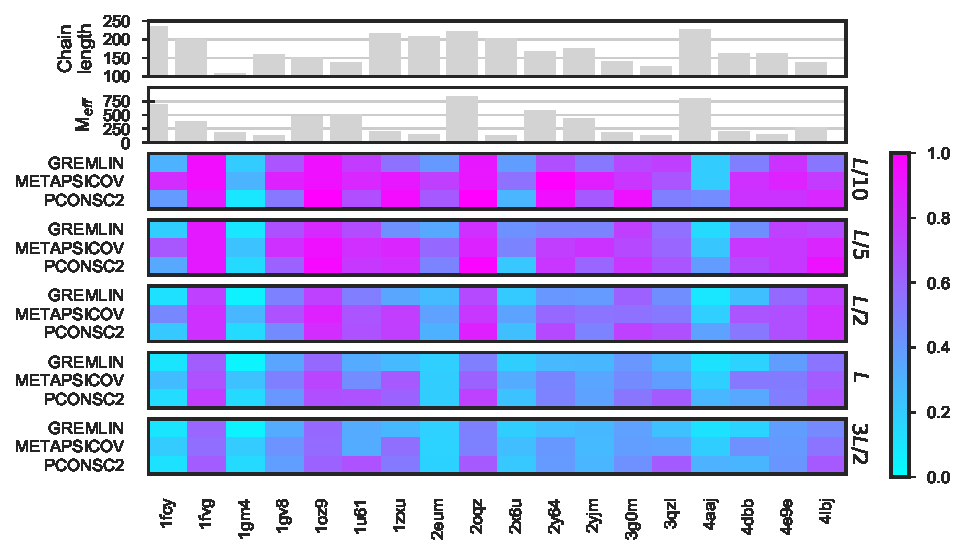
\includegraphics[width=\textwidth]{ample_predictors_prcpeaks.pdf}
    \caption{Contact prediction precision scores from three metapredictors for 18 targets at different contact pair selection thresholds. The Pfam alignment depth is given by means of number of effective sequences (\textit{Neff}). The color scale corresponds to the precision in $[0, 1]$.}
    \label{fig:ample_predictors_prcpeaks}
\end{figure}

The data presented in \cref{fig:ample_predictors_prcpeaks} also indicates that there is no direct link between chain length or Neff and the precision of the resulting contact predictions. The N-(5'-phosphoribosyl)anthranilate isomerase sequence (\gls{pdb}: 4aaj) with a chain length of 228 residues and 750 effective sequences in its Pfam alignment yielded a mean precision at \textit{L}/10 contact pairs of 0.283 (top-\textit{L}: 0.195) across the three metapredictors. This strongly contrasts with the sequence of sortase B (\gls{pdb}: 2oqz), which shows similar characteristics yet obtained  mean precision at \textit{L}/10 contact pairs of 0.938 (top-\textit{L}: 0.622).

Although the contact predictions differ in precision, an interesting question rests with the similarity of the predicted contact pairs amongst the sets. Thus, the similarity of contact predictions across the three metapredictors is an important metric to evaluate the most appropriate algorithm for \gls{ample} users. Using the Jaccard similarity index to evaluate the direct overlap of contact pairs across sets of predictions, the data suggests very little similarity between the contact predictions of the three metapredictors for each target (\cref{fig:ample_predictors_jaccardidx}). As with the differences in precision scores at higher cutoff thresholds, the Jaccard index is also lower - indicating less overlap - at higher cutoff thresholds. However, it is worth noting that the Jaccard index only considers identical matches and does not consider the neighbourhood of a contact pair. Thus, the index does not highlight similar regions with contact pairs in both maps.

\begin{figure}[H]
    \centering
    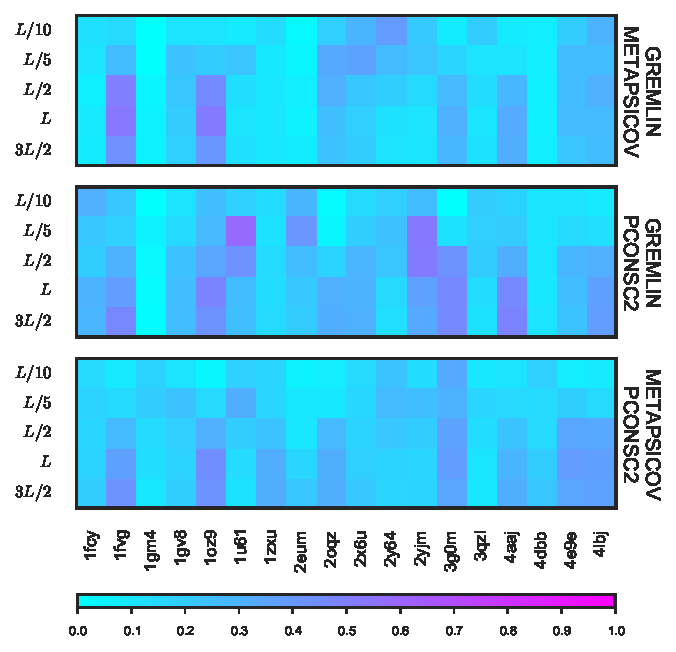
\includegraphics[width=\textwidth]{ample_predictors_jaccardidx.pdf}
    \caption{Jaccard similarity index illustrates a higher degree of overlap between metapredictor contact predictions with increasing numbers of contact pairs included in the calculation. The three panels show the different comparisons. The color scale corresponds to the Jaccard index in $[0, 1]$.}
    \label{fig:ample_predictors_jaccardidx}
\end{figure}

\subsection{Protein structure prediction with two ROSETTA energy functions}
The accuracy of the starting decoys is a major factor for an \gls{ample} run to succeed \cite{Simkovic2016-jx, Thomas2017-lq}. Thus, the quality of the decoys is of great essence to this study. Given the two different ROSETTA energy functions, FADE and SIGMOID, all contacts predicted were subjected to individual \textit{ab initio} structure prediction runs. Additionally, all contact predictions were enriched with BBCONTACTS for all \textbeta-containing targets in separate trials. A total of 234,000 individual decoys were generated in this study through all permutations of targets, contact predictions and ROSETTA energy function combinations.

Separating these individual decoys solely by the ROSETTA energy function (excluding unrestrained ROSETTA decoys) shows that the FADE energy function results in marginally more accurate decoys (median TM-score FADE: 0.3541; median TM-score SIGMOID: 0.2969). To further investigate which energy function is more suitable for the target dataset used in this study, the decoy sets were grouped by two additional characteristics: the fold of the target, and the source of distance restraints used. The results strongly suggest that the FADE energy function results in more accurate decoy sets (\cref{fig:ample_predictor_tmmedian}), outperforming the SIGMOID energy function by median TM-score in two-thirds of all decoys sets (FADE: 58; SIGMOID: 32). A split of the decoy sets into separate categories by fold and the addition of BBCONTACTS reveals that the SIGMOID energy function only yields similar results for all-\textbeta\ targets in combination with BBCONTACTS-supported distance restraints. Although the total count of decoy sets with higher accuracies between the two energy functions in this category are similar, the actual differences in TM-scores further supports the strength of the FADE energy function compared to the SIGMOID.

\begin{figure}[H]
    \centering
    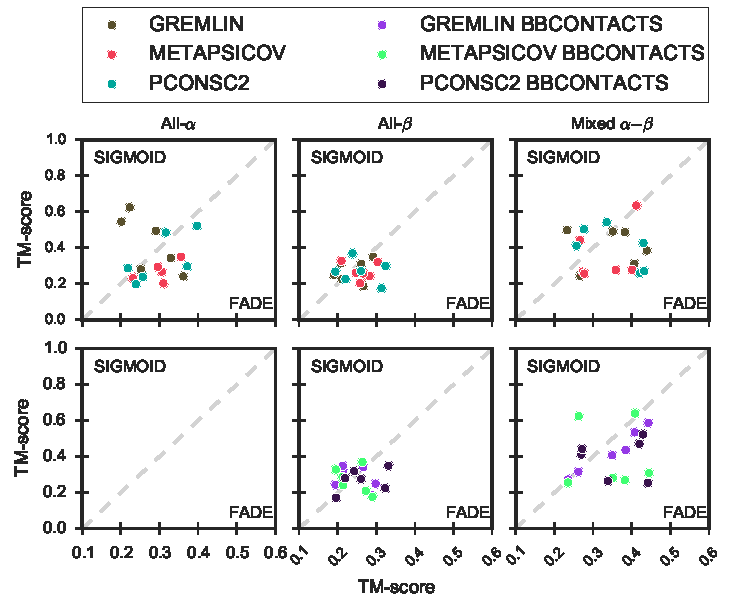
\includegraphics[width=\textwidth]{ample_predictors_tmmedian.pdf}
    \caption{Median TM-score comparison of FADE and SIGMOID ROSETTA energy functions differentiated by fold and the addition of BBCONTACTS restraints.}
    \label{fig:ample_predictor_tmmedian}
\end{figure}

Besides the structure prediction accuracy of each set of decoys, the single, most accurate decoy is also of great interest. If one energy function consistently predicts single decoys more accurately, it might be appropriate to reconsider the structure identification routine (i.e. clustering) in \gls{ample} for search model preparation. However, a similar difference to that of the decoy quality of entire sets is observed for the top-1 decoy in each set (\cref{fig:ample_predictor_tmtop}). The FADE energy function outperforms the SIGMOID function for the majority of target-contact prediction permutations (FADE: 51; SIGMOID: 39). However, the GREMLIN distance restraints in combination with the SIGMOID energy function produce better top-1 decoys than GREMLIN restraints with the FADE energy function. This suggests that GREMLIN restraints and the SIGMOID energy function were tailored to complement each other with the ultimate goal of predicting single decoys to high accuracy over entire sets of decoys. Additionally, the spread of decoy quality differences between the two energy functions widens when only looking at the best decoy in each predicted set ($\Delta Median TM-score_{ALL}: min=0.002, max=0.429$; $\Delta Median TM-score_{TOP}: min=0.002, max=0.456$). 

\begin{figure}[H]
    \centering
    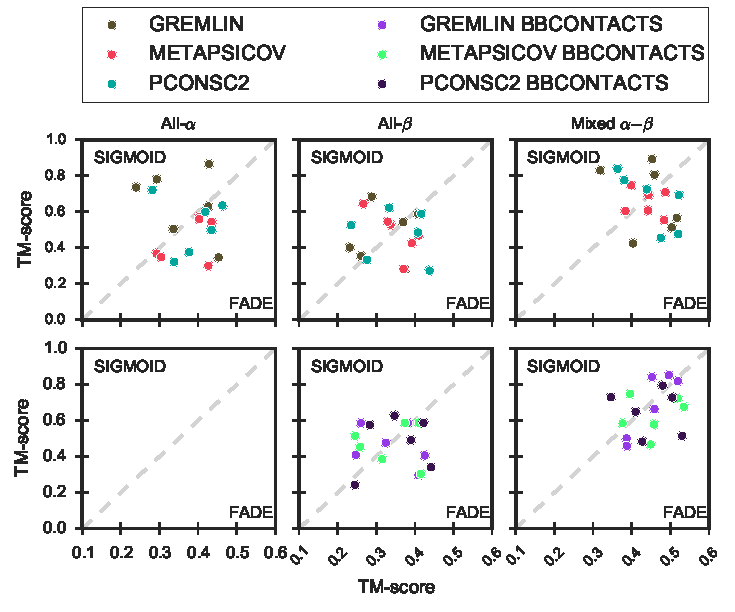
\includegraphics[width=\textwidth]{ample_predictors_tmtop.pdf}
    \caption{Top TM-score comparison of FADE and SIGMOID ROSETTA energy functions differentiated by fold and the addition of BBCONTACTS restraints.}
    \label{fig:ample_predictor_tmtop}
\end{figure}

A \acrfull{kde} of TM-scores using each predicted decoy was generated with the TM-scores of individual decoys separated only by fold class and ROSETTA energy function (\cref{fig:ample_predictor_tmdensity}). This density estimate further supports the results presented above: the FADE energy function generates more accurate decoys. However, a very important detail is highlighted by the estimates. Distinct regions with high density are visible in the estimates of the TM-scores of individual decoys for all-\textalpha\ and mixed \textalpha-\textbeta\ targets (\cref{fig:ample_predictor_tmdensity}). The bimodal distribution of decoy TM-scores from both energy functions strongly suggests that predicted structures are either native-like or not (based on the TM-score threshold of $\leq0.5$). However, the number of correctly predicted decoys versus incorrectly predicted decoys is in favour of the latter. The decoy sets of all-\textbeta\ targets do not show such distinct regions of high density for decoys with TM-scores $<0.5$ units in any of its density estimates (\cref{fig:ample_predictor_tmdensity}). The generally poor decoy quality of decoys predicted without any distance restraint information (ROSETTA) highlights the benefit of contact predictions to \textit{ab initio} protein structure prediction.

\begin{figure}[H]
    \centering
    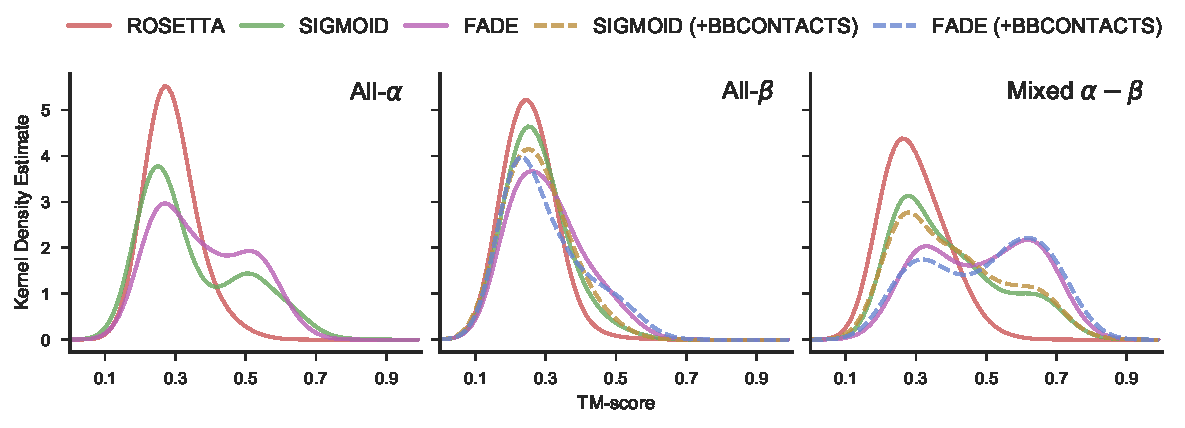
\includegraphics[width=\textwidth]{ample_predictors_tmdensity.pdf}
    \caption{TM-score density estimate of all decoys in each respective fold class separating by ROSETTA energy function (SIGMOID or FADE) and no contact information used (ROSETTA). Dashed lines indicate decoys which were predicted with the addition of BBCONTACTS.}
    \label{fig:ample_predictor_tmdensity}
\end{figure}

A further important aspect of this study is to explore the benefits of adding BBCONTACTS restraints to the structure prediction of \textbeta-containing targets. Although previous results \textcolor{red}{(see Chapter XYZ)} in combination with those presented above outline overall improvements in decoy quality, it is essential to understand which targets benefit from this treatment. Figure \ref{fig:ample_predictor_bbdir} highlights the effects of adding BBCONTACTS restraints to the structure prediction strategies employed here. In summary, the addition of BBCONTACTS restraints hardly affects the decoy quality of most targets under the various contact prediction and energy function combinations. Nevertheless, three target, contact prediction and energy function combinations yielded TM-score improvements of at least 0.1 TM-score units compared to the same condition without the addition of BBCONTACTS restraints. In contrast, the addition of BBCONTACTS restraints did not lower the median TM-score by more than 0.1 units for any target (\cref{fig:ample_predictor_bbdif}).

\begin{figure}[H]
    \centering
    \begin{subfigure}[b]{\textwidth}
        \centering
        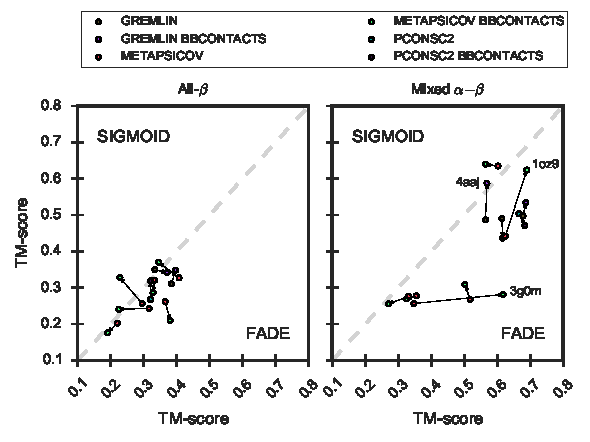
\includegraphics[width=0.9\textwidth]{ample_predictors_bbdir.pdf}
        \caption{}
        \label{fig:ample_predictor_bbdir}
    \end{subfigure}
    
    \begin{subfigure}[b]{\textwidth}
        \centering
        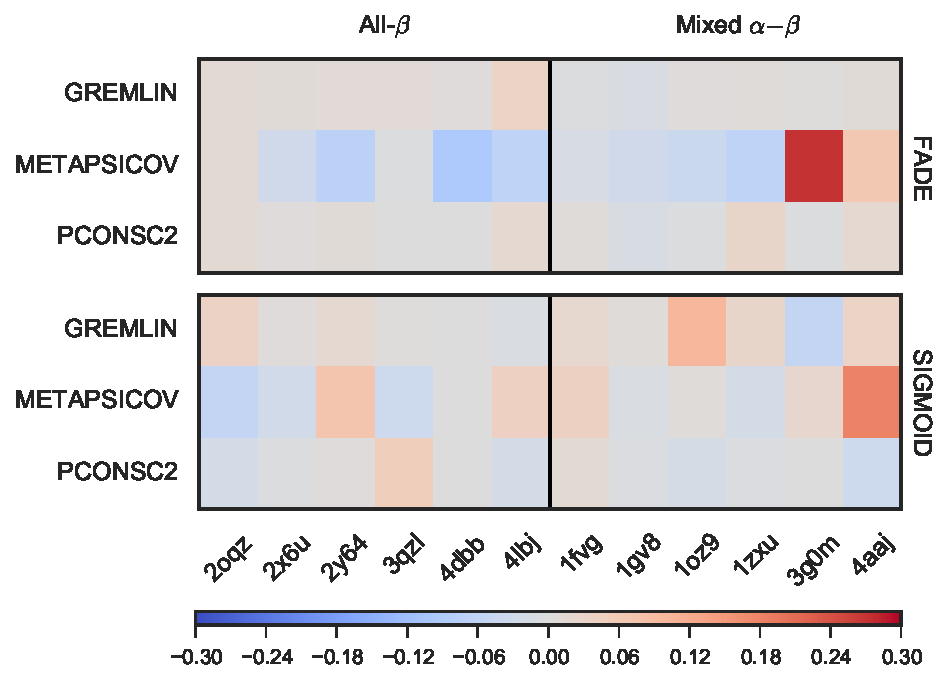
\includegraphics[width=0.9\textwidth]{ample_predictors_bbdif.pdf}
        \caption{}
        \label{fig:ample_predictor_bbdif}
    \end{subfigure}

    \caption{Median TM-score comparison of FADE and SIGMOID ROSETTA energy functions differentiated by fold (excl. all-\textalpha). (a) Arrows indicate the effect on decoy quality through the addition of BBCONTACTS restraints. Targets with a distance $<0.03$ TM-score units between normal and BBCONTACTS-added conditions were excluded from the scatter plots. (b) Effect on decoy quality through the addition of BBCONTACTS restraints highlighted by heatmap difference. The color scale corresponds to the difference in median TM-score between normal and BBCONTACTS-added contact maps.}
\end{figure}

Two further aspects in understanding the differences in effects of the FADE and SIGMOID ROSETTA energy functions on decoy quality are the target chain length and restraints precision. The former appears to affect the final decoy quality of all 1,000 decoys insignificantly (\cref{fig:ample_predictor_tmsummary}). However, the restraint precision results in some differences between the two ROSETTA energy functions (\cref{fig:ample_predictor_tmsummary}). The FADE energy function (L restraints) generally appears to be less sensitive to restraint lists with higher false positive contact pairs.  In contrast, the SIGMOID function  (3\textit{L}/2 restraints) produces less accurate decoys than the FADE function with more accurate restraints. Most strikingly, the FADE energy function generated decoys with a median TM-score of 0.678 for the N-(5'-phosphoribosyl)anthranilate isomerase domain (\gls{pdb}: 4aaj) compared to the SIGMOID function with a median TM-score of 0.498. Nevertheless, both energy functions appear to broadly follow a positive linear trend, i.e. better restraint precision results in more accurate decoys.

\begin{figure}[H]
    \centering
    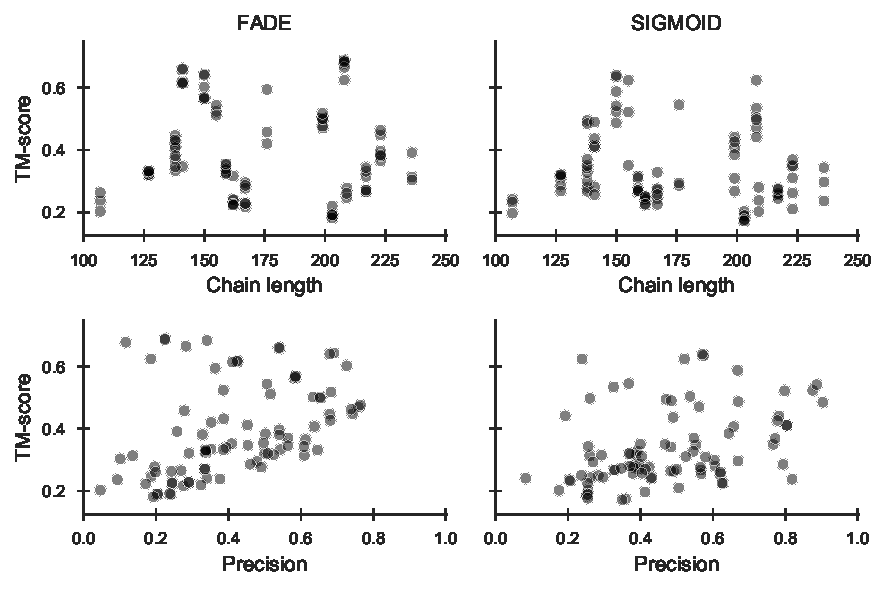
\includegraphics[width=\textwidth]{ample_predictors_tmsummary.pdf}
    \caption{Effects of target chain length and restraint precision on the median TM-score for FADE and SIGMOID ROSETTA energy functions. Each scatter point represents a 1,000-decoy set.}
    \label{fig:ample_predictor_tmsummary}
\end{figure}

\subsection{Impact of metapredictors and energy functions on unconventional \acrlong{mr}}
The results obtained from the decoy quality comparison outlined above highlighted differences between the FADE and SIGMOID ROSETTA energy functions. This difference is more pronounced for some targets and less so for others. Thus, the next step in this study was to analyse the consequences  of these differences for unconventional \gls{mr} using the automated pipeline \gls{ample}.

Overall, the decoys restrained with GREMLIN distance restraints via the SIGMOID energy function throughout the structure prediction process yielded six out of 18 possible structure solutions (\cref{fig:ample_predictor_ample}). This result was the highest of all trialled conditions and only resulted in one more structure solution compared to unrestrained ROSETTA decoys. All remaining conditions resulted in fewer structure solutions than those from ROSETTA decoys. Furthermore, the conditions METAPSICOV (FADE function), METAPSICOV BBCONTACTS (FADE function) and PCONSC2 BBCONTACTS (FADE function) yielded no more than half of the structure solutions achieved by GREMLIN (SIGMOID function). The remaining two conditions - PCONSC2 (FADE function) and GREMLIN BBCONTACTS (FADE function) - resulted in four out of 18 structure solutions. The addition of BBCONTACTS did not improve decoy quality enough to increase the chances of structure solution success; however, the structure of the bovine peptide methionine sulfoxide reductase (\gls{pdb}: 1fvg) was only solved with the GREMLIN BBCONTACTS (FADE function) decoys further supporting the small but important value of BBCONTACTS restraint addition to separately determined contact predictions \textcolor{red}{(see Chapter XYZ)}.

\begin{figure}[H]
    \centering
    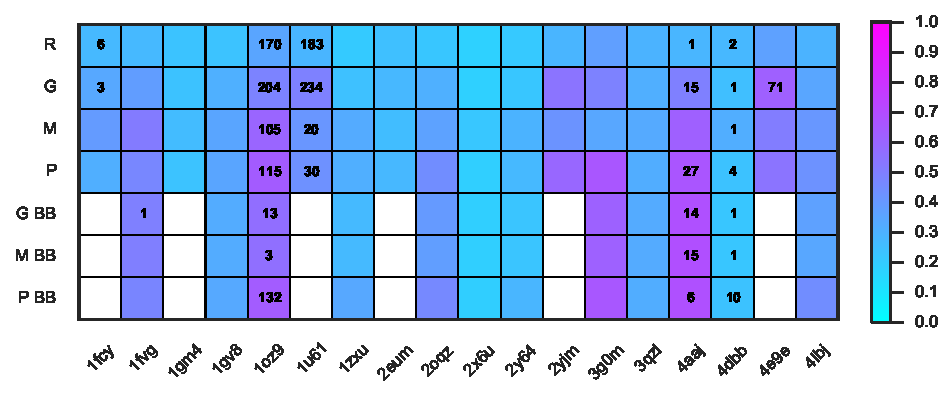
\includegraphics[width=\textwidth]{ample_predictors_ample.pdf}
    \caption{Structure solution count for \gls{ample} search models generated from decoys with varying contact prediction and ROSETTA energy function conditions: unrestrained ROSETTA (R); GREMLIN (G; SIGMOID function); METAPSICOV (M; FADE function); PCONSC2  (P; FADE function); GREMLIN BBCONTACTS (G BB; FADE function); METAPSICOV BBCONTACTS (M BB; FADE function); PCONSC2 BBCONTACTS (P BB; FADE function). The color scale of each square indicates the median TM-score of all 1,000 starting decoys.}
    \label{fig:ample_predictor_ample}
\end{figure}

The number of structure solutions obtained from the decoy sets subjected to the \gls{ample} pipeline are somewhat surprising given that ROSETTA decoys result in the second-most structure solutions. These results suggest that the current implementation cannot exploit the true value of more accurate decoy sets. This hypothesis is further supported when considering the decoy set quality and the number of structure solutions (\cref{fig:ample_predictor_ample}). For example, PCONSC2 (FADE function) decoys predicted for the hypothetical protein AQ\_1354 (\gls{pdb}: 1oz9) yield high accuracy, and thus would generally be considered highly desirable starting structures for the \gls{ample} protocol; nevertheless, the \gls{ample} protocol was unable to exploit such highly accurate decoys for successful structure solutions of other targets, e.g. cysteine desulferation protein SufE (\gls{pdb}: 3g0m; $median TM-score PCONSC2 BBCONTACTS (FADE function)=0.661$). In comparison, the median TM-scores for all successful ROSETTA decoy sets do not exceed 0.355 TM-score units.

Naturally, one would expect the best decoys to result in the most accurate ensemble search models, which in turn yield the highest number of structure solutions per target. However, here we demonstrate that the most accurate decoys do not guarantee structure solution, and in contrast some poorly predicted decoy sets achieve structure solution. Thus, it is essential to investigate the stage in \gls{ample}’s cluster-and-truncate approach at which the higher decoy quality results in less suitable ensemble search models for \gls{mr}.

The data generated as part of this study reveals a positive correlation ($\rho_{Spearman}=0.78$; $p<0.001$) between the decoy quality and the number of resulting \gls{ample} ensemble search models (\cref{fig:ample_predictor_ensdep}). The plotted data alongside a fitted LOWESS function further illustrate that small differences in decoy quality in the lower TM-score regions increases the total number of generated ensemble search models dramatically. However, once the threshold of 0.5 TM-score units \cite{Xu2010-sw} is surpassed the number of generated ensemble search models plateaus at around ~350-400 ensemble search models, approaching the maximum number of search models generatable by \gls{ample}. Furthermore, the data suggests that sets containing fewer than 100 ensemble search models do not lead to structure solution, although this result needs to be considered with care given the difficulty of predicting which search model will lead to structure solution.

\begin{figure}[H]
    \centering
    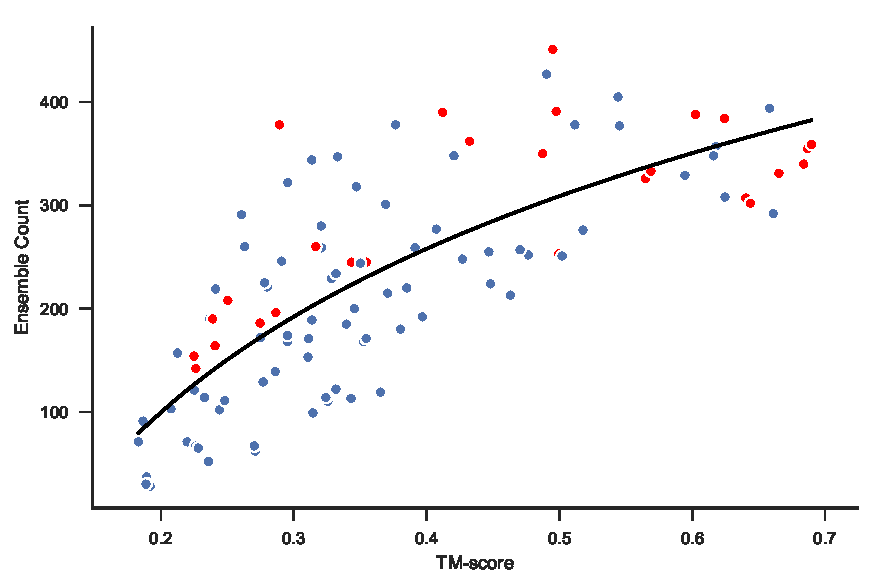
\includegraphics[width=\textwidth]{ample_predictors_ensdep.pdf}
    \caption{Comparison of median TM-score comparison (per 1,000 decoys) against the resulting \gls{ample} ensemble search model count. LOWESS function fitted to data to illustrate relationship. Red dots indicate successful ensemble sets.}
    \label{fig:ample_predictor_ensdep}
\end{figure}

Besides looking at the relationship between entire decoy sets and the resulting structure solutions on a per-target or per-condition basis, it is important to also consider individual ensemble search models, their origins and their properties in relation to \gls{mr} metrics. Previous findings highlighted the relationship between the number of decoys in the first cluster and the quality of the decoys it contains \textcolor{red}{(see Chapter XYZ)}. Here, we further support these findings given the positive relationship between the median TM-scores and the corresponding size of the largest SPICKER cluster (\cref{fig:ample_predictor_clusizetm}). An analysis of the cluster sizes demonstrates the downstream benefits of increased decoy quality through contact restraints in the folding process (\cref{fig:ample_predictor_clusize}). The sizes of the first three clusters generated from most contact-restraint decoy sets greatly surpass their equivalent cluster sizes for unrestrained ROSETTA decoys. Given that cluster sizes correlate with decoy quality, the findings in this study also support that the mean C\textalpha\ \gls{rmsd} - as calculated by THESEUS for cluster truncation - is directly related to better decoy quality via the larger number of decoys in each cluster (\cref{fig:ample_predictor_clurmsd}). The same mean C\textalpha\ \gls{rmsd} is also related to the number of ensemble search models generated after subclustering (\cref{fig:ample_predictor_rmsdsm}), which hints towards a direct relationship between increased quality of 1,000 decoys per set and the total number of ensemble search models generated. Interestingly, GREMLIN decoys show similar C\textalpha\ \gls{rmsd} per cluster compared to unrestrained ROSETTA decoys (\cref{fig:ample_predictor_carmsd}), unlike all other contact restraint guided structure predictions. However, it is worth noting that almost no distinction can be made amongst the remaining contact restraint treatments albeit some differences in cluster size distributions exist (\cref{fig:ample_predictor_clusize}).

\begin{figure}[H]
    \centering
    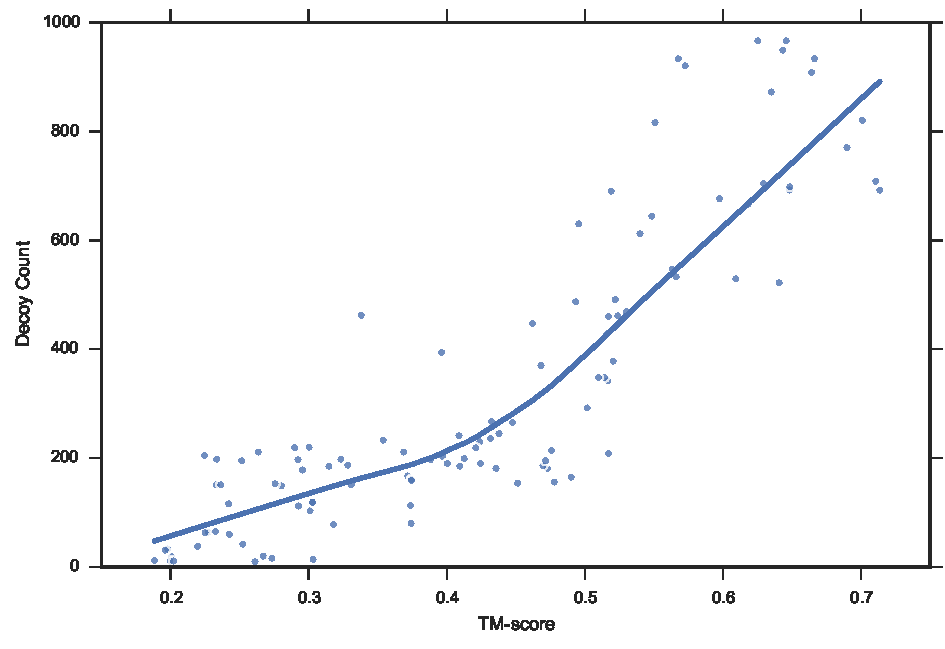
\includegraphics[width=\textwidth]{ample_predictors_clusizetm.pdf}
    \caption{Relationship between cluster median TM-score and the number of cluster decoys. Blue line represents LOWESS relationship fitted to data.}
    \label{fig:ample_predictor_clusizetm}
\end{figure}

\begin{figure}[H]
    \centering
    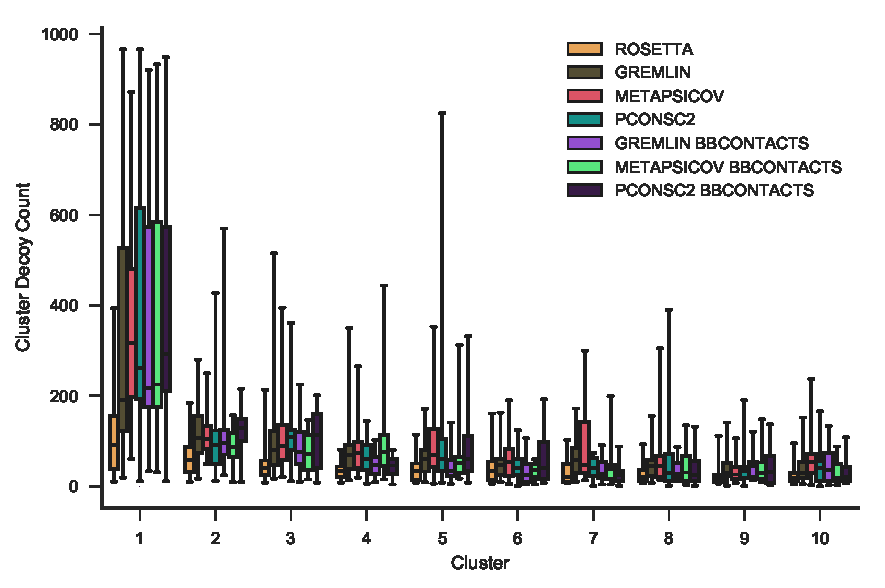
\includegraphics[width=\textwidth]{ample_predictors_clusize.pdf}
    \caption{SPICKER cluster sizes of each target grouped the restraint condition used during the structure prediction protocol. Whiskers span the range from the minimum to maximum counts.}
    \label{fig:ample_predictor_clusize}
\end{figure}

\begin{figure}[H]
    \centering
    \begin{subfigure}[b]{\textwidth}
        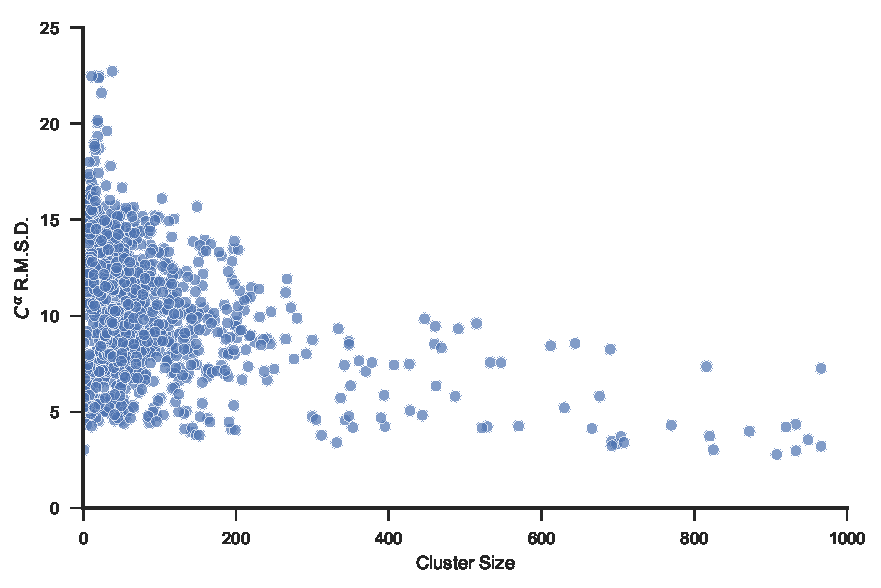
\includegraphics[width=\textwidth]{ample_predictors_clurmsd.pdf}
        \caption{}
        \label{fig:ample_predictor_clurmsd}
    \end{subfigure}
    \begin{subfigure}[b]{\textwidth}
        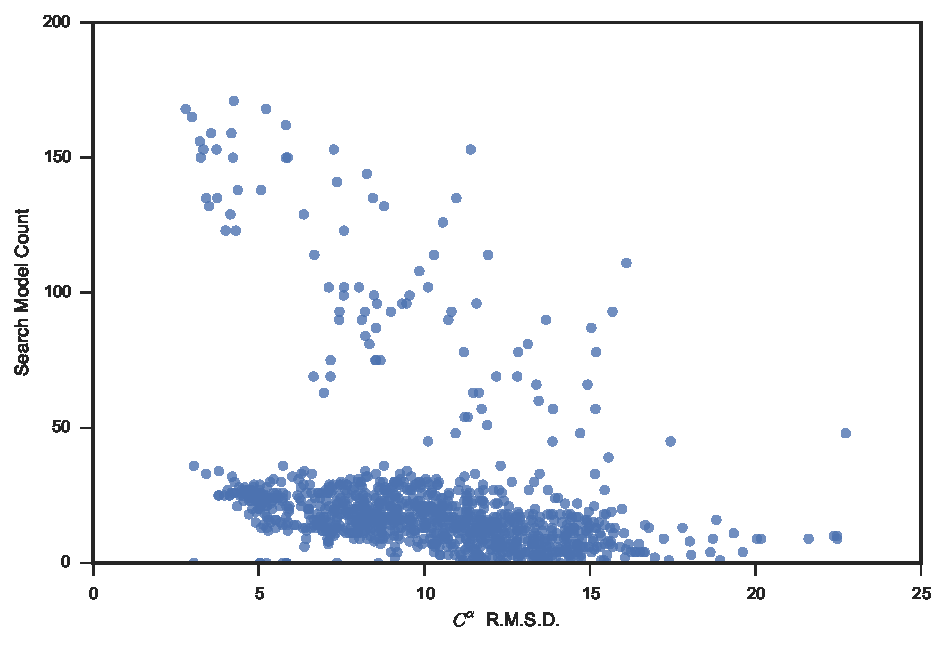
\includegraphics[width=\textwidth]{ample_predictors_rmsdsm.pdf}
        \caption{}
        \label{fig:ample_predictor_rmsdsm}
    \end{subfigure}

    \caption{(a) Number of decoys per SPICKER cluster plotted against the mean C\textalpha-atom \gls{rmsd} for all decoys in each cluster. (b) Mean C\textalpha-atom \gls{rmsd} for decoys per cluster plotted against the number of search models derived from the cluster.}
\end{figure}

\begin{figure}[H]
    \centering
    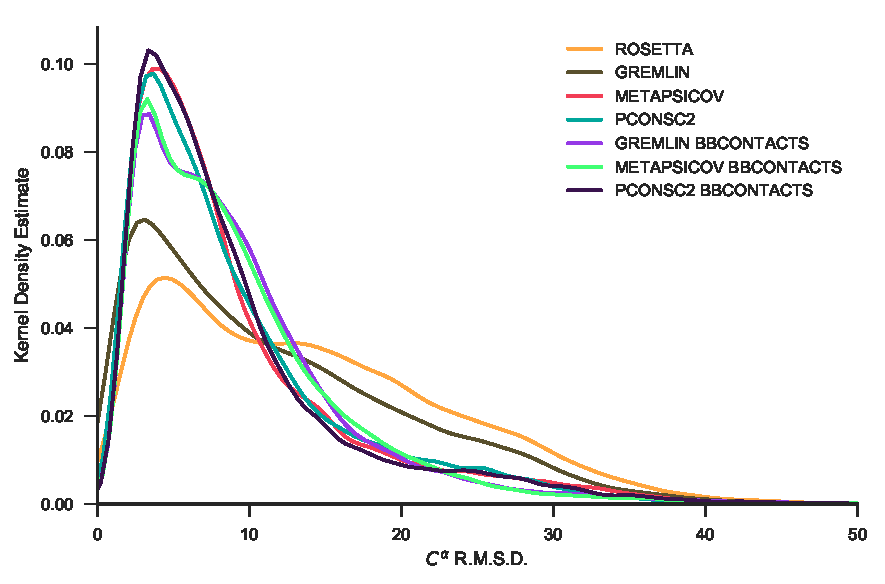
\includegraphics[width=\textwidth]{ample_predictors_carmsd.pdf}
    \caption{Kernel density estimate of C\textalpha\ interatomic \gls{rmsd} for SPICKER clusters.}
    \label{fig:ample_predictor_carmsd}
\end{figure}

The structure solution through pipelines like \gls{ample} and other unconventional \gls{mr} software \cite{Rodriguez2009-tk, Sammito2013-tt} can result from the placement of generated (ensemble) search models either in- or out-of-sequence register. The RIO metric \cite{Thomas2015-ag} can reliably assess the register placement, and thus was used to analyse the \gls{mr} placements of all search models of the seven targets with structure solutions from one or more decoy sets. The RIO scores for the hypothetical protein AQ\_1354 (\gls{pdb}: 1oz9) strongly support the high quality decoys used as input across all seven contact conditions (\cref{fig:ample_predictor_riotar}). Most search models are placed in-register and hardly any search models with out-of-register RIO scores failed either. In contrast, the search models of N-(5’-phosphoribosyl)anthranilate isomerase (\gls{pdb}: 4aaj) - derived from high quality decoys in most conditions - shows a low percentage of \gls{ample} search models with RIO scores leading to structure solution (\cref{fig:ample_predictor_riotar}). Furthermore, the RIO scores normalized by the target chain length indicate that search models, independent of \gls{mr} structure solution, were relatively small only exceeding 20\% of the total target sequence in a few cases. 

\begin{figure}[H]
    \centering
    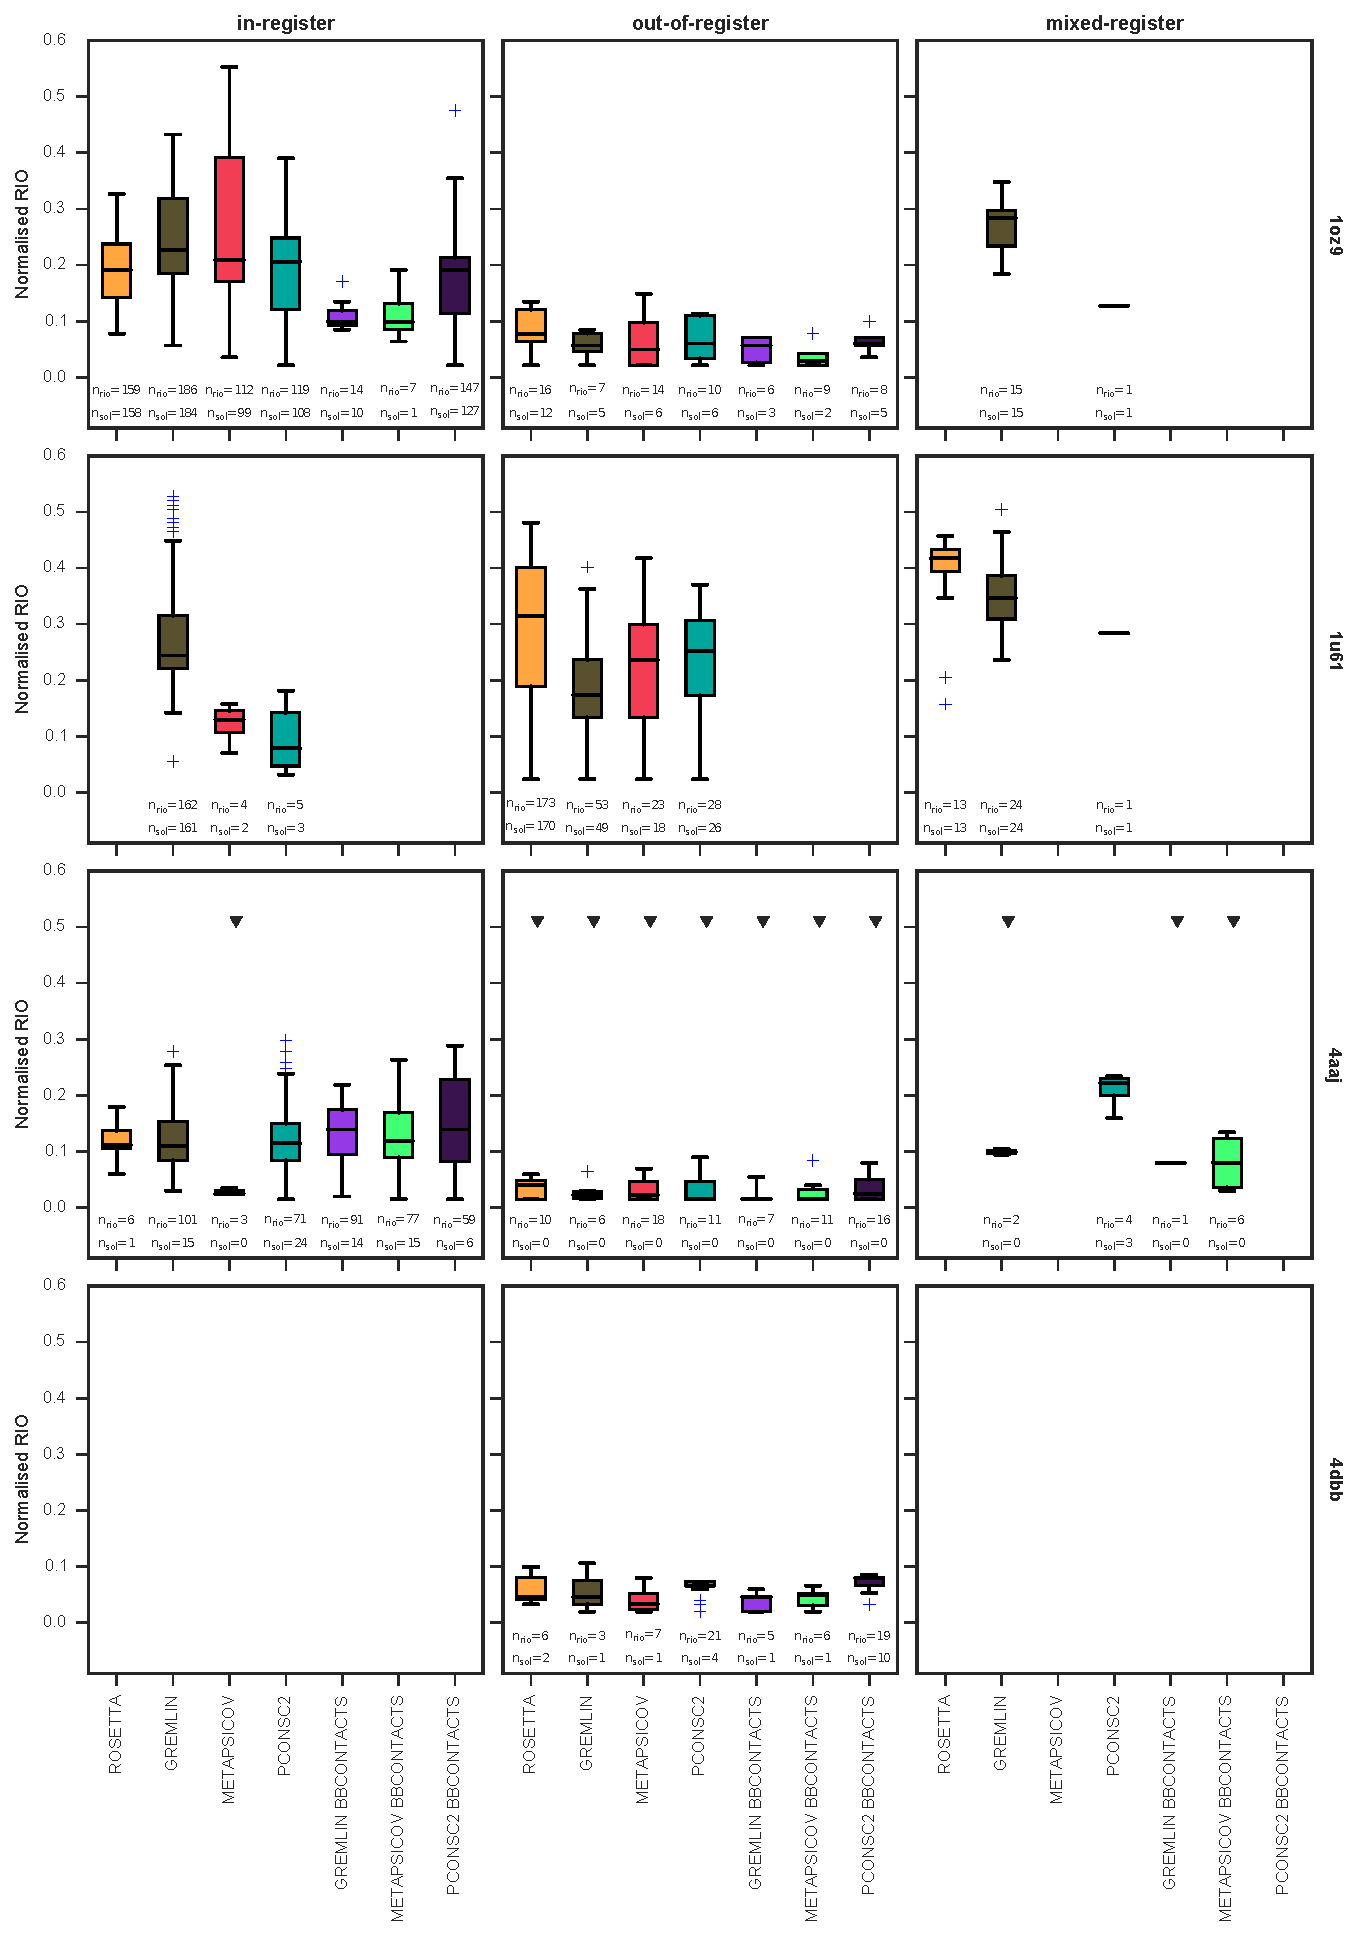
\includegraphics[width=\textwidth]{ample_predictors_riotar.pdf}
    \caption{Normalised RIO score analysis of four successful targets in the \gls{mr} dataset. Black triangles indicate \gls{ample} search model sets without a structure solution.}
    \label{fig:ample_predictor_riotar}
\end{figure}

One interesting target in this set with respect to the sequence register of the \gls{ample} search models leading to structure solution is putative ribonuclease III (\gls{pdb}: 1u61). Although decoys from all contact conditions readily solved this target with at least 20 or more \gls{ample} search models, one interesting aspect arises from the RIO register analysis. Only GREMLIN decoys are primarily placed in-register (\cref{fig:ample_predictor_riotar}). \gls{ample} search models derived from the other three contact conditions, and in particular those from ROSETTA decoys, are primarily placed out-of-register with sequence coverage values of roughly 25\%. In fact, a close analysis of the diversity of \gls{ample} search models highlights the accuracy of GREMLIN search models which represent a closely-matched substructure of the target protein (\cref{fig:ample_predictors_1u61_c2_t70_r1_reliable}).  

\begin{figure}[H]
    \centering
    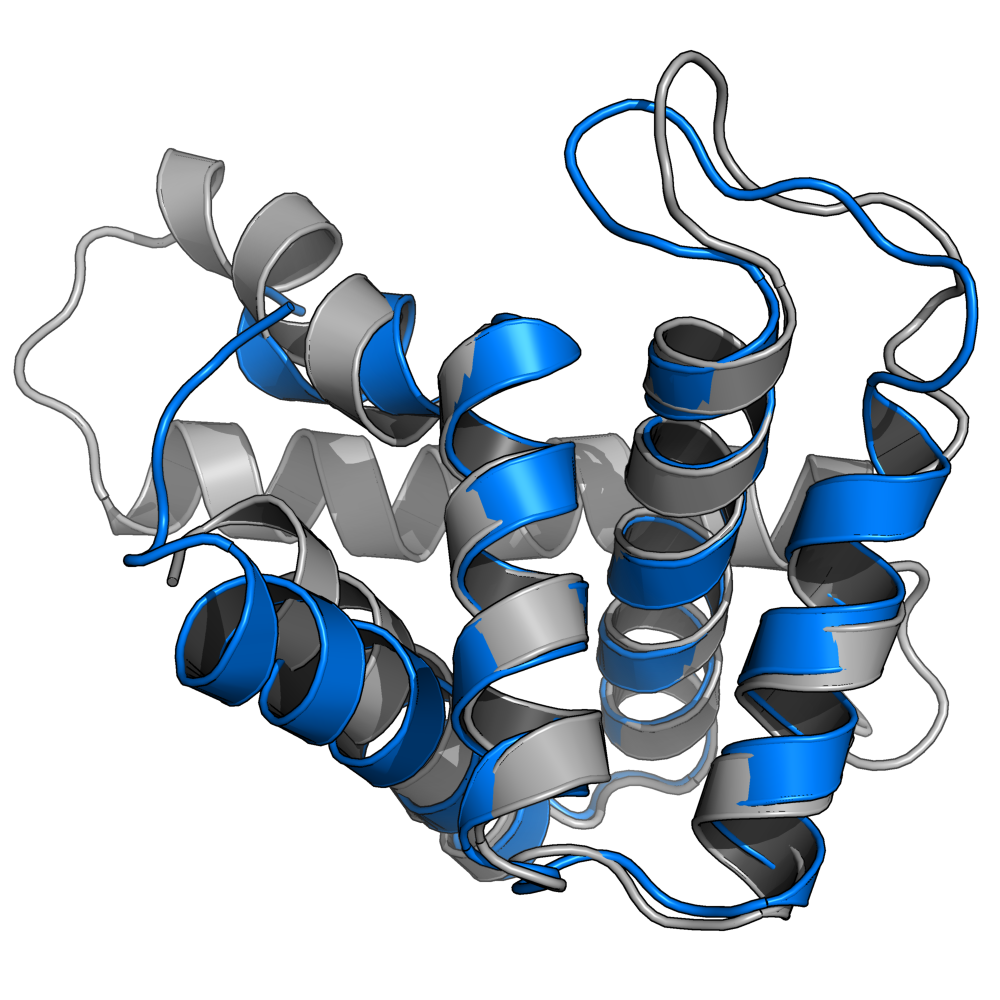
\includegraphics[width=\textwidth]{ample_predictors_1u61_c2_t70_r1_reliable.png}
    \caption{Successful search model (blue cartoon) post-PHASER placement superposed with the native structure (gray cartoon) for putative ribonuclease III (\gls{pdb}: 1u61).}
    \label{fig:ample_predictors_1u61_c2_t70_r1_reliable}
\end{figure}

Compared to all other targets with structure solutions in at least one condition, the PTB domain of Mint1 (\gls{pdb}: 4dbb) produced interesting yet somewhat surprising results. None of the search models, independent of their decoy source, achieved correct placement with any residue being in register. All structure solutions were obtained from out-of-register search model placements (\cref{fig:ample_predictor_riotar}). A visual inspection of all successful search models revealed that structure solutions were exclusively obtained with idealised fragments. ROSETTA, GREMLIN and METAPSICOV decoys resulted in one or more single-helix ensemble search models that led to structure solution (\cref{fig:ample_predictors_4dbb_esm_egs}). More interestingly though, PCONSC2, GREMLIN BBCONTACTS, METAPSICOV BBCONTACTS and PCONSC2 BBCONTACTS decoys yielded one or more two-strand \textbeta-sheets which, after successful \gls{mr}, yielded fully built structures (\cref{fig:ample_predictors_4dbb_esm_egs}).

\begin{figure}[H]
    \centering
    \includegraphics[width=\textwidth]{ample_predictors_4dbb_esm_egs.png}
    \caption{Successful search models post-PHASER placement (blue) superposed to the reference crystal structure (grey) for PTB domain of Mint1 (\gls{pdb}: 4dbb).}
    \label{fig:ample_predictors_4dbb_esm_egs}
\end{figure}

Lastly, three targets were solved with one or two decoy sets alone. The structures of the retinoic acid nuclear receptor HRAR (\gls{pdb}: 1fcy) and the peptide methionine sulfoxide reductase (\gls{pdb}: 1fvg) were only solved with a handful of \gls{ample} search models. Often singleton solutions like these are achieved through \gls{ample}’s cluster-and-truncate procedure producing a single, idealised helix as search model. Here, we confirm such findings for target 1fcy, whereby single out-of-register helices derived from ROSETTA and GREMLIN decoys achieved structure solutions. However, the singleton search model derived from the GREMLIN BBCONTACTS decoys for the peptide methionine sulfoxide reductase (\gls{pdb}: 1fvg) was placed in-register. A closer inspection of this \gls{ample} ensemble search model highlights a great success of the approach of adding BBCONTACTS distance restraints to separately predicted contact maps. In this instance, the successful \gls{ample} ensemble search model has 77\% of its 49 residues placed in-register. More importantly, the search model is made up of two \textbeta-strands packing against each other, which was supported by BBCONTACTS predictions (\cref{fig:ample_predictors_1fvg_gbb_phaser_c1_t25_r3_polyAla}). The last case, glycosylase domain of MBD4 (\gls{pdb}: 4e9e), solved solely with GREMLIN decoys yielding 71 structure solutions. All successful \gls{ample} search models derived from the GREMLIN decoys were placed in-register.

\begin{figure}[H]
    \centering
    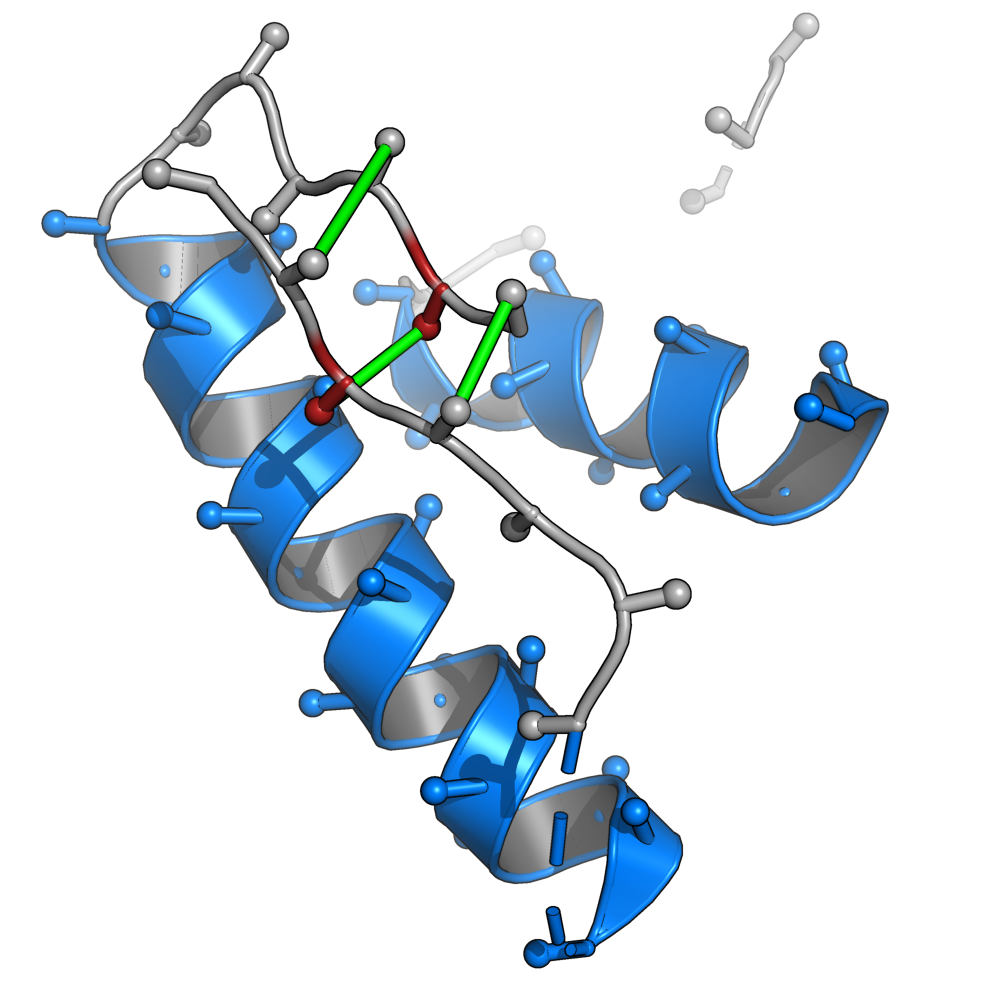
\includegraphics[width=\textwidth]{ample_predictors_1fvg_gbb_phaser_c1_t25_r3_polyAla.png}
    \caption{Successful search model post-PHASER placement for peptide methionine sulfoxide reductase (\gls{pdb}: 1fvg). BBCONTACTS distance restraints are represented as green lines, \textalpha-helices in blue and \textbeta-strands in red. Secondary structure assignment calculated with STRIDE \cite{Frishman1995-ns}.}
    \label{fig:ample_predictors_1fvg_gbb_phaser_c1_t25_r3_polyAla}
\end{figure}

\section{Discussion}
This study was designed to explore the state-of-the-art metapredictor pipelines for residue-residue contact prediction. The main focus of this work was to distinguish differences in three key parts: raw contact predictions, their use in  \textit{ab initio} structure prediction and finally the effects on unconventional \gls{mr} using \gls{ample}.

Key findings in this study revealed METAPSICOV and PCONSC2 metapredictors to yield the most precise contact predictions regardless of target fold or size. These results are in line with previous findings, which independently confirmed METAPSICOV contact predictions to yield the highest precision across numerous prediction algorithms \cite{Wuyun2016-tx, De_Oliveira2017-yf}. However, work in this study cannot confirm their findings, which demonstrate more precise contact predictions for all-\textbeta\ and mixed \textalpha-\textbeta\ protein targets compared to all-\textalpha\ ones. Several reasons might give insights into this discrepancy: (1) a much smaller sample size was trialled in this study (Wuyun et al.: 680 \cite{Wuyun2016-tx}; de Oliveria et al.: ~3500 \cite{De_Oliveira2017-yf}); (2) the targets were chosen to deliberately sample various alignment depths including relatively low Neff ($<200$) values; (3) only final contact predictions were analysed as part of this work, thus benefiting from post-prediction consensus finding and contact map processing through unsupervised machine-learning algorithms.

Furthermore, we demonstrated in this study that two similar ROSETTA energy functions yield different structure prediction results. The FADE function on average achieves more accurate structure predictions compared to the SIGMOID one. This result seems striking at first; however, a closer inspection of each of the energy function parameters gives possible insights into the reasons for the different outcomes. The FADE energy function defines both a maximum and minimum distance. The FADE energy function also does not consider amino acid-specific distances while the SIGMOID function does \cite{Kamisetty2013-bs}. Furthermore, a custom weight factor is added for SIGMOID restraints to balance the restraint term in the overall energy term of each decoy (Sergey Ovchinnikov, personal communication). Thus, small changes in each of those definitions could have significant effects on the final structure prediction. Unfortunately, it is out of the scope of this study to explore all variations, and thus results aid primarily as guide for future work and \gls{ample} users. This study highlighted again the benefits of adding BBCONTACTS predictions to existing contact maps to further restrain \textbeta-rich regions during structure prediction. This work provides further support to work outlined in \textcolor{red}{Chapter XYZ}.

Lastly, part of the comparison carried out in this study was aimed specifically at macromolecular crystallographers and, in particular, \gls{ample} users. Beyond the proof-of-principle study described in \textcolor{red}{Chapter XYZ}, this work further illustrates how important additional restraint information can be to increase the chances of unconventional \gls{mr} success. However, this work also highlighted limitations in the \gls{ample} routine whereby decoys that were restrained by residue-residue contacts achieved much higher decoy quality compared to unrestrained ROSETTA decoys, yet solved fewer targets. The idea that restrained decoys might benefit from a different kind of processing was further supported by the most successful decoy sets, which were obtained with GREMLIN contact predictions. Given that GREMLIN and ROSETTA decoys achieved similar decoy qualities for a large set, their structure solutions were identical for all of ROSETTA’s successful solutions. GREMLIN decoys outperformed ROSETTA decoys solely on the basis that it acquired highly accurate decoys for one further target, and thus achieved the most structure solutions in this study. 

Therefore, further work is required to identify the optimal strategy for decoy sets with high structural similarities to the native fold. Such work could focus on the recent idea of selecting decoys based on their long-range contact satisfaction \cite{De_Oliveira2017-yf, Ovchinnikov2017-nd} to specifically eliminate the worst decoys, and thus enhance a more fine-grained clustering approach in SPICKER. Alternatively, truncation could be guided by alternative means, such as the importance of each residue in the predicted contact map. Ultimately, it is key to improve the \gls{ample} protocol to exploit the much higher decoy quality to enhance the user’s chance of success.


% \chapter{Decoy subselection using contact information to enhance MR search model creation}

% \chapter{Alternative \textit{ab initio} structure prediction algorithms for AMPLE}

\chapter{Protein fragments as search models in Molecular Replacement}
\section{Introduction}
\textit{Ab initio} structure prediction algorithms typically start with a coarse grained search of conformational space through the assembly of previously picked structural fragments. As such, the accuracy of structure prediction is heavily dependent on the similarity of fragments to the target fold for each position \cite{Gront2011-sv}. Thus, the necessary structural information for accurate structure prediction must be encoded in the fragment library for a given target sequence. This approach allows the modelling of new protein folds by considering them as assemblies of already known building blocks, such as super-secondary structure motifs \cite{Fernandez-Fuentes2010-ea}. Furthermore, fragments similar to those typically selected for ab initio structure prediction were successfully used in other areas of structural biology including \gls{nmr} \cite{Delaglio2000-fx,Kontaxis2005-ea} and X-ray crystallography \cite{Jones1986-rd} studies to elucidate unknown protein folds. Despite their modest success, almost all attempts neglected target-specific information generally available to structural biologists obtainable through bioinformatics software. This information includes the primary sequence of the target, torsion angle predictions, predicted solvent accessibility or co-evolution information. In theory, all additional information should improve the generation of such fragment libraries by aiding the selection process or cross-validating the identified fragments.

Over the last decade, efforts have been made to improve the precision of structural fragment libraries used in \textit{ab initio} structure prediction \cite{Abbass2015-qk,Shen2013-wh,Li2008-xu,Kalev2011-sz,Bhattacharya2016-ix,Wang2017-ka,De_Oliveira2015-kb,Gront2011-sv}. Various different algorithms have been developed to generate static and dynamic fragment libraries. Static fragment libraries are those pre-computed and generally consist of common super-secondary structure motifs. In comparison, dynamic fragment libraries consist of fragments of variable lengths acknowledging the fragment-dependent optimal length. Most commonly used in \textit{ab initio} structure prediction are dynamic algorithms, such as FLIB \cite{De_Oliveira2015-kb}, NNmake \cite{Gront2011-sv} or HHfrag \cite{Kalev2011-sz}. Dynamic-library producing algorithms differ in their definition of ideal fragment lengths, the default number of fragments used per position and the way in which fragments are extracted. However, these algorithms typically share the same additional sequence-based information used to aid the selection of target fragments, which usually includes sequence similarity, three-state secondary structure prediction and torsion angle prediction.

Given that fragment libraries selected to perform \textit{ab initio} structure prediction can contain high quality fragments or super-secondary structure motifs, those fragments must sometimes be suitable as \gls{mr} search models. Correct identification of true positives should allow for dynamic fragment selection to achieve \gls{mr} structure solution without the overhead of \textit{ab initio} structure prediction. Furthermore, dynamic algorithms could pick fragments of varying lengths, possibly matching co-evolution data or other externally obtainable restraints to validate fragments prior to any \gls{mr} attempt. As such, the work in this chapter focuses on exploring this idea using FLIB \cite{De_Oliveira2015-kb}, a dynamic fragment picking algorithm considering co-evolution data to verify fragments during the picking process.

\section{Materials \& Methods}
\subsection{Target selection}
Four targets were manually selected for this study. The crystallographic data needed a resolution of around 1.5A with a single molecule in the asymmetric unit. The target chain length needed to be below 150 residues, and the fold of the protein structure to be either mixed \textalpha-\textbeta\ or all-\textbeta. A further target selection criterion was the availability of precise contact information for fragment selection.

The \gls{pdb} identifiers of the selected targets are: 1aba, 1lo7, 1u06, and 5nfc. The former two are described in \cref{table:appendix_dataset_original}. Target 1u06 is a recently published structure of \textalpha-spectrin SH3 domain (\gls{pdb} ID: 1kjl in \cref{table:appendix_dataset_original}) with a resolution of 1.49\AA. Target 5nfc is a recently published structure of Galectin-3 (\gls{pdb} ID: 1kjl in \cref{table:appendix_dataset_original}) with a resolution of 1.59\AA. This resulted in a dataset with similar attributes for each target: crystallographic data resolution of $~1.5$\AA\ with a single molecule in the asymmetric unit, and the target chain length of $<150$ residues. Each fold class, mixed \textalpha-\textbeta\ and all-\textbeta, contained two targets.

\subsection{Fragment picking using FLIB}
FLIB \cite{De_Oliveira2015-kb} requires four inputs: the predicted secondary structure, predicted torsion angles, residue-residue contact pair data and a copy of the \gls{pdb}. The secondary structure for each target was predicted using PSIPRED v4.0 \cite{Jones1999-ed} with default parameters. The torsion angles were predicted using SPIDER2 v\cite{Heffernan2015-bt} with default parameters, and residue-residue contact pairs using METAPSICOV v1.04 \cite{Jones2015-vq} with default parameters. HHBLITS v2.0.16 \cite{Remmert2011-kt} with \texttt{uniprot20} database v2016-02 was used by METAPSICOV to generate the \gls{msa} for contact prediction of each target sequence. BLASTP v2.2.31+ \cite{Altschul1990-og,Camacho2009-th} was used by PSIPRED with the \texttt{uniref90} database v2016-06. The local copy of the \gls{pdb} for fragment picking was downloaded on August 11, 2016.

Two modifications were made to the default FLIB v1.01 (\url{https://github.com/sauloho/FLIB-Coevo}, commit “\texttt{abade3b}”) protocol. The first focuses on exclusion of fragments with $>90$\% helical content (assigned by DSSP \cite{Frishman1995-si}). If fragments with $>90$\% helical content are allowed and residues are predicted to be part of an \textalpha-helix, fragment libraries tend to be overpopulated for these positions with short helices. This would generate fragment libraries similar to ideal helix libraries, which is not the purpose of this work. The second modification was to allow fragments with \gls{rmsd} $>10.0$\AA\ to the reference structure to be considered. This modification to the FLIB algorithm was implemented for development purposes by the authors to validate the performance of the algorithm. However, to allow for the automatic calculation of \gls{rmsd} value of each fragment without deliberately excluding less-similar fragments this modification was lifted.

Two-hundred fragments were picked per target sequence position. Top-$L$ or $L/2$ contact pairs were selected from both METAPSICOV STAGE 1 and STAGE 2 predictions with a minimum sequence separation of either 6 or 12 residues. Helical fragments were either included or excluded. The fragment length ranged from either 6 or 12 (dependent on minimum sequence separation) to 63 residues. In all instances the \texttt{-coevo\_only} flag was set to exclude fragments with starting residues undefined by any contact pair in the set \footnote{The \texttt{-coevo\_only} flag was intended to select only fragments that satisfied at least one contact pair. This intended behaviour was not part of the source code throughout this study, and only detected post-analysis. The issue was reported to the developers and has since been fixed in the FLIB source code (commit "\texttt{b3eb01d}").}. Overall, this generated 16 fragment libraries per target.

Each fragment library was then filtered to remove homologs of the target to be solved. BLASTP v2.2.31+ \cite{Altschul1990-og,Camacho2009-th} and HHPRED (HHBLITS v2.0.16 and HHSEARCH v2.0.16) \cite{Soding2005-sx} searches were conducted to identify homologous PDB entries. The BLASTP search was performed identically to \textcite{De_Oliveira2015-kb} against the \texttt{pdbaa} v2016-10 database using an E-value cutoff of 0.05. The HHPRED search parameters were identical to the MPI-Toolkit \cite{Biegert2006-cb} webserver version (\url{https://toolkit.tuebingen.mpg.de/}) and searches done against the \texttt{uniprot20} v2016-02 and \texttt{pdb70} v2016-09-14 databases. Fragments derived from PDB entries identified by BLASTP and HHPRED (probability score of $\geq20.0$) were excluded from the fragment libraries.

All per-target fragments were then binned by their peptide lengths. Subsequently, they were ranked by FLIB scores and \gls{rmsd} values, and the best fragment from each length-dependent bin selected. Partially redundant fragments of the same template structure consisting of the same region with varying flanking residues were kept, if they were ranked top for each fragment length group. Finally, the coordinates of the fragment backbone atoms were extracted to create poly-alanine search models.

Note, the FLIB score refers in this chapter to the predicted torsion angle score for a given fragment, which FLIB uses in its default routine to rank fragments with lower scores being more favourable \cite{De_Oliveira2015-kb}. 

\subsection{Molecular Replacement in MRBUMP}
The previously extracted fragments were subjected to the \gls{mr} pipeline MRBUMP v0.9 shipped with CCP4 v7.0.28 \cite{Keegan2018-kn}. This uses PHASER \cite{McCoy2007-mp} for \gls{mr}, REFMAC5 \cite{Murshudov2011-ww} for refinement and SHELXE \cite{Thorn2013-le} for density modification and main-chain tracing. MRBUMP default parameters were used with exception of the PHASER \gls{rmsd} estimate. Each fragment was subjected to MRBUMP using PHASER \gls{rmsd} values of 0.1, 0.6 and 1.0\AA.

\subsection{Assessment of FLIB fragments}
Fragment torsion angles --- predicted by SPIDER2 \cite{Heffernan2015-bt} --- were assessed using the \gls{mae}, which evaluates the average absolute difference between the predicted and experimentally determined angles \cite{Heffernan2015-bt}. To account for the periodicity of an angle, the smaller value of the absolute difference $d_i$ and $360-d_i$ was used. The coverage of a fragment library was assessed by the proportion of residues present in at least one fragment in the library. The precision of a fragment library was defined by the fraction of \gls{tp} fragments. All fragments with an \gls{rmsd} of $<1.5$\AA\ were considered \gls{tp} else \gls{fp}. The equation used to calculated the precision score is \cref{eq:methods_contact_precision}. The \gls{rmsd} value, as calculated by FLIB \cite{De_Oliveira2015-kb}, was computed between the aligned residues of the corresponding crystal structure and the fragment. The number of satisfied contact pairs in each fragment was calculated by scoring the number of TP contact pairs by using a contact's residue indexes according to sequence alignment provided by FLIB. \Gls{mr} success for each search model was solely assessed by SHELXE scores, whereby a \gls{cc} score of $\geq25.0$ combined with an \gls{acl} score of $\geq10.0$ was required.

\section{Results}
In this study, the main objective was to determine if peptide fragments derived from protein structures in the \gls{pdb} could be reliably selected and trialed in \gls{mr} to achieve structure solutions. The fragment picking algorithm FLIB \cite{De_Oliveira2015-kb} was used to pick fragments given its novel approach of validating selected fragments against a set of predicted residue-residue contacts.

\subsection{Precision of FLIB input data}
The FLIB algorithm requires two sets of input data --- the predicted secondary structure and per-residue torsion angles --- for each target sequence alongside an optional third source of information in form of co-evolution data. The first part of the analysis in this study focuses on these data given that the FLIB fragment picking heavily relies on the individual features in the selection and scoring of each individual fragment \cite{De_Oliveira2015-kb}. Poor data at this stage could lead to poor fragments that would be unsuitable for \gls{mr} trials given that high accuracy, i.e. a low \gls{rmsd} value between the search model and target, is required.

The secondary structure prediction highlighted high precision between each target's prediction and the DSSP-assigned \cite{Frishman1995-si} secondary structure of the target reference structure (\cref{fig:ample_flib_psipred}). The three targets with \gls{pdb} identifiers 1aba, 1lo7 and 1u06 have secondary structure predictions with a precision of $>89$\%. The fourth target, 5nfc, shows comparatively poor precision of 50.7\% over all residues in the PSIPRED prediction and the DSSP assignment using the reference crystal structure. However, 11 out of 13 secondary structure features are correctly predicted, suggesting successful fragment picking is possible.

\begin{figure}[H]
	\centering
	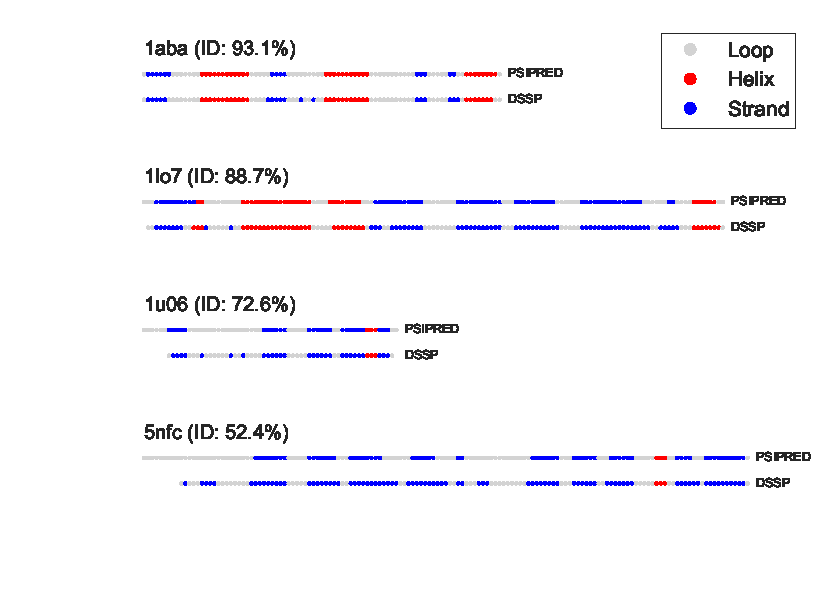
\includegraphics[width=\textwidth]{ample_flib_psipred.pdf}
	\caption[PSIPRED schema for FLIB targets]{Schematic comparison of PSIPRED \cite{Jones1999-ed} secondary structure prediction and DSSP \cite{Frishman1995-si} assignment. Percentage identity is provided next to each identifier. The identity was computing using the Hamming distance over all positions present in the target sequence and reference structure.}
	\label{fig:ample_flib_psipred}
\end{figure}

The contact prediction data for METAPSICOV STAGE 1 and STAGE 2 predictions demonstrate the high precision scores achievable by this algorithm (\cref{table:ample_flib_contact_precision}). In this study, the top contact pairs at cutoffs $L$ and $L/2$ were provided to the FLIB algorithm. All targets have precision scores for both sets of predictions at both cutoff levels of $>0.6$ (\cref{table:ample_flib_contact_precision}). A comparison of the sets of contact pairs shows that only every third (for $L/2$ contacts) or every other (for $L$ contacts) contact pair is shared between both METAPSICOV STAGE predictions highlighting the importance of trialling both when selecting FLIB fragments (Jaccard index in \cref{table:ample_flib_contact_precision}).

\begin{table}[H]
  \centering
  \caption[Contact prediction summary for FLIB targets]{Precision scores for METAPSICOV \cite{Jones2015-vq} STAGE 1 and STAGE 2 contact predictions. Jaccard index calculated for the same $L$-dependent selection of contact pairs between METAPSICOV STAGE 1 and STAGE 2 predictions.}
  \label{table:ample_flib_contact_precision}
  \begin{tabularx}{\textwidth}{X X X X X X X}
      \hline
	  \multirow{2}{*}{\textbf{Target}} & \multicolumn{3}{c}{\textbf{$L/2$ contact pairs}} & \multicolumn{3}{c}{\textbf{$L$ contact pairs}} 	\\ \cline{2-7}
	  							&  	Prec\textsubscript{STAGE 1}	& 	Prec\textsubscript{STAGE 2}	& 	Jaccard 	& 	Prec\textsubscript{STAGE 1} 	& 	Prec\textsubscript{STAGE 2} 	& 	Jaccard	\\
	  \hline
	  1aba						&	0.884	&	0.884	&	0.303	&	0.713	&	0.759	&	0.513		\\
	  1lo7						&	0.857	&	0.957	&	0.308	&	0.738	&	0.837	&	0.446		\\
	  1u06						&	0.839	&	0.806	&	0.378	&	0.710	&	0.787	&	0.459		\\
	  5nfc						&	0.822	&	0.836	&	0.327	&	0.619	&	0.762	&	0.434		\\ 
	  \hline
  \end{tabularx}
\end{table}

Given the two METAPSICOV contact prediction files, both show localised clusters of contact pairs characteristic for secondary structure features (\cref{fig:ample_flib_cmaps}). These clusters are more populated with contact pairs in METAPSICOV STAGE 2 predictions. This behaviour is to-be-expected given that the second stage in METAPSICOV screens the first to remove singleton contact pairs whilst enriching the already existing clusters \cite{Jones2015-vq}. Besides the visual analysis, a cluster determination study on each of those contact maps further confirmed a higher singleton frequency in METAPSICOV STAGE 1 predictions. The latter contain on average 9\% more singleton contact pairs, and thus a higher degree of noise.

\begin{figure}[H]
	\centering
	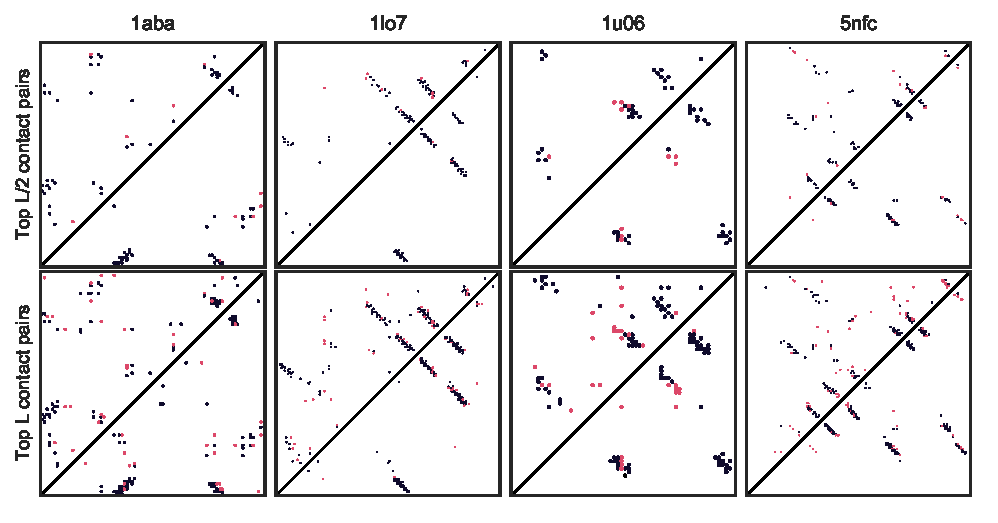
\includegraphics[width=\textwidth]{ample_flib_cmaps.pdf}
	\caption[Contact map comparison for FLIB targets]{Comparison of $L/2$ and $L$ correctly and incorrectly predicted contact pairs for four FLIB targets. Contacts were predicted using METAPSICOV \cite{Jones2015-vq} STAGE 1 (top left) and STAGE 2 (bottom right). True and false positive contact pairs were identified using a 8\AA\ cutoff between C\textalpha\ (C\textbeta\ in case of GLY) atoms of a reference crystal structure. PSIPRED \cite{Jones1999-ed} secondary structure prediction provided along the diagonal.}
	\label{fig:ample_flib_cmaps}
\end{figure}

An analysis of the \gls{mae} of torsion angles between the SPIDER2 \cite{Heffernan2015-bt} prediction and a corresponding reference crystal structure highlights accurate predictions for three of four targets (\cref{fig:ample_flib_spider2}). The largest \gls{mae}\textsubscript{\textphi} across the four target sequences is $24.347^{\circ}$, and the largest \gls{mae}\textsubscript{\textpsi} is $45.459^{\circ}$ (\gls{mae} values for \gls{pdb} entry 1u06). The smallest \gls{mae}\textsubscript{\textphi} is $13.822^{\circ}$ (\gls{pdb} ID: 1aba) and smallest \gls{mae}\textsubscript{\textpsi} is $17.273^{\circ}$ (\gls{pdb} ID: 1lo7). Segments in sequence space with regular secondary structure, as predicted by PSIPRED \cite{Jones1999-ed}, result primarily in low \gls{mae} values of torsion angles. In contrast, unstructured regions highlight much larger \gls{mae} values indicating the difficulty of predicting these regions. Noticeably, the \gls{mae}\textsubscript{\textpsi} appears to be much larger in those regions than the \gls{mae}\textsubscript{\textphi} for the same residue.

In summary, all target sequences have FLIB input data of good quality, which should allow FLIB to select fragments of suitable accuracy for \gls{mr}.

\begin{figure}[H]
	\centering
	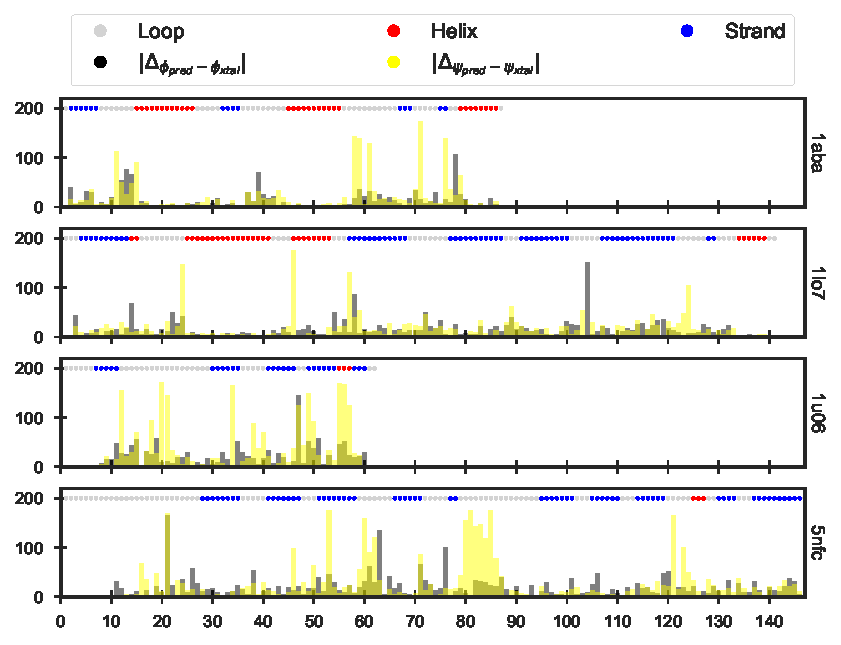
\includegraphics[width=\textwidth]{ample_flib_spider2.pdf}
	\caption[SPIDER2 torsion angle prediction analysis of FLIB targets]{Comparison of \gls{mae} of torsion angles predicted by SPIDER2 and extracted from a corresponding \gls{pdb} structure. PSIPRED \cite{Jones1999-ed} secondary structure prediction provided alongside the \gls{mae} values.}
	\label{fig:ample_flib_spider2}
\end{figure}

\subsection{FLIB fragment picking}
Sixteen FLIB fragment libraries were picked for each protein target in this study. Each fragment library consisted of one permutation of one of two contact prediction files and altering input parameters.

Across all four targets, the FLIB algorithm selected a total of 8,535,458 fragments (\cref{table:ample_flib_frag_summary}). The fragment libraries show similar statistics across the four protein targets despite the diversity in fold and chain lengths. The mean FLIB score is ~3,200 score units with a mean \gls{rmsd} of 9.00\AA. Fragments for the alpha-spectrin SH3 domain (\gls{pdb} ID: 1u06) scored the lowest mean FLIB score with 3,034 units; however, the same target scored the worst by mean \gls{rmsd} with an average of 9.47\AA. In contrast, fragments picked for the sequence of the bacteriophage T4 glutaredoxin (\gls{pdb} ID: 1aba) achieved the best mean \gls{rmsd} of 7.85\AA\ given the second highest mean FLIB score of 3,217 units (\cref{table:ample_flib_frag_summary}).

\begin{table}[H]
  \centering
  \scriptsize
  \caption[FLIB fragment characterics across four protein targets]{Summary of fragment statistics for FLIB libraries selected for four protein targets. Count\textsubscript{H} corresponds to the count of fragments extracted from homologs.}
  \label{table:ample_flib_frag_summary}
  \begin{tabularx}{\textwidth}{X X X X X X X X X}
      \hline
      \multirow{2}{*}{\textbf{Target}} & \multirow{2}{*}{\textbf{Count}} & \multirow{2}{*}{\textbf{Count\textsubscript{H}}} & \multicolumn{3}{c}{\textbf{FLIB score}} & \multicolumn{3}{c}{\textbf{\gls{rmsd}}} \\ \cline{4-9}
      		&			&			& Median 	& Mean 		& Std Dev 	& Median 	& Mean 	& Std Dev \\
      \hline
      1aba	& 2,091,321	& 45,133		& 3,061	& 3,217	& 1,405	& 7.70	& 7.85	& 3.81	\\
	  1lo7	& 2,497,813	& 23,396		& 3,187	& 3,371	& 1,497	& 9.00	& 9.43	& 4.61	\\
      1u06	& 1,133,517	& 60,159		& 2,901	& 3,034	& 1,306	& 9.51	& 9.47	& 3.94	\\
      5nfc	& 2,812,807	& 48,828		& 2,982	& 3,127	& 1,316	& 8.89	& 9.16	& 4.18	\\
      \hline
      Total	& 8,535,458	& 177,516		& 3,049	& 3,208	& 1,397	& 8.68	& 8.96	& 4.25	\\
      \hline
  \end{tabularx}
\end{table}

A split of the per-target fragment libraries by input options highlights the better fragment library quality under certain conditions with regards to the mean FLIB score and \gls{rmsd} (\cref{fig:ample_flib_flibcond}). In particular, top-$L$ (6 residues sequence separation) METAPSICOV STAGE 1 contact predictions yielded the lowest for both metrics across all targets. A comparison of the sequence separation, i.e. using all contact pairs or medium- and long-range ones only, strongly suggests much lower and thus more favourable scores for using short-, medium- and long-range contact pairs. A very similar difference is noticeable for METAPSICOV STAGE 2 contact predictions (\cref{fig:ample_flib_flibcond}). 

\begin{figure}[H]
	\centering
	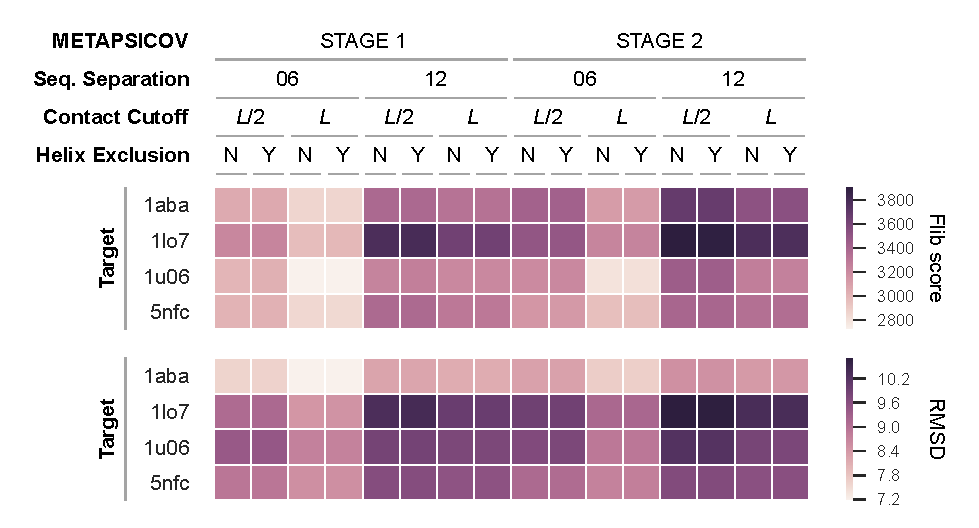
\includegraphics[width=\textwidth]{ample_flib_flibcond.pdf}
	\caption[FLIB fragment library comparison]{FLIB fragment library comparison for four targets highlighting the differences in mean FLIB score and \gls{rmsd} by starting with different subsets of contact predictions. $L$ refers to the number of residues per target sequence. $Y$ refers to idealised \textalpha-helical fragment exclusion during fragment picking; $N$ refers to treating those fragments like all others.}
	\label{fig:ample_flib_flibcond}
\end{figure}

In this study, predicted contact information was used to further guide fragment selection. The FLIB algorithm only selected fragment for positions of the target sequence with at least one contact pair. Given this scenario, an analysis of the coverage of the target sequence with respect to each picking strategy further demonstrates the benefits of starting with METAPSICOV STAGE 1, i.e. noisier contact predictions (\cref{fig:ample_flib_fragtps}). Coverage is more evenly spread across the target sequences compared to missing regions especially for target 4-hydroxybenzoyl CoA thioesterase (\gls{pdb} ID: 1lo7) when starting with METAPSICOV STAGE 2 predictions. Noticeably, none of the picking strategies yielded any fragments for the C-termini of \textalpha-spectrin SH3 domain (\gls{pdb} ID: 1u06) and galectin-3 CRD (\gls{pdb} ID: 5nfc) (\cref{fig:ample_flib_fragtps}). Furthermore, an analysis of the precision of fragments in each library strongly supports the benefits of starting with top-$L$ (6 residues sequence separation) METAPSICOV STAGE 1 contact pairs. Across all four targets, the coverage of correct fragments (classed by \gls{rmsd} $<1.5$\AA\ to the reference structure) is highest for this condition. This is of particular importance for \textalpha-spectrin SH3 domain (\gls{pdb} ID: 1u06) and galectin-3 CRD (\gls{pdb} ID: 5nfc), for which most strategies picked very few to no correct fragments. Excluding idealised \textalpha-helical fragments does not affect the quality of the FLIB libraries greatly. A consideration of differences in mean FLIB and \gls{rmsd} scores shows \textDelta\ differences of 25.68 and 0.06 between the comparable libraries, i.e. with and without idealised \textalpha-helical fragments.

\begin{figure}[H]
	\centering
	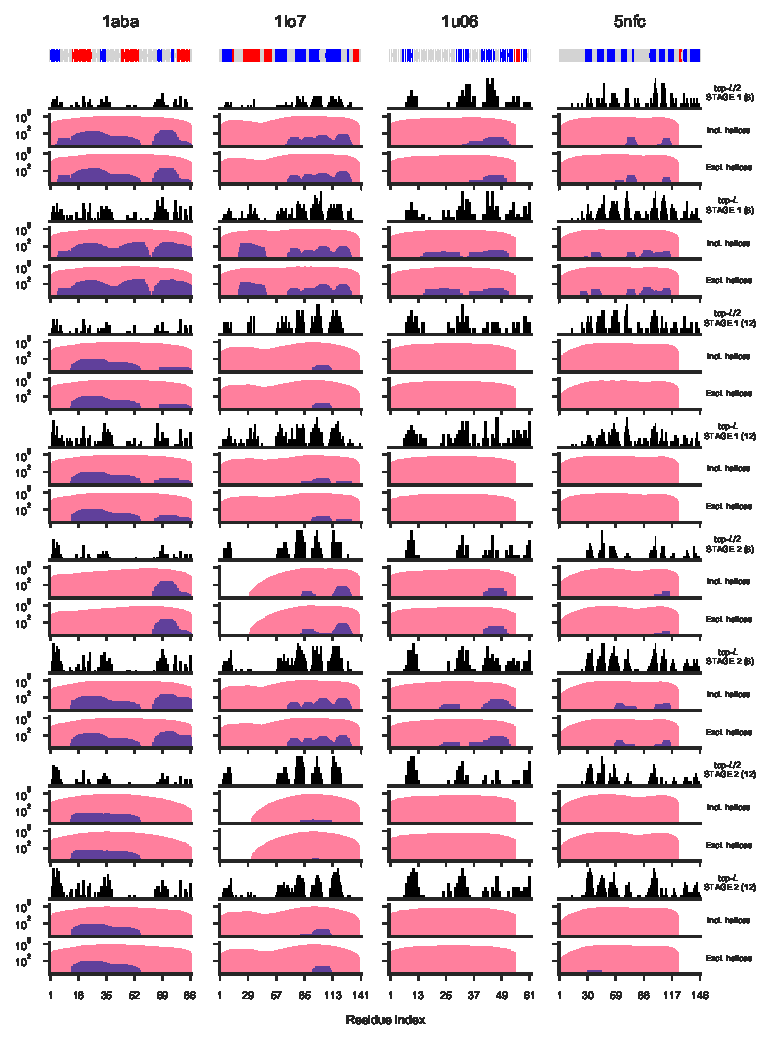
\includegraphics[width=\textwidth]{ample_flib_fragtps.pdf}
	\caption[Coverage and precision of Flib fragment libraries]{Summary of the coverage and precision of FLIB fragment libraries according to their target sequence. The coverage of all fragments with respect to their target-aligned sequence register are shown in red bars, and fragments with \gls{rmsd} $<1.5$\AA\ to the reference structure in blue. The predicted secondary structure of each target sequence is given at the top: \textalpha-helices (red), \textbeta-strands (blue), and loops (gray). Contact prediction information is illustrated using black bars. The fragment frequency is shown using a log-scale.}
	\label{fig:ample_flib_fragtps}
\end{figure}

Given that FLIB uses co-evolution data to help select fragments, it is little surprise that higher degrees of \gls{tp} fragments co-localise with high-density contact pair regions along the target sequence (\cref{fig:ample_flib_fragtps}). This characteristic explains less \gls{tp} fragments in top-$L/2$ fragment libraries because less contacts (compared to top-$L$) are available during fragment selection. The resulting selection is purely based on the FLIB score which might not yield high-accuracy fragments (\gls{rmsd} $<1$\AA) as frequently. Therefore, the co-localisation of \gls{tp} FLIB fragments and regions of high-density contact predictions highlights the importance of adding this additional source of information to pick fragments. 

\subsection{FLIB fragment selection for Molecular Replacement}
One of the most important aspects of bypassing \textit{ab initio} structure prediction and using the relevant fragments directly as \gls{mr} search models is the selection of the fragments with the highest similarity between fragment and target structure.

A fragment's FLIB score --- its cumulative absolute error of predicted torsion angles --- has the highest correlation with the \gls{rmsd} of a fragment compared to all other scores used in the FLIB protocol \cite{De_Oliveira2015-kb}. To validate this finding, all non-homologous fragments in this study were tested for a correlation between a their FLIB scores and \gls{rmsd} values. The Spearman's rank-order correlation coefficient analysis confirms the correlation between a fragment's FLIB and \gls{rmsd} scores (\cref{fig:ample_flib_flibspearman}). However, the strength of the correlation varies greatly between different fragment libraries and targets. The optimal fragment picking strategy --- top-$L$ (6 residues sequence separation) METAPSICOV STAGE 1 --- results in the strongest correlations across all targets. The same contact pair selection with METAPSICOV STAGE 2 predictions results in the second greatest correlations. Noticeably, the bacteriophage T4 glutaredoxin (\gls{pdb} ID: 1aba) fragment libraries show much more positive correlations than the remaining targets. The fragments selected for \textalpha-spectrin SH3 domain (\gls{pdb} ID: 1u06) show the overall weakest correlations. It is worth noting that the both targets, \gls{pdb} IDs 1aba and 1lo7, are classed as mixed \textalpha-\textbeta\ targets, and thus the strength of this correlation might be fold dependent.

\begin{figure}[H]
	\centering
	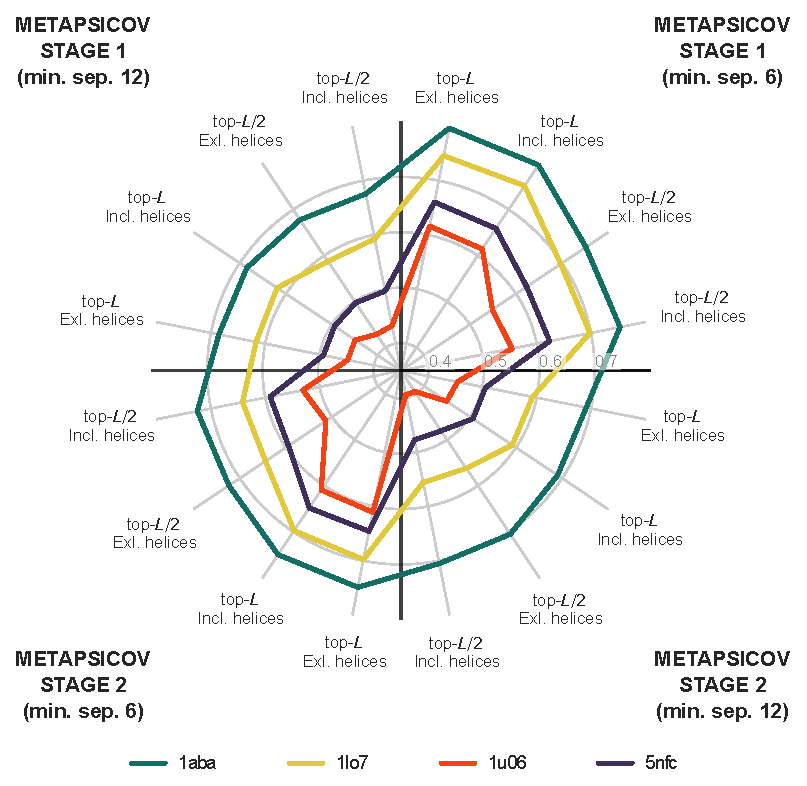
\includegraphics[width=\textwidth]{ample_flib_flibspearman.pdf}
        \caption[Spearman rank-order correlation coefficient analysis of FLIB fragments]{Spearman rank-order correlation coefficient analysis of FLIB fragments' FLIB score and \gls{rmsd} value given the 16 unique fragment picking strategies across four targets. P-values of all Spearman correlations are $<0.001$ and not shown for simplicity of the plot.}
	\label{fig:ample_flib_flibspearman}
\end{figure}

Further inspection of the fragments and the relationship between each fragment's FLIB score and \gls{rmsd} value reveals a small subset of outliers in each fragment library. These fragments (hereafter referred to as outlier fragments) are sparse in each library with an overall mean count of $<0.2$\%. An analysis for unique characteristics of these outliers, which would allow for their exclusion, reveals no unique feature. These fragments contain all secondary structure types, span the entire target sequence and range over all peptide lengths. Furthermore, they occur in all fragment libraries, irrelevant of their original picking strategy. The only characteristic setting these outlier fragments apart from the remaining set is a \gls{rmsd} value of $>30$\AA. Nevertheless, it appears that these outlier fragments with unusually high \gls{rmsd} values are never included in the final fragment search model set, given that their overall FLIB\textsubscript{min} score is 796 units (one order of magnitude more than the overall minimum for the remaining fragments).

An analysis of the fragment metrics in the final \gls{mr} set (6,547 fragments) further supports the positively linear relationship between a fragment's FLIB score and \gls{rmsd} (\cref{fig:ample_flib_finalrelat}a). However, the best FLIB fragments by \gls{rmsd} show much less spread compared to the best fragments by FLIB score (\cref{fig:ample_flib_finalrelat}b). Furthermore, the size of the fragments also positively correlates with the the FLIB ($\rho_{Spearman}=0.860$, $p<0.001$) and \gls{rmsd} ($\rho_{Spearman}=0.697$, $p<0.001$) values. Longer fragments with higher dissimilarity with respect to the target show higher FLIB scores and \gls{rmsd} values (\cref{fig:ample_flib_finalrelat}a). 

\begin{figure}[H]
	\centering
	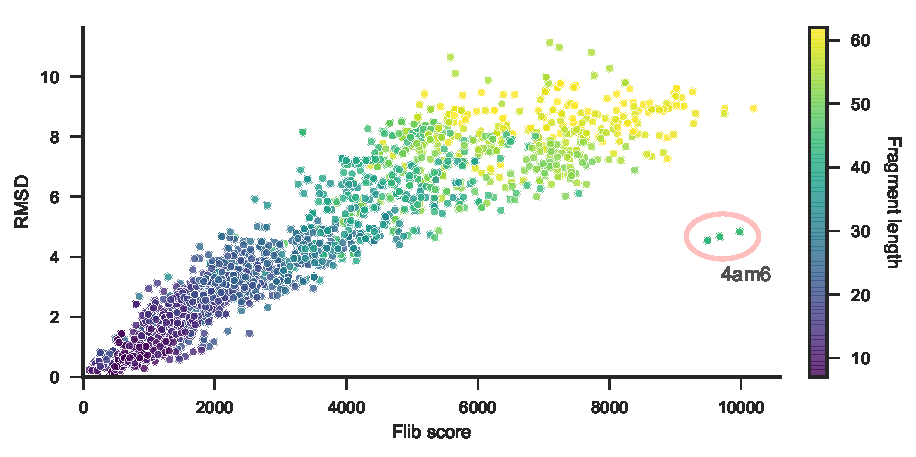
\includegraphics[width=\textwidth]{ample_flib_finalrelat.pdf}
        \caption[Correlation analysis for final FLIB \gls{mr} fragments]{Scatterplot highlighting the positive correlation between fragment FLIB scores and \gls{rmsd} values. The plot contains all fragments independent of target or picking strategy. \textbf{a.} The colour of each scatter point illustrates the fragment length. All extreme outlier fragments are highlighted with their \gls{pdb} identifiers as labels. \textbf{b.} The colour codes indicate the sorting strategy to select the top FLIB fragments for each fragment peptide length bin.}
	\label{fig:ample_flib_finalrelat}
\end{figure}

Notably, a cluster of large fragments with some of the highest FLIB scores in the set show a reasonable similarity to their target structure (\cref{fig:ample_flib_finalrelat}a). All fragments in this cluster were picked for the bacteriophage T4 glutaredoxin sequence (\gls{pdb} ID: 1aba) and extracted from the same region of the crystal structure of the actin-related protein ARP8 (\gls{pdb} ID: 4am6). In comparison, some smaller fragments with peptide lengths $<50$ residues and lower FLIB scores of $<3000$ show the highest \gls{rmsd} values in the final set.

One further unique aspect of this study compared to other fragment-\gls{mr} approaches is the use of residue-residue contact information to select fragments during picking, only selecting fragments for target-sequence residues with at least one contact pair in the predicted set (Saulo de Oliveira, personal communication). In the final set 39\% of all fragments satisfy at least one, 26\% at least two and 20\% at least three contact pairs. Across the four targets, 50\% of all fragments selected for 4-hydroxybenzoyl CoA thioesterase (\gls{pdb} ID: 1lo7) satisfy at least one predicted contact pair (\cref{fig:ample_flib_consatis}). In comparison, 28\% of fragments selected for the \textalpha-spectrin SH3 domain (\gls{pdb} ID: 1u06) satisfy at least one contact pair.

\begin{figure}[H]
	\centering
	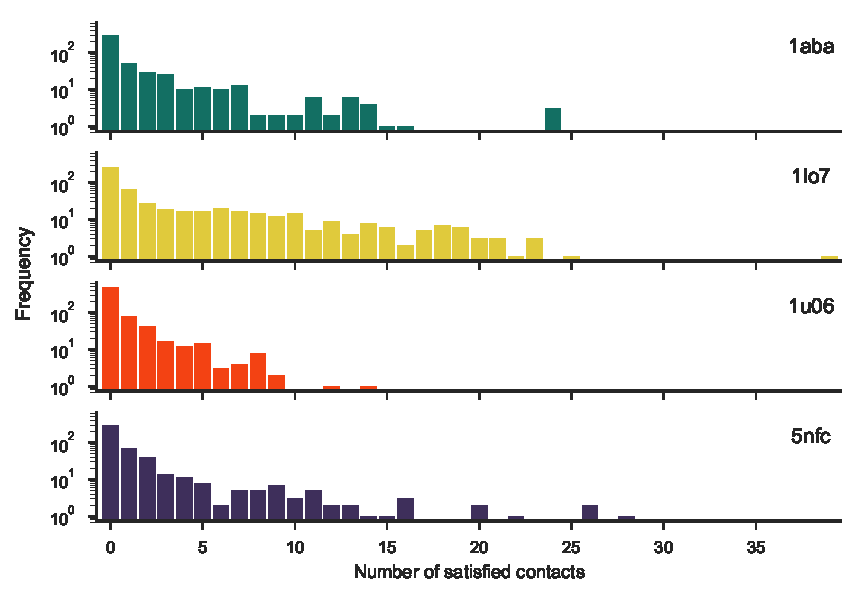
\includegraphics[width=\textwidth]{ample_flib_consatis.pdf}
	\caption[Distribution of contact precision for FLIB fragments]{Distribution of contact precision for FLIB fragments selected as \gls{mr} search models separated on a per-target basis.}
	\label{fig:ample_flib_consatis}
\end{figure}

Thus, the final set of FLIB fragment \gls{mr} search models spans a wide range of peptide lengths, \gls{rmsd} values, contact precision scores, and generally secondary structure make-up. To illustrate the latter, a random selection of sample fragments is illustrated in \cref{fig:ample_flib_search_models}. Importantly, not a single super-secondary structure motif dominates the set, increasing the sampling diversity to be undertaken during \gls{mr}.

\begin{figure}[H]
	\centering
	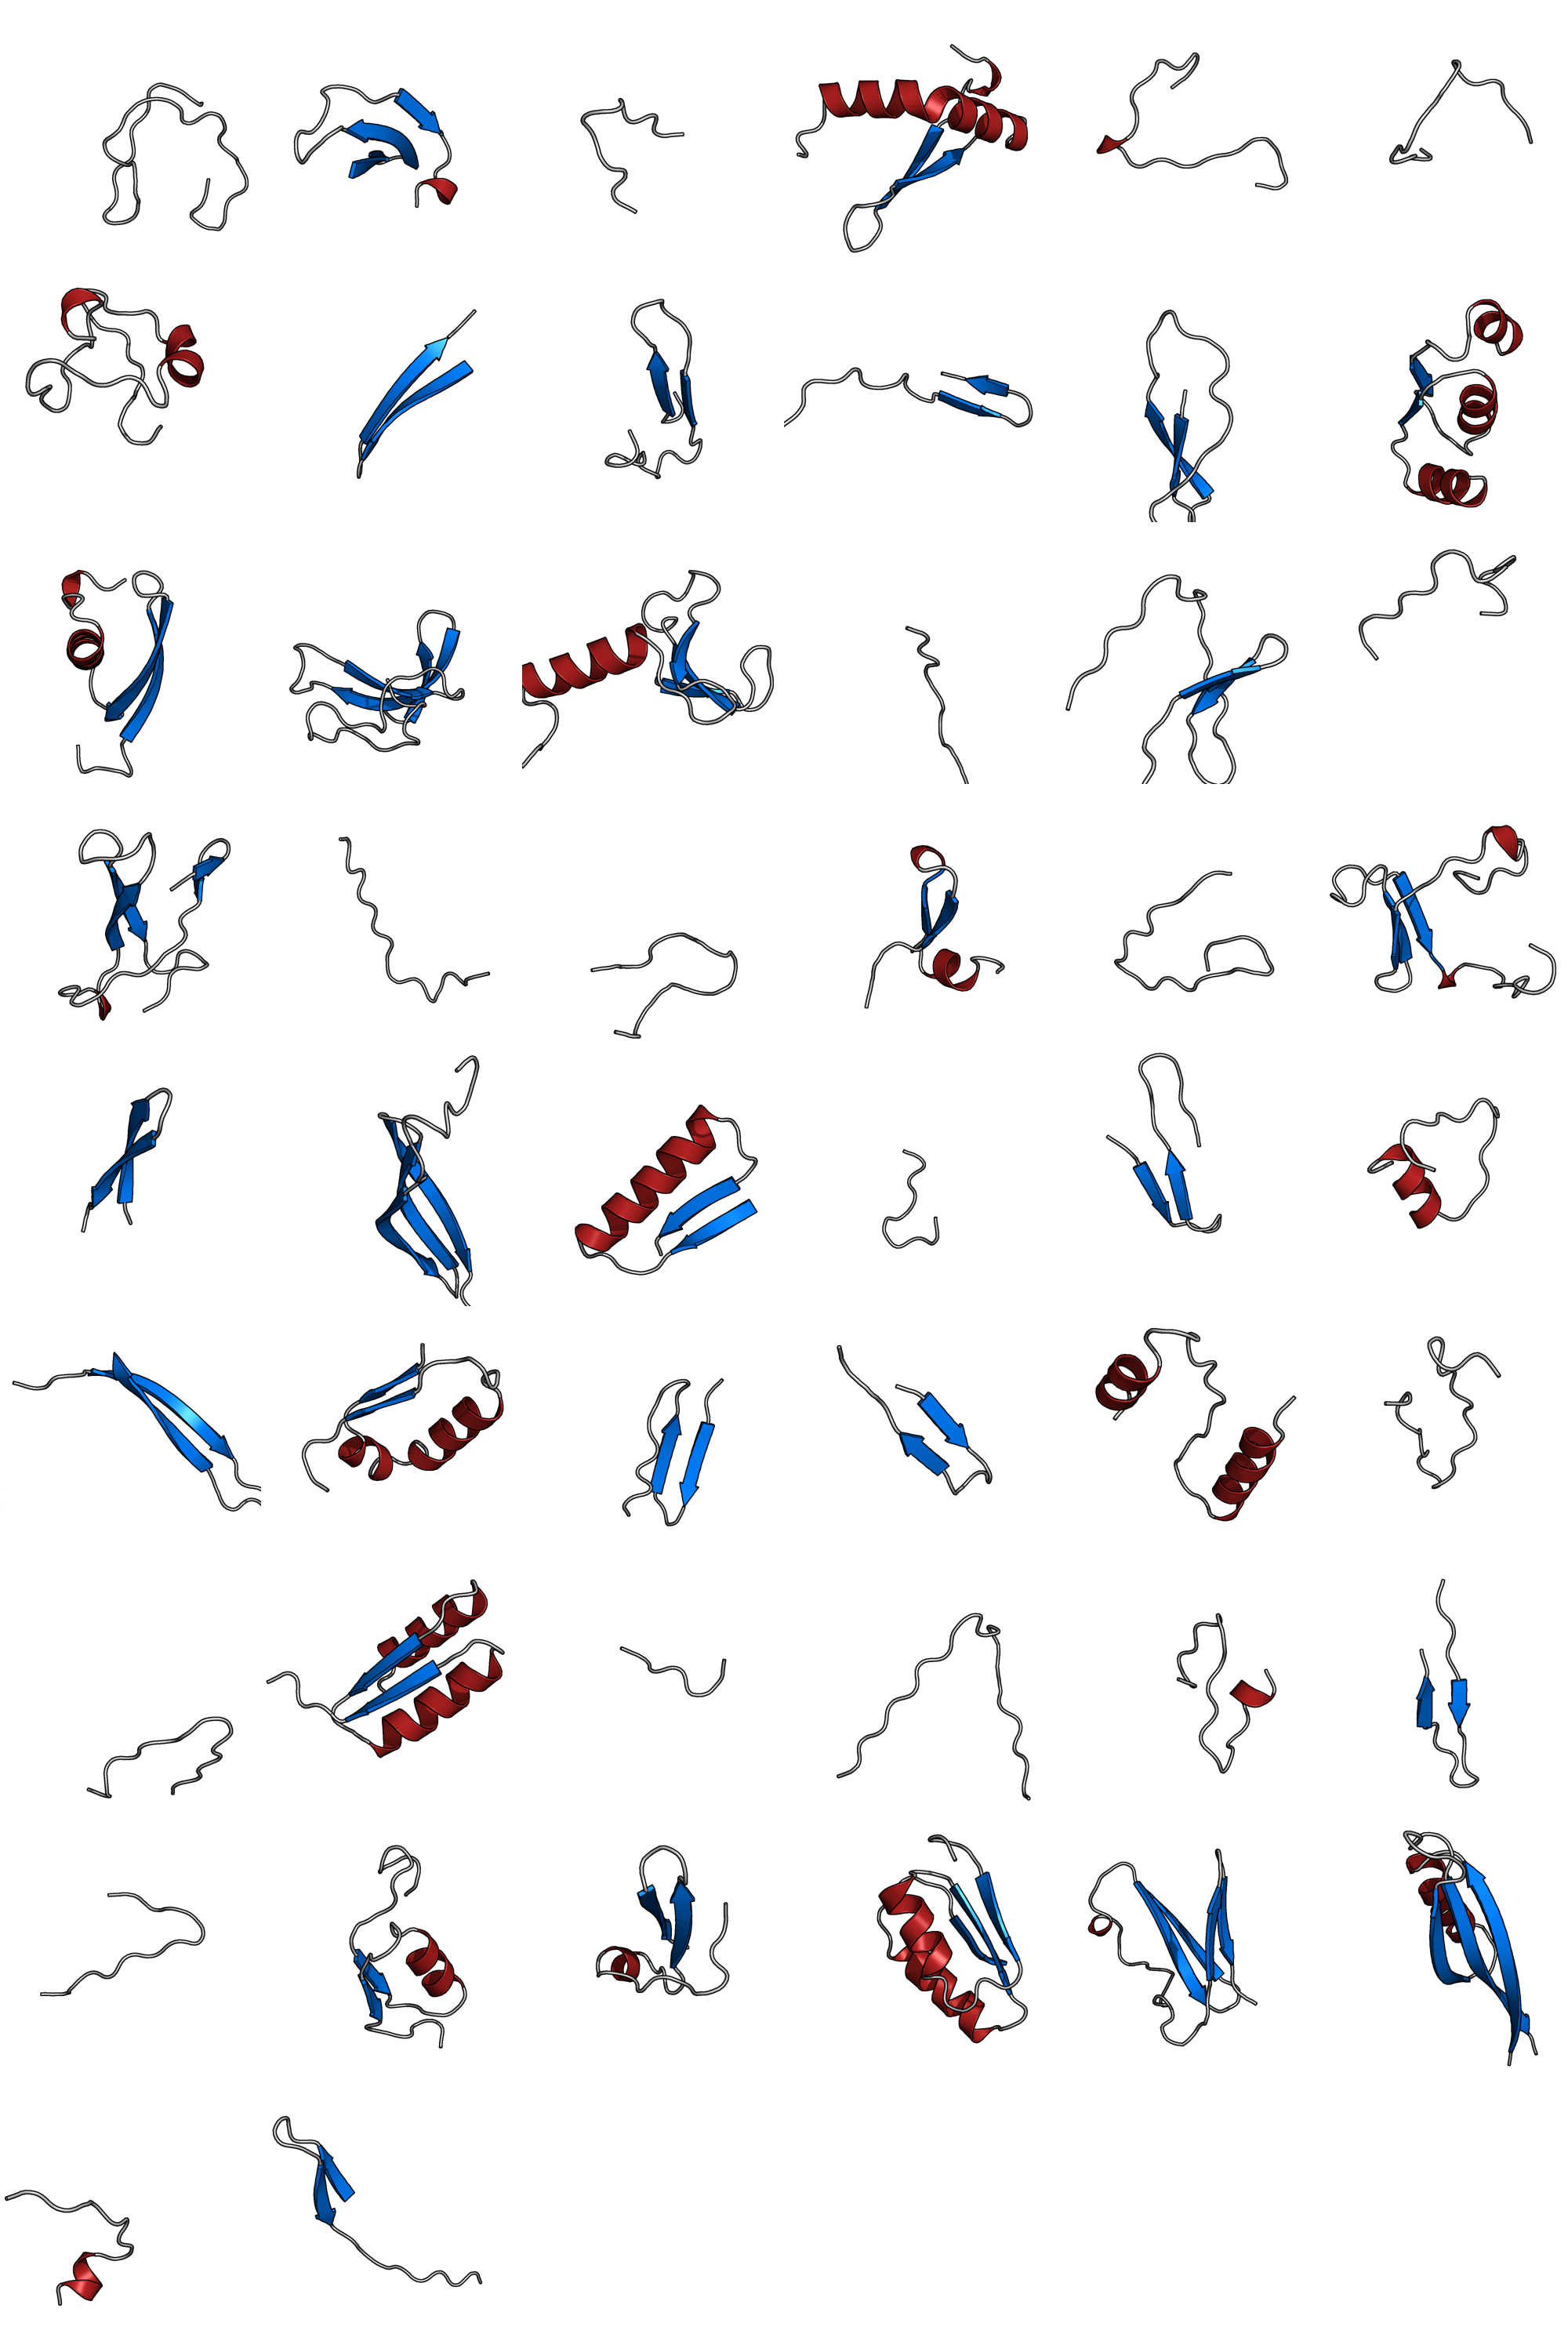
\includegraphics[width=\textwidth]{ample_flib_search_models2.png}
	\caption[Fragment search models derived from FLIB]{Non-redundant sample of FLIB fragment search models selected for four different protein targets. Secondary structure defined by and visualisation done in PyMOL \cite{DeLano2002-hm}. Unpaired \textbeta-strands rendered using the loop style.}
	\label{fig:ample_flib_search_models}
\end{figure}

\subsection{Molecular Replacement using FLIB fragments}
FLIB fragments picked for four target sequences using a variety of FLIB input options generated $>6,500$ fragments, which were subjected to the \gls{mr} pipeline MRBUMP with their corresponding target experimental data. Given that each fragment was trialled with three different PHASER \gls{rmsd} values, a total of 19,716 \gls{mr} attempts were made across four target structures. Out of nearly 20,000 \gls{mr} attempts, 299 led to the structure solutions of two targets, namely the T4 glutaredoxin (\gls{pdb} ID: 1aba) and \textalpha-spectrin SH3 domain (\gls{pdb} ID: 1u06) (\cref{fig:ample_flib_mrsummary}).

\begin{figure}[H]
	\centering
	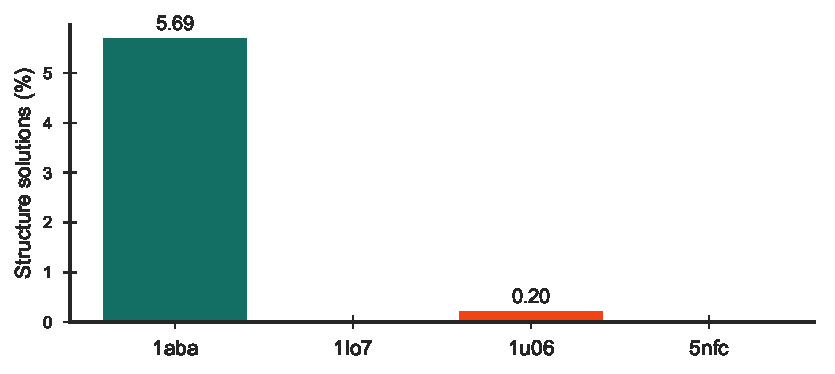
\includegraphics[width=\textwidth]{ample_flib_mrsummary.pdf}
	\caption[MR structure solutions by FLIB target]{Distribution of structure solutions by FLIB target. All \gls{mr} attempts total to 19,716, out of which 299 are structure solutions. Values above each bar indicates percentage search models successful out of the corresponding set.}
	\label{fig:ample_flib_mrsummary}
\end{figure}

The total of 299 \gls{mr} structure solutions were achieved by 70 sequence-unique fragments. Sixty-nine of those fragments were picked from 60 unique structures for the T4 glutaredoxin (\gls{pdb} ID: 1aba) leading to 97\% of all structure solutions. In comparison, a single fragment, selected from three different fragment libraries, led to 9 structure solutions of the \textalpha-spectrin SH3 domain (\gls{pdb} ID: 1u06). The largest FLIB fragment leading to a structure solution contained 37 residues and the smallest 10.

A division of FLIB-fragment search models by their respective origin libraries provides strong evidence that METAPSICOV STAGE 1 contact predictions allows for the selection of the most accurate fragments (\cref{fig:ample_flib_flibcond}), which directly translates into the structure solution count (\cref{fig:ample_flib_flibcondmr}). Furthermore, this division also highlights and supports the quality of fragment libraries picked with top-$L$ (6 residues sequence separation) METAPSICOV STAGE 1 predictions. Trialling the optimal fragment picking strategy with and without helical fragments ($>90$\% \textalpha-helical content assigned using DSSP) resulted in the library without outperforming the other (\cref{fig:ample_flib_flibcondmr}, 3\textsuperscript{rd} and 4\textsuperscript{th} bars). 

\begin{figure}[H]
	\centering
	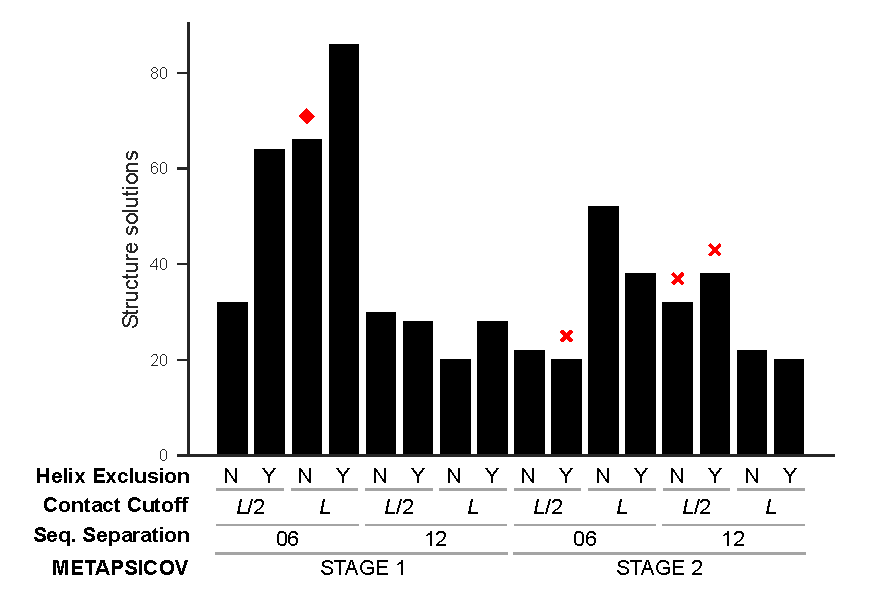
\includegraphics[width=\textwidth]{ample_flib_flibcondmr.pdf}
	\caption[MR structure solutions by FLIB library]{Distribution of structure solutions by FLIB library configuration. The optimal fragment picking strategy, as assessed by FLIB values, is highlighted with a red diamond to illustrate that the method that picks the best fragments is close to, but not the absolute best for ultimate structure solution. Fragment picking strategies leading to solutions of \textalpha-spectrin SH3 domain (\gls{pdb} ID: 1u06) are highlighted with red crosses.}
	\label{fig:ample_flib_flibcondmr}
\end{figure}

An analysis of the binned results by fragment-ranking or PHASER \gls{rmsd} value confirms the expected outcome: the top fragments selected by fragment \gls{rmsd} score result in more structure solutions than their FLIB score counterparts (\cref{fig:ample_flib_mrbyconfig}). To reiterate, all FLIB fragments were grouped by their peptide length, and the top fragment in each group selected when sorted by either FLIB or \gls{rmsd} values. When separating the total number of structure solutions by the score that made each fragment the best in its original library, it becomes clear that two-thirds of solutions were achieved with fragments scoring best by \gls{rmsd}. However, the structure of \textalpha-spectrin SH3 domain (\gls{pdb} ID: 1u06) was only solved with fragments that scored best in their FLIB fragment libraries by FLIB score. A further subdivision of successful fragments, sorted either by FLIB scores or \gls{rmsd} values, highlights that a larger proportion of successful \gls{rmsd}-sorted fragments satisfied at least 1 contact (FLIB-sorted: 7\%; \gls{rmsd}-sorted: 13\%). A separation of attempts by PHASER input \gls{rmsd} value suggests a value of 0.1 to be the most favourable.

\begin{figure}[H]
	\centering
	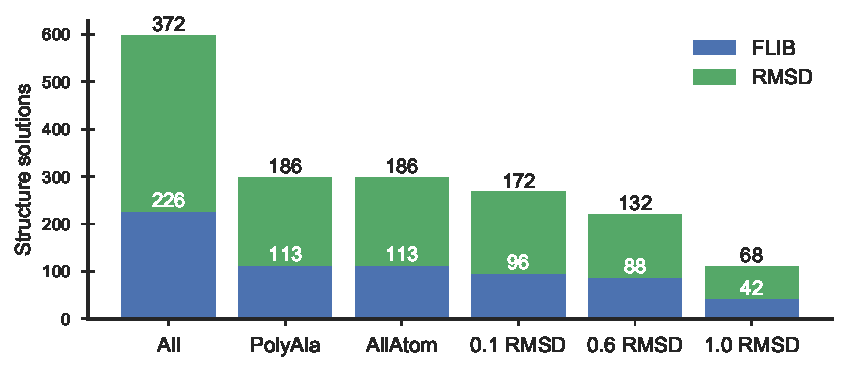
\includegraphics[width=\textwidth]{ample_flib_mrbyconfig.pdf}
	\caption[MR structure solutions by input parameters]{Distribution of structure solutions by fragment and MRBUMP configuration. The structure solution count is provided above each bar.}
	\label{fig:ample_flib_mrbyconfig}
\end{figure}

In \gls{mr}, the correct placement of very small structural fragment may not always be detectable by the output metrics of underlying software. In benchmarking exercises, the \gls{rio} metric has shown to be a very useful and powerful metric to detect such situations \cite{Thomas2015-wu,Thomas2017-sh}. Given that the peptide lengths of FLIB fragments in this study range from 6 to 63 residues, the \gls{rio} score is most suitable in validating the correct placement of FLIB-fragment search models. Indeed, all fragments with SHELXE \gls{cc} $\geq25$ and \gls{acl} $\geq10$ contain at least 3 correctly placed C\textalpha\ atoms (i.e. a \gls{rio} score $\geq3$). Furthermore, the \gls{rio} metric indicates that more than 500 fragments have C\textalpha\ atoms placed within 1.5\AA\ of any atom in the target structure. However, only 4 residues are on average placed correctly, which was not enough to achieve structure solution (\cref{fig:ample_flib_mrrionorm}). All successful FLIB fragments have a minimum model- and target-normalised \gls{rio} scores of 29.7\% and 9.2\% (\cref{fig:ample_flib_mrrionorm}, green markers). 

\begin{figure}[H]
	\centering
	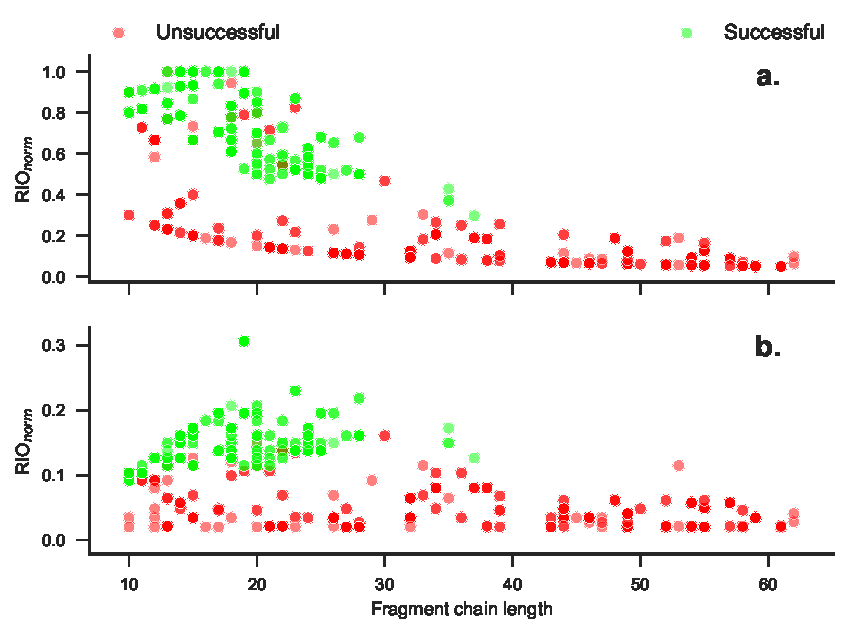
\includegraphics[width=\textwidth]{ample_flib_mrrionorm.pdf}
	\caption[Relationship between fragment chain length and normalised RIO scores.]{Dependence of normalised \acrlong{rio} (RIO\textsubscript{norm}) score on the fragment chain length. The two plots show  \gls{rio} scores normalised by the chain lengths of (a) the fragment and (b) the target. Colour coding indicates if the FLIB-fragment search model resulted in a structure solution. Each plot contains 890 fragment points; however, not all points are visible due to the superposition of individual scatter points because the same fragment was scored under different \gls{mr} conditions.}
	\label{fig:ample_flib_mrrionorm}
\end{figure}

In 33 \gls{mr} attempts more than 60\% of a fragment's residues were placed correctly, yet structure solution was not achieved. These trials affect exclusively fragments picked for the target sequences of T4 glutaredoxin (\gls{pdb} ID: 1aba) and 4-hydroxybenzoyl CoA thioesterase (\gls{pdb} ID: 1lo7). Overall, the 33 \gls{mr} attempts made were done with 17 fragments extracted from 15 templates containing between 10 and 23 amino acids. The fragments' \gls{rmsd} values range from 0.19 to 2.72\AA\ with a mean \gls{rmsd} of 1.10\AA. Surprisingly, almost all of these fragments contain primarily \textalpha-helices. Given the presence of helices in the fold of both targets (\cref{fig:ample_flib_psipred}) and the success of idealised fragments to solve such targets with data resolution $<2.0$\AA, it is a surprise to not see more structure solutions from these fragments.

Finally, the co-evolution data used in this study select fragments is a novelty in the field. Thus, it is of great interest to identify if fragments leading to structure solution satisfy many predicted residue-residue contacts. Eighty-seven percent ($n=61$) of all unique fragments leading to structure solutions for either target satisfy no predicted residue-residue contact. The remaining nine fragments, all of which lead to structure solutions of T4 glutaredoxin (\gls{pdb} ID: 1aba), satisfy either one ($n=4$), two ($n=4$) or 24 ($n=1$) predicted contacts. 

\begin{figure}[H]
	\centering
	\includegraphics[width=\textwidth]{ample_flib_mrchelatase.pdf}
	\caption[Example of FLIB fragment to MR solution]{Intermediary steps from donor structure to SHELXE main-chain autotrace for a fragment derived from cobalt chelatase found in \textit{Salmonella typhimurium} (\gls{pdb} ID: 1qgo). The structure solution was obtained against the target crystallographic data of T4 glutaredoxin (\gls{pdb} ID: 1aba). METAPSICOV STAGE 2 predicted contacts, against which the fragment was selected, are illustrated with \acrlong{tp} (green) and \acrlong{fp} (red) contacts (distance cutoff of 8\AA). 2mFo-DFc electron density maps shown at 2.0 sigma and radius around the peptide atoms of 5\AA. The \gls{rmsd} between the sequence-independently superposed structures of target and donor is 10.384\AA\ (computed with the \texttt{super} command in PyMOL \cite{DeLano2002-hm}).}
	\label{fig:ample_flib_mrchelatase}
\end{figure}

The fragment with 24 satisfied contacts is a particularly striking example of the value of the approach explored in this study (\cref{fig:ample_flib_mrchelatase}). The fragment was derived from the template structure of cobalt chelatase found in \textit{Salmonella typhimurium} (\gls{pdb} ID: 1qgo). The picked fragment contains 35 residues and its supersecondary structure consists of a two-strand \textbeta-sheet packing against a single \textalpha-helix. The majority of satisfied contact pairs are between C\textbeta\ atoms of the \textbeta-strands; however, a small number of individual contact pairs also identifies the packing of one \textbeta-strand against the \textalpha-helix (\cref{fig:ample_flib_mrchelatase}, top-right). Although not considered at this stage in the FLIB algorithm, this particular fragment satisfies 75\% of all relevant contact pairs. Most importantly though, this fragment was derived from an entirely unrelated protein structure, and thus illustrated the value in \textit{ab initio} structure prediction fragments as \gls{mr} search models.

\section{Discussion}
The main objective of this study was to investigate the application of FLIB structural fragments to \gls{mr}. Four experimental datasets were chosen and 16 FLIB fragment libraries built per target sequence varying primarily in the predicted residue-residue contact information. A selection of highest scoring fragments were then forwarded to MRBUMP to trial each fragment as \gls{mr} search model. The findings in this study validate the concept of this approach. Firstly, a positive correlation between a fragment's FLIB score and \gls{rmsd} value was identified. These correlations were target-independent and found, with various strengths, in all FLIB fragment libraries. Furthermore, this work has identified top-$L$ (6 residue sequence separation) METAPSICOV STAGE 1 contact pairs to be the optimal selection of contact pairs for the FLIB algorithm when starting with METAPSICOV predictions. The additional noise, typically filtered in the second STAGE of the METAPSICOV algorithm \cite{Jones2015-vq}, allowed for the selection of more accurate fragments across the entire target sequence. Lastly, trialling a selection of high-scoring FLIB fragments in routine \gls{mr} showed the usefulness of such fragments in attempting to solve protein structures. Two out of four targets were successfully solved albeit only trialling a small proportion of FLIB fragments per library (mean MRBUMP runtime of 10.5 CPU hours per fragment).

Intuitively, most crystallographers would declare the limitations of this approach to be the size and quality of the selected FLIB fragments as well as the resolution of the crystallographic data. Although the former was long-thought to be a major limitation, more recent work highlighted the success of likelihood-based \gls{mr} methods (i.e., PHASER \cite{McCoy2007-mp}) with very small search models. \textcite{McCoy2017-cz} demonstrated the successful \textit{ab initio} \gls{mr} structure solution of aldose reductase starting from as little as two correctly placed atoms. Furthermore, automated \gls{mr} pipelines, such as AMPLE \cite{Bibby2012-lm}, ARCIMBOLDO \cite{Rodriguez2012-ad}, BORGES \cite{Sammito2013-ug}, FRAGON \cite{Jenkins2018-gf} or FRAP \cite{Shrestha2015-zb}, also successfully demonstrated \gls{mr} successes with search models comprising a fraction of the target structure. Thus, \gls{mr} structure solutions with FLIB fragments as short as 6 residues should be considered possible, especially when high resolution data is available and the fragment size is proportionally large compared to target size.

\Gls{mr} search models need to be sufficiently accurate to derive phase information for successful structure solution. The findings in this study highlight the success of identifying accurate fragments solely by the fragment's FLIB score. Given that the FLIB implementation used in this study only selected fragments for positions with at least one available contact pair, future research is required to identify the potential benefits of specifically selecting fragments that satisfy at least one contact pair. Furthermore, it is important to understand the potentially beneficial implications of using the contact satisfaction score in the FLIB score metric of a given fragment. In theory, higher precision scores should imply a closer match of the overall tertiary structure of the trialled region. Alternatively, selecting secondary structure motifs or substructures of templates by means of searching with a predicted contact map could be an attractive alternative. Recent studies indicated success in identifying sub-folds by means of \gls{cmo} \cite{Buchan2017-ox,Ovchinnikov2017-nd}. Further work also needs to explore the benefits of considering the \gls{ellg} as a conceptual framework to identify the linked effects of the fragment search model size, its accuracy and the resolution on the solvability of a target structure \textcite{McCoy2017-cz}.

Nevertheless, FLIB fragments with near-identical subfolds to the target might not be traceable by current means of assessing structure solutions. Commonly, \gls{mr} success is judged by the combination of SHELXE \gls{cc} and \gls{acl} scores \cite{Thorn2013-le}. However, it is known that \textbeta-strands are notoriously difficult to trace, and thus SHELXE might not pick up on correctly placed search models. Although this study did not suffer from this problem for fragments containing primarily \textbeta-strands, it did have correctly placed \textalpha-helices without structure solutions. Thus, the approach taken in this study would benefit from improvements to the density modification and sequence tracing algorithms.

Finally, this work served primarily as proof-of-concept study, and thus attempted to explore a diversity of options. With a better understanding of input parameters future work could build on the work presented here and use a large-scale analysis to assess the suitability of this concept more thoroughly. Furthermore, improvements to the FLIB algorithm through the incorporation of co-evolution data should also improve the quality of \textit{ab initio} structure predictions, which should result in a greater success rate of other \gls{mr} pipelines, such as AMPLE \cite{Bibby2012-lm}.


% \chapter{Conclusion}

% \appendix
% \chapter{Appendix Title}
% 
\begin{sidewaystable}
    \footnotesize
    \centering
    \caption{Summary of the ORIGINAL dataset.}
    \label{table:appendix_dataset_original}
    \begin{tabularx}{\textheight}{ t b t t t t t t t s t }
        \hline
        \textbf{\gls{pdb} ID} & \textbf{Molecule}	& \textbf{Resolution (\AA)}	& \textbf{Space Group}	& \textbf{Chain ID}	& \textbf{Chain Length}	& \textbf{Molecules per ASU}	& \textbf{Matthew's Coefficient}	& \textbf{Solvent Content (\%)}	& \textbf{Fold}	& \textbf{Citation}	\\
        \hline
        1a6m		&	Oxy-myoglobin											&	1.00		&	P$2_1$			& A	&	151	&	1	&	1.90		&	36.00	&	all-\textalpha				& \cite{Vojtechovsky1999-nn}	\\
        1aba		&	T4 glutaredoxin											&	1.45		&	P$2_1 2_1 2_1$	& A	&	87	&	1	&	2.22		&	44.62	&	mixed \textalpha/\textbeta	& \cite{Eklund1992-gz}			\\
        1bdo		&	Biotinyl domain of acetyl-coenzyme A carboxylase		&	1.80		&	P$2_1 2_1 2$	& A	&	80	&	1	&	2.48		&	49.00	&	all-\textbeta				& \cite{Athappilly1995-yu}		\\
        1bkr		&	Calponin Homology (CH) domain from \textbeta-spectrin	&	1.10		&	P$2_1$			& A	&	109	&	1	&	2.04		&	39.80	&	all-\textalpha				& \cite{Banuelos1998-jk}		\\
        1chd		&	CheB methylesterase domain								&	1.75		&	P$3_2 2 1$		& A	&	203	&	1	&	2.35		&	47.65	&	mixed \textalpha/\textbeta	& \cite{West1995-dp}			\\
        1e0s		&	G-protein Arf6-GDP										&	2.28		&	P$6_1 2 2$		& A	&	174	&	1	&	2.18		&	37.00	&	mixed \textalpha/\textbeta	& \cite{Menetrey2000-nw}		\\
        1eaz		&	Phosphoinositol (3,4)-bisphosphate PH domain			&	1.40		&	C$2 2 2_1$		& A	&	125	&	1	&	2.48		&	48.00	&	mixed \textalpha+\textbeta	& \cite{Thomas2001-uf}			\\
        1hh8		&	N-terminal region of P67Phox							&	1.80		&	P$3_1$			& A	&	213	&	1	&	2.71		&	45.00	&	all-\textalpha				& \cite{Grizot2001-ju}			\\
        1kjl		&	Galectin-3 domain										&	1.40		&	P$2_1 2_1 2_1$	& A	&	146	&	1	&	2.15		&	42.68	&	all-\textbeta				& \cite{Sorme2005-ln}			\\
        1kw4		&	Polyhomeotic SAM domain									&	1.75		&	P$6_5$			& A	&	89	&	1	&	2.25		&	45.27	&	all-\textalpha				& \cite{Kim2002-vg}				\\
        1lo7		&	4-hydroxybenzoyl CoA thioesterase						&	1.50		&	I$2 2 2$		& A	&	141	&	1	&	2.06		&	40.22	&	mixed \textalpha+\textbeta	& \cite{Thoden2002-id}			\\
        1npu		&	Extracellular domain of murine PD-1						&	2.00		&	P$2_1 2_1 2_1$	& A	&	117	&	1	&	1.67		&	25.80	&	all-\textbeta			& \cite{Zhang2004-zt}			\\
        1pnc		&	Poplar plastocyanin										&	1.60		&	P$2_1 2_1 2_1$	& A	&	99	&	1	&	1.82		&	32.48	&	all-\textbeta				& \cite{Fields1994-zx}			\\
        1tjx		&	Synaptotagmin I C2B domain								&	1.04		&	P$3_2 2 1$		& A	&	159	&	1	&	2.40		&	48.00	&	mixed \textalpha+\textbeta	& \cite{Cheng2004-es}			\\
        1tlv		&	LicT PRD												&	1.95		&	P$3_2 2 1$		& A	&	221	&	1	&	2.80		&	50.00	&	all-\textalpha				& \cite{Graille2005-at}			\\
        2nuz		&	\textalpha-spectrin SH3 domain							&	1.85		&	P$2_1 2_1 2_1$	& A	&	62	&	1	&	2.57		&	52.16	&	all-\textbeta				&								\\
        2qyj		&	Ankyrin													&	2.05		&	P$6_1$			& A	&	166	&	1	&	2.28		&	45.99	&	all-\textalpha				& \cite{Merz2008-aa}			\\
        3w56		&	C2 domain					 							&	1.60		&	I$2$			& A	&	131	&	1	&	2.05		&	40.10	&	all-\textbeta				& \cite{Traore2013-ul}			\\
        4cl9		&	N-terminal bromodomain of Brd4							&	1.40		&	P$2_1 2_1 2_1$	& A	&	127	&	1	&	2.21		&	44.37	&	all-\textalpha				& \cite{Atkinson2014-he}		\\
        4u3h		&	FN3con													&	1.98		&	P$4_1 3 2$		& A	&	100	&	1	&	2.47		&	50.27	&	all-\textbeta				& \cite{Porebski2015-jl}		\\
        4w97		&	KstR2 													&	1.60		&	C$2$			& A	&	200	&	1	&	2.75		&	55.25	&	all-\textalpha				& \cite{Crowe2015-wt}			\\
        \hline
    \end{tabularx}
\end{sidewaystable}

\begin{sidewaystable}
    \footnotesize
    \centering
    \caption{Summary of the PREDICTORS dataset.}
    \label{table:appendix_dataset_predictors}
    \begin{tabularx}{\textheight}{ t b t t t t t t t s t }
        \hline
        \textbf{\gls{pdb} ID} & \textbf{Molecule}	& \textbf{Resolution (\AA)}	& \textbf{Space Group}	& \textbf{Chain ID}	& \textbf{Chain Length}	& \textbf{Molecules per ASU}	& \textbf{Matthew's Coefficient}	& \textbf{Solvent Content (\%)}	& \textbf{Fold}	& \textbf{Citation}	\\
        \hline
        1fcy		& Retinoic acid nuclear receptor HRAR						& 1.30	& P$4_1 2_1 2$		& A	& 236	& 1	& 2.25	& 45.50	&	all-\textalpha				& \cite{Klaholz2000-ux}		\\
        1fvg		& Peptide methionine sulfoxide reductase					& 1.60	& C$1 2 1$			& A	& 199	& 1	& 2.10	& 41.55	&	mixed \textalpha+\textbeta	& \cite{Lowther2000-pp}		\\	
        1gm4		& Cytochrome C3												& 2.05	& P$6_1 2 2$		& A	& 107	& 1	& 2.48	& 50.43	&	all-\textalpha				& \cite{Louro2001-pm}		\\
        1gv8		& N-II domain of ovotransferrin								& 1.95	& P$3_1$			& A	& 159	& 1	& 2.24	& 45.00	&	mixed \textalpha/\textbeta	& \cite{Kuser2002-gh}		\\
        1k40		& FAT domain of focal adhesion kinase						& 2.25	& C$1 2 1$			& A	& 126	& 1	& 2.21	& 44.40	&	all-\textalpha				& \cite{Hayashi2002-gj}		\\
        1oee		& Hypothetical protein YodA 								& 2.10	& C$1 2 1$			& A	& 193	& 1	& 2.30	& 46.20	&	all-\textbeta				& \cite{David2003-jk}		\\
        1oz9		& Hypothetical protein AQ\_1354								& 1.89	& P$4_3 2_1 2$		& A	& 150	& 1	& 2.76	& 55.07	&	mixed \textalpha+\textbeta	& \cite{Oganesyan2003-rh}	\\
        1q8c		& Hypothetical protein MG027								& 2.00	& P$4_1$			& A	& 151	& 1	& 2.42	& 49.25	&	all-\textalpha				& \cite{Liu2004-nx}			\\
        1rlh		& Conserved hypothetical protein							& 1.80	& P$6_3$			& A	& 173	& 1	& 2.12	& 41.98	&	mixed \textalpha+\textbeta	&							\\
        1s2x		& Cag-Z														& 1.90	& P$2_1 2_1 2_1$	& A	& 206	& 1	& 2.74	& 54.70	&	all-\textalpha				& \cite{Cendron2004-sn}		\\
        1u61		& Putative Ribonuclease III									& 2.15	& I$4_1 3 2$		& A	& 138	& 1	& 6.50	& 80.80	&	all-\textalpha				&							\\
        1zxu		& At5g01750 protein											& 1.70	& P$2_1 2_1 2_1$	& A	& 217	& 1	& 2.50	& 50.20	&	mixed \textalpha+\textbeta	&							\\
        2eum		& Glycolipid transfer protein								& 2.30	& C$1 2 1$			& A	& 209	& 1	& 2.25	& 45.39	&	all-\textalpha				& \cite{Malinina2006-px}	\\
        2ol8		& Outer surface protein A									& 1.90	& P$1 2_1 1$		& O	& 249	& 1	& 2.19	& 43.87	&	all-\textbeta				& \cite{Makabe2007-ea}		\\
        2oqz		& Sortase B													& 1.60	& P$1 2_1 1$		& A	& 223	& 1	& 2.07	& 40.71	&	all-\textbeta				& \cite{Maresso2007-vi}		\\
        2x6u		& T-Box transcription factor TBX5							& 1.90	& P$2_1 2_1 2_1$	& A	& 203	& 1	& 2.20	& 44.21	&	all-\textbeta				& \cite{Stirnimann2010-ak}	\\
        2y64		& Xylanase													& 1.40	& P$2_1 2_1 2_1$	& A	& 167	& 1	& 2.15	& 43.00	&	all-\textbeta				& \cite{Von_Schantz2012-wr}	\\
        2yjm		& TtrD														& 1.84	& C$1 2 1$			& A	& 176	& 1	& 2.08	& 40.80	&	all-\textalpha				& \cite{Coulthurst2012-qj}	\\
        2yq9		& 2, 3-cyclic-nucleotide 3-phosphodiesterase				& 1.90	& P$2_1 2_1 2_1$	& A	& 221	& 1	& 2.10	& 41.70	&	mixed \textalpha+\textbeta	& \cite{Myllykoski2013-wf}	\\
        3dju		& Protein BTG2												& 2.26	& P$2_1 2_1 2_1$	& B	& 122	& 1	& 1.98	& 37.73	&	mixed \textalpha+\textbeta	& \cite{Yang2008-ef}		\\
        3g0m		& Cysteine desulfuration protein sufE						& 1.76	& P$1 2_1 1$		& A	& 141	& 1	& 1.88	& 34.58	&	mixed \textalpha+\textbeta	&							\\
        3qzl		& Iron-regulated surface determinant protein A				& 1.30	& P$2_1 2_1 2$		& A	& 127	& 1	& 2.42	& 49.12	&	all-\textbeta				& \cite{Grigg2011-uj}		\\
        4aaj		& N-(5-phosphoribosyl)anthranilate isomerase				& 1.75	& P$6_1$			& A	& 228	& 1	& 2.38	& 48.30	&	mixed \textalpha/\textbeta	& \cite{Repo2012-po}		\\
        4dbb		& Amyloid-\textbeta\ A4 precursor protein-binding family A1	& 1.90	& P$4_1 2_1 2$		& A	& 162	& 1	& 3.25	& 62.10	&	all-\textbeta				& \cite{Matos2012-ao}		\\
        4e9e		& Methyl-CpG-binding domain protein 4						& 1.90	& H$3$				& A	& 161	& 1	& 2.42	& 49.23	&	all-\textalpha				& \cite{Morera2012-sk}		\\
        4lbj		& Galectin-3												& 1.80	& P$2_1 2_1 2_1$	& A	& 138	& 1	& 2.09	& 41.01	&	all-\textbeta				& \cite{Collins2014-uu}		\\
        4pgo		& Hypothetical protein PF0907								& 2.30	& P$6_5 2 2$		& A	& 116	& 1	& 3.25	& 62.10	&	all-\textbeta				& \cite{Weinert2015-dp}		\\
        \hline
    \end{tabularx}
\end{sidewaystable}


\begin{sidewaystable}
    \footnotesize
    \centering
    \caption{Summary of the TRANSMEMBRANE dataset.}
    \label{table:appendix_dataset_transmembrane}
    \begin{tabularx}{\textheight}{ t b t t t t t t t s t }
        \hline
        \textbf{\gls{pdb} ID} & \textbf{Molecule}	& \textbf{Resolution (\AA)}	& \textbf{Space Group}	& \textbf{Chain ID}	& \textbf{Chain Length}	& \textbf{Molecules per ASU}	& \textbf{Matthew's Coefficient}	& \textbf{Solvent Content (\%)}	& \textbf{Fold}	& \textbf{Citation}	\\
        \hline
        1gu8	& Sensory rhodopsin II					& 2.27	& C$2 2 2_1$	& A	& 239	& 1	& 2.75	& 53.00	&	all-\textalpha	& \cite{Edman2002-ci}		\\
        2bhw	& Chlorophyll A-B binding protein AB80	& 2.50	& C$1 2 1$		& A	& 232	& 3	& 4.10	& 69.00	&	all-\textalpha	& \cite{Standfuss2005-eq}	\\
        2evu	& Aquaporin aqpM						& 2.30	& I$4$			& A	& 246	& 1	& 3.38	& 63.57	&	all-\textalpha	& \cite{Lee2005-dl}			\\
        2o9g	& Aquaporin Z							& 1.90	& I$4$			& A	& 234	& 1	& 3.34	& 63.19	&	all-\textalpha	& \cite{Savage2007-hg}		\\
        2wie	& ATP synthase C chain					& 2.13	& P$6_3 2 2$	& A	& 82	& 5	& 3.41	& 68.00	&	all-\textalpha	& \cite{Pogoryelov2009-uq}	\\
        2xov	& Rhomboid protease GLPG				& 1.65	& H$3 2$		& A	& 181	& 1	& 3.50	& 64.92	&	all-\textalpha	& \cite{Vinothkumar2010-dm}	\\
        3gd8	& Aquaporin 4							& 1.80	& P$4 2_1 2$	& A	& 223	& 1	& 2.73	& 54.97	&	all-\textalpha	& \cite{Ho2009-sx}			\\
        3hap	& Bacteriorhodopsin						& 1.60	& C$2 2 2_1$	& A	& 249	& 1	& 2.73	& 54.99	&	all-\textalpha	& \cite{Joh2009-ek}			\\
        3ldc	& Calcium-gated potassium channel mthK	& 1.45	& P$4 2_1 2$	& A	& 82	& 1	& 2.48	& 50.44	&	all-\textalpha	& \cite{Ye2010-fm}			\\
        3ouf	& Potassium channel protein				& 1.55	& I$2$			& A	& 97	& 2	& 2.40	& 48.76	&	all-\textalpha	& \cite{Derebe2011-bp}		\\
        3pcv	& Leukotriene C4 synthase				& 1.90	& F$2 3$		& A	& 156	& 1	& 4.91	& 74.77	&	all-\textalpha	& \cite{Saino2011-qq}		\\
        3rlb	& ThiT									& 2.00	& C$1 2 1$		& A	& 192	& 2	& 3.89	& 68.39	&	all-\textalpha	& \cite{Erkens2011-vs}		\\
        3u2f	& ATP synthase subunit C				& 2.00	& P$4_2 2 2$	& K	& 76	& 5	& 2.32	& 46.92	&	all-\textalpha	& \cite{Symersky2012-su}	\\
        4dve	& Biotin transporter BioY				& 2.09	& C$1 2 1$		& A	& 198	& 3	& 3.27	& 62.40	&	all-\textalpha	& \cite{Berntsson2012-lc}	\\
        \hline
    \end{tabularx}
\end{sidewaystable}




% \printbibliography[heading=bibintoc]

\end{document}
